% =============================================================================
% File:  intro_git.tex -- Introduction to Git 
% Author(s): Sebastien Varrette (sebastien.varrette@uni.lu)
% Time-stamp: <Wed 2015-06-24 18:41 svarrette>
% 
% Copyright (c) 2015 Sebastien Varrette<Sebastien.Varrette@uni.lu>
% 
% For more information:
% - LaTeX: http://www.latex-project.org/
% - Beamer: https://bitbucket.org/rivanvx/beamer/
% - LaTeX symbol list:
% http://www.ctan.org/tex-archive/info/symbols/comprehensive/symbols-a4.pdf
% =============================================================================

\documentclass[t]{beamer}
% \documentclass[draft]{beamer}
\usepackage{_style}

% The key part to use my theme -- if you precise nothing, the image that
% illustrate the slides is assumed to be images/slides_image.jpg
\usetheme[image=logos/logo_ULHPC.pdf]{Falkor}

\AtBeginSection[]
{
  \frame{
    \frametitle{Summary}
    {\scriptsize\tableofcontents[currentsection]}
  }
}

\AtBeginSubsection[]
{
  \frame{
    \frametitle{Summary}
    {\scriptsize\tableofcontents[currentsection,currentsubsection]}
  }
}

\graphicspath{{logos/}{images/}} % Add this directory to the searched paths for graphics

\newcommand{\bbegin}[1]{\begin{block}{#1}}
\newcommand{\bend}{\end{block}}
\newcommand{\exbegin}[1]{\begin{exampleblock}{#1}}
\newcommand{\exend}{\end{exampleblock}}
\newcommand{\wbegin}[1]{\begin{alertblock}{#1}}
\newcommand{\wend}{\end{alertblock}}
\newcommand{\warn}[2]{\begin{alertblock}{#1}#2\end{alertblock}}
\newcommand{\ex}[2]{\begin{exampleblock}{#1}#2\end{exampleblock}}
\newcommand{\toyou}[1]{\ex{}{\centering Your Turn! #1}}
\newcommand{\gitcommand}[1]{\begin{tcolorbox}[colback=black!5!white,colframe=white!75!black,leftrule=3mm]\cmdlineentry{\scriptsize #1}\end{tcolorbox}}
%\newcommand{\just}[2]{\only<#1>{#2}}

\newcommand{\vbegin}[1]{\begin{onlyenv}<#1>}
\newcommand{\vend}{\end{onlyenv}}
\newcommand{\transientimg}[3]{\only<#1>{\includegraphics[#2]{#3}}}

\newcommand{\cbegin}[1]{\columnsbegin{#1}}
\newcommand{\cend}{\columnsend}


%%%%%%%%%% Header %%%%%%%%%%%%
\title{Introduction to Git}
\subtitle{}

\author{S\'ebastien Varrette, PhD}
\institute[UL HPC, PCOG Research Unit]{
  \href{http://hpc.uni.lu}{UL HPC} Management Team,\\  
  Parallel Computing and Optimization Group (\href{http://pcog.uni.lu}{PCOG}),
  University of Luxembourg (\href{http://www.uni.lu}{UL}), Luxembourg
}

% Mandatory to **declare** a logo to be placed on the bottom right -- normally the
% university logo. ADAPT ACCORDINGLY:
\pgfdeclareimage[height=0.8cm]{logo}{logos/logo_UL.pdf}

\date{}

%%%%%%%%%%%%% Body %%%%%%%%%%%%%%%
\begin{document}

\begin{frame}
  \vspace{2.5em}
  \titlepage
\end{frame}


% .......
\frame{
  \begin{center}
    \textbf{Latest version available on
      \href{https://github.com/ULHPC/documents/tree/master/slides/ULHPC_School/2015/intro_git/}{Github}}:
    \vfill
    \begin{description}
      \item[Beamer theme Falkor:] \hfill
      \myurl{https://github.com/Falkor/beamerthemeFalkor}
      \item[Generic Makefiles:] \hfill
      \myurl{https://github.com/Falkor/Makefiles}
      \item[\LaTeX\ Sources of the slides (Markdown):] \hfill \myurl{https://github.com/ULHPC/documents}
      \item[UL HPC School:] \hfill \myurl{https://hpc.uni.lu/hpc-school/} 
      \item[UL HPC Tutorials:] \hfill \myurl{http://ulhpc-tutorials.readthedocs.org/} 
    \end{description}
  \end{center}
}

%=================
% \input{_intro.md}
% \input{_vcs.md}
% \input{_basics.md}
% \input{_branches.md}
\input{_remotes.md}



% ======================== END =========================
\section*{Thank you for your attention...}
\frame{
  \frametitle{Questions?}
  % ~~~~~~~~~~~~~~
  \begin{columns}[b]
    \column{0.5\textwidth}
    % \emph{Contact}\\
    {\tiny
      \emph{S\'ebastien Varrette, PhD}\\
      ~~~~ \textit{mail:} \href{mailto:sebastien.varrette@uni.lu}{sebastien.varrette@uni.lu}\\
      ~~~~ Office E-007\\
      ~~~~ Campus Kirchberg\\
      ~~~~ 6, rue Coudenhove-Kalergi\\
      ~~~~ L-1359 Luxembourg\\[1em]

      \emph{UL HPC Management Team}\\
      ~~~~ \textit{mail:} \href{mailto:hpc-sysadmins@uni.lu}{hpc-sysadmins@uni.lu}\\
      
    }
    \column{0.5\textwidth}
    % \scalebox{8}{\emph{?}}
    
\includegraphics[width=1.5in]{question.jpg}
  \end{columns}
  % Below is the table of content over 2 columns
  \vfill
  %\begin{multicols}{2}
    {\tiny \tableofcontents}
  %\end{multicols}

}

\newcounter{finalframe}
\setcounter{finalframe}{\value{framenumber}}

% \section*{Appendix}
% %.......
% \frame{
%   \frametitle{}
%   \vfill
%   \centering \LARGE Appendix
%   \vfill
% }

% % =============================================================================
% File:  _delta_vs_snapshot.tex --
% Author(s): Sebastien Varrette <Sebastien.Varrette@uni.lu>
% Creation:  22 Jun 2015
% Time-stamp: <Mon 2015-06-22 15:25 svarrette>
% 
% Copyright (c) 2015 Sebastien Varrette <Sebastien.Varrette@uni.lu>
% 
% $Id$
% 
% More information on LaTeX: http://www.latex-project.org/
% LaTeX symbol list:
% http://www.ctan.org/tex-archive/info/symbols/comprehensive/symbols-a4.pdf
% =============================================================================

% \newcommand{\deltaheight}{0.95\textheight}
% .......
\frame[t]{
  \frametitle{File Based Delta Storage}

  \vspace*{-1em}
  \only<1>{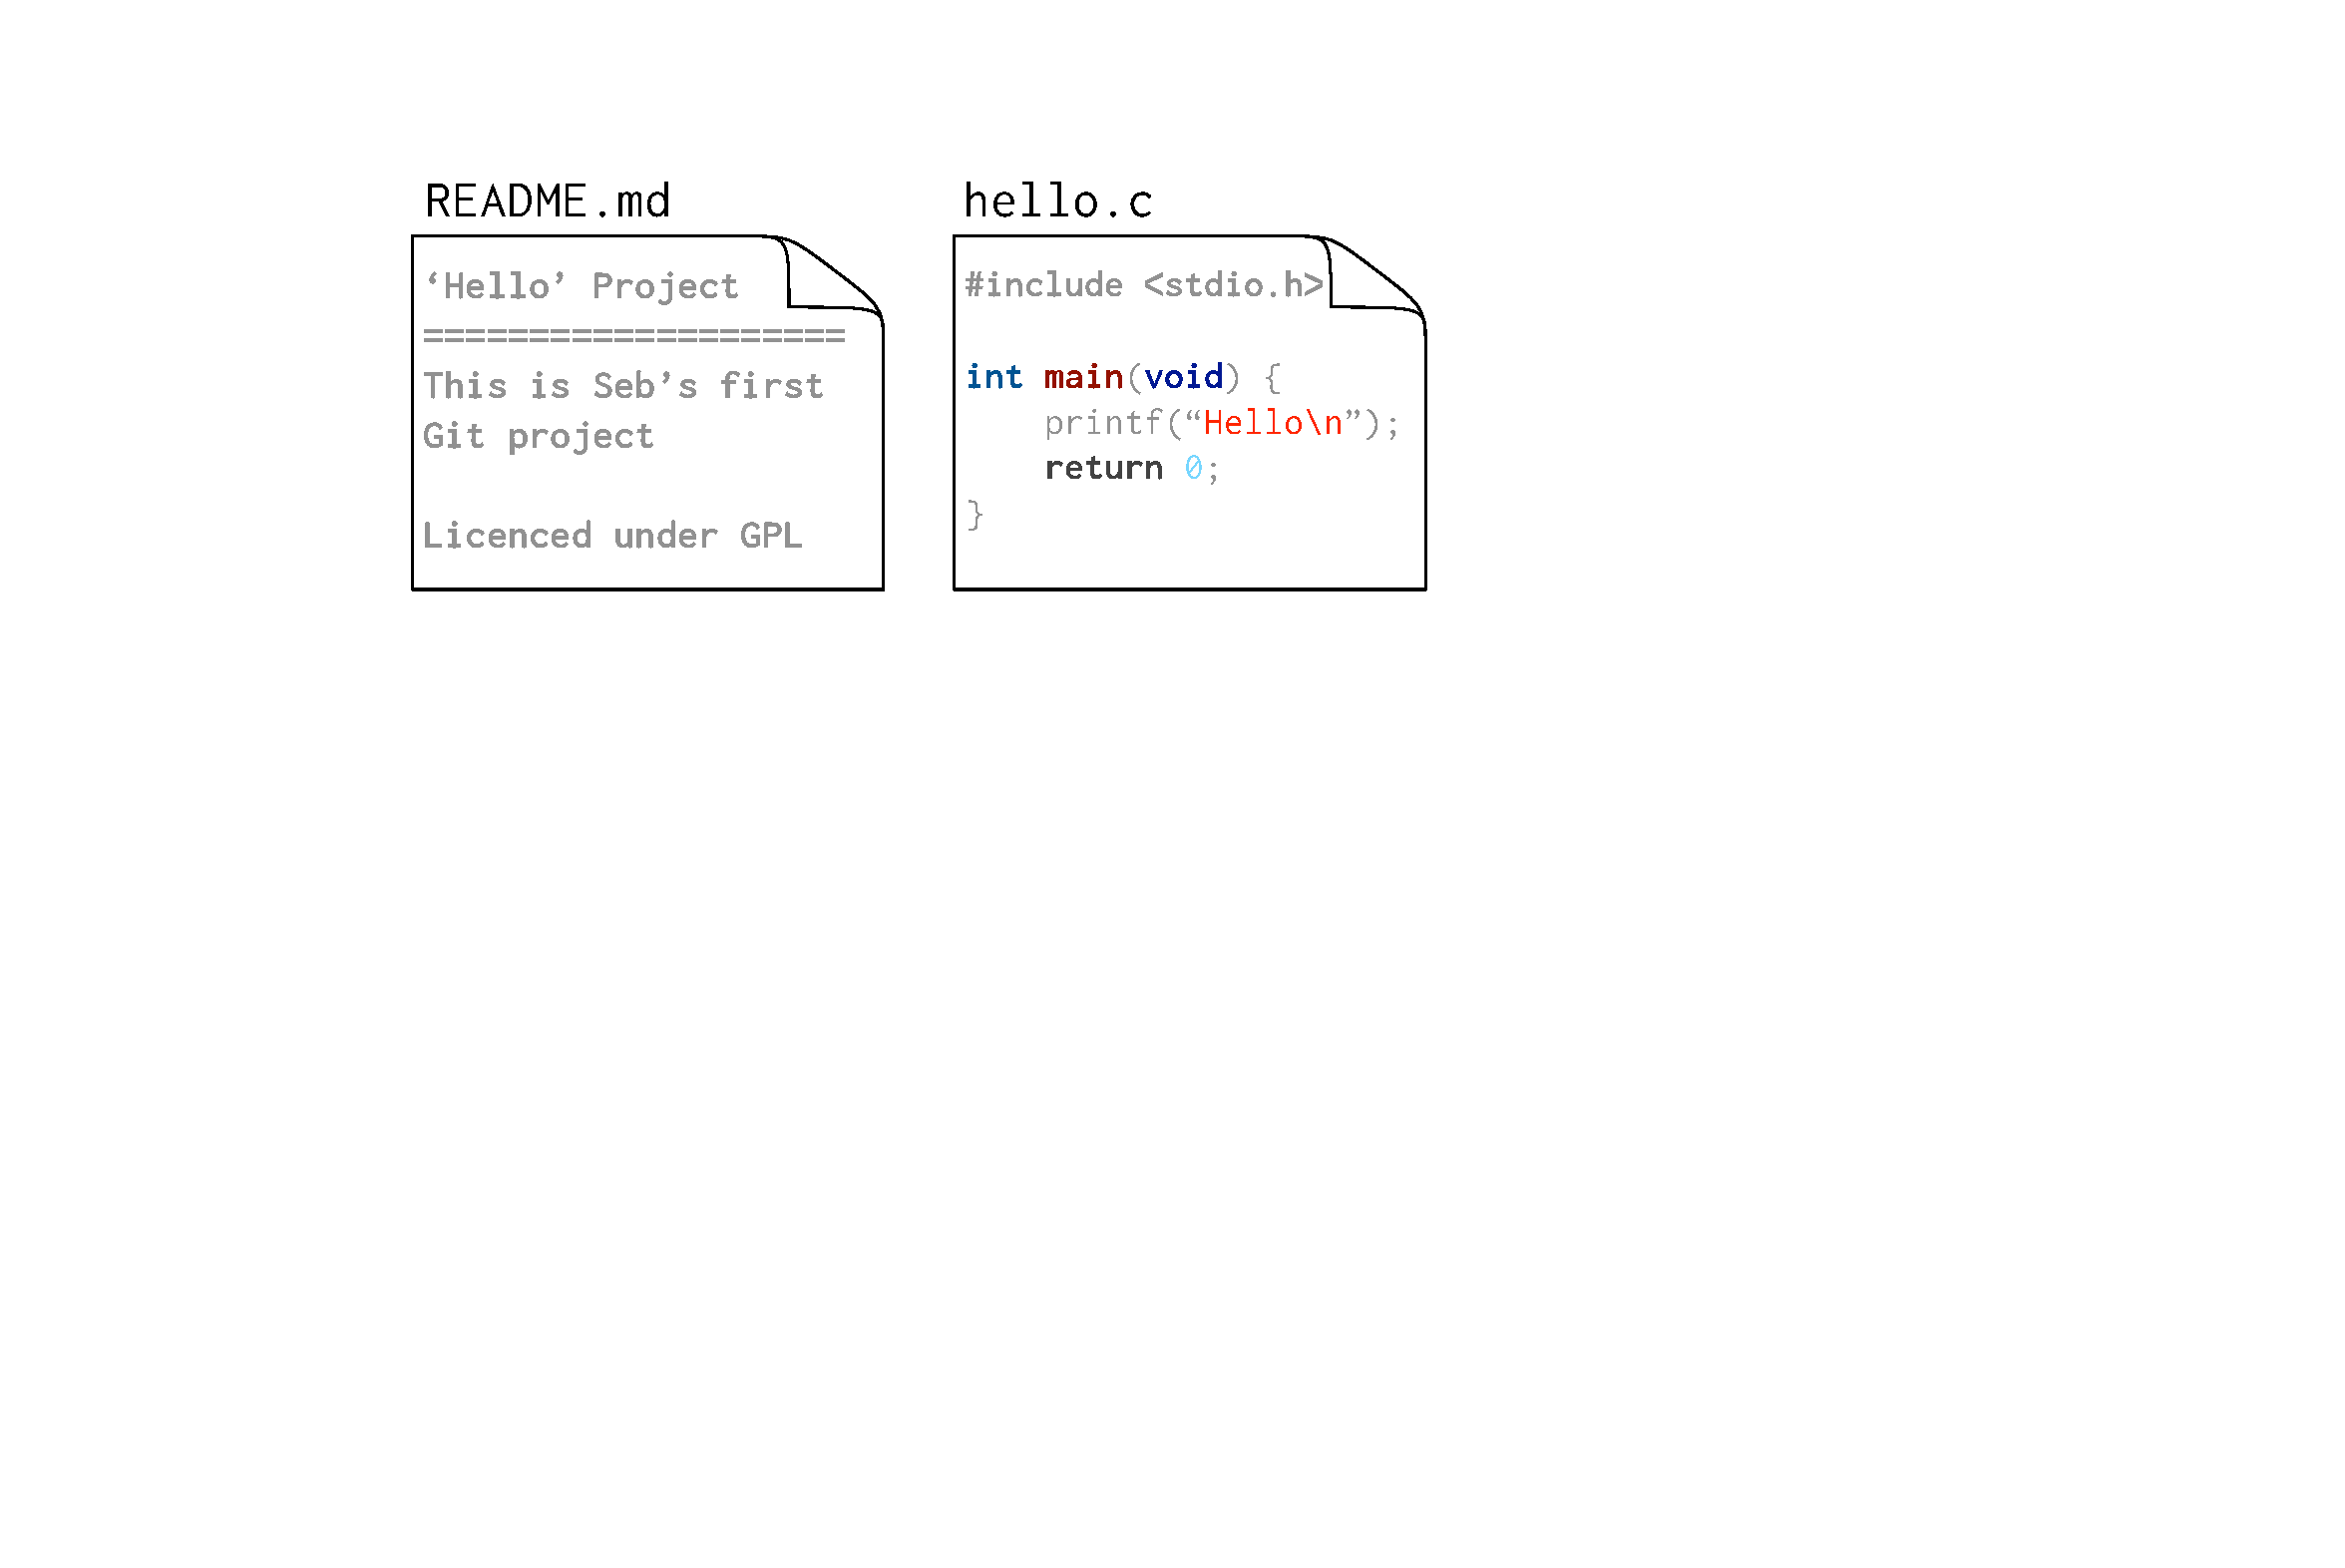
\includegraphics [height=0.95\textheight]{delta_vs_snapshot_example-001.pdf}}
  \only<2>{\includegraphics [height=0.95\textheight]{delta_vs_snapshot_example-002.pdf}}
  \only<3>{\includegraphics [height=0.95\textheight]{delta_vs_snapshot_example-003.pdf}}
  \only<4>{\includegraphics [height=0.95\textheight]{delta_vs_snapshot_example-004.pdf}}
  \only<5>{\includegraphics [height=0.95\textheight]{delta_vs_snapshot_example-005.pdf}}
  \only<6>{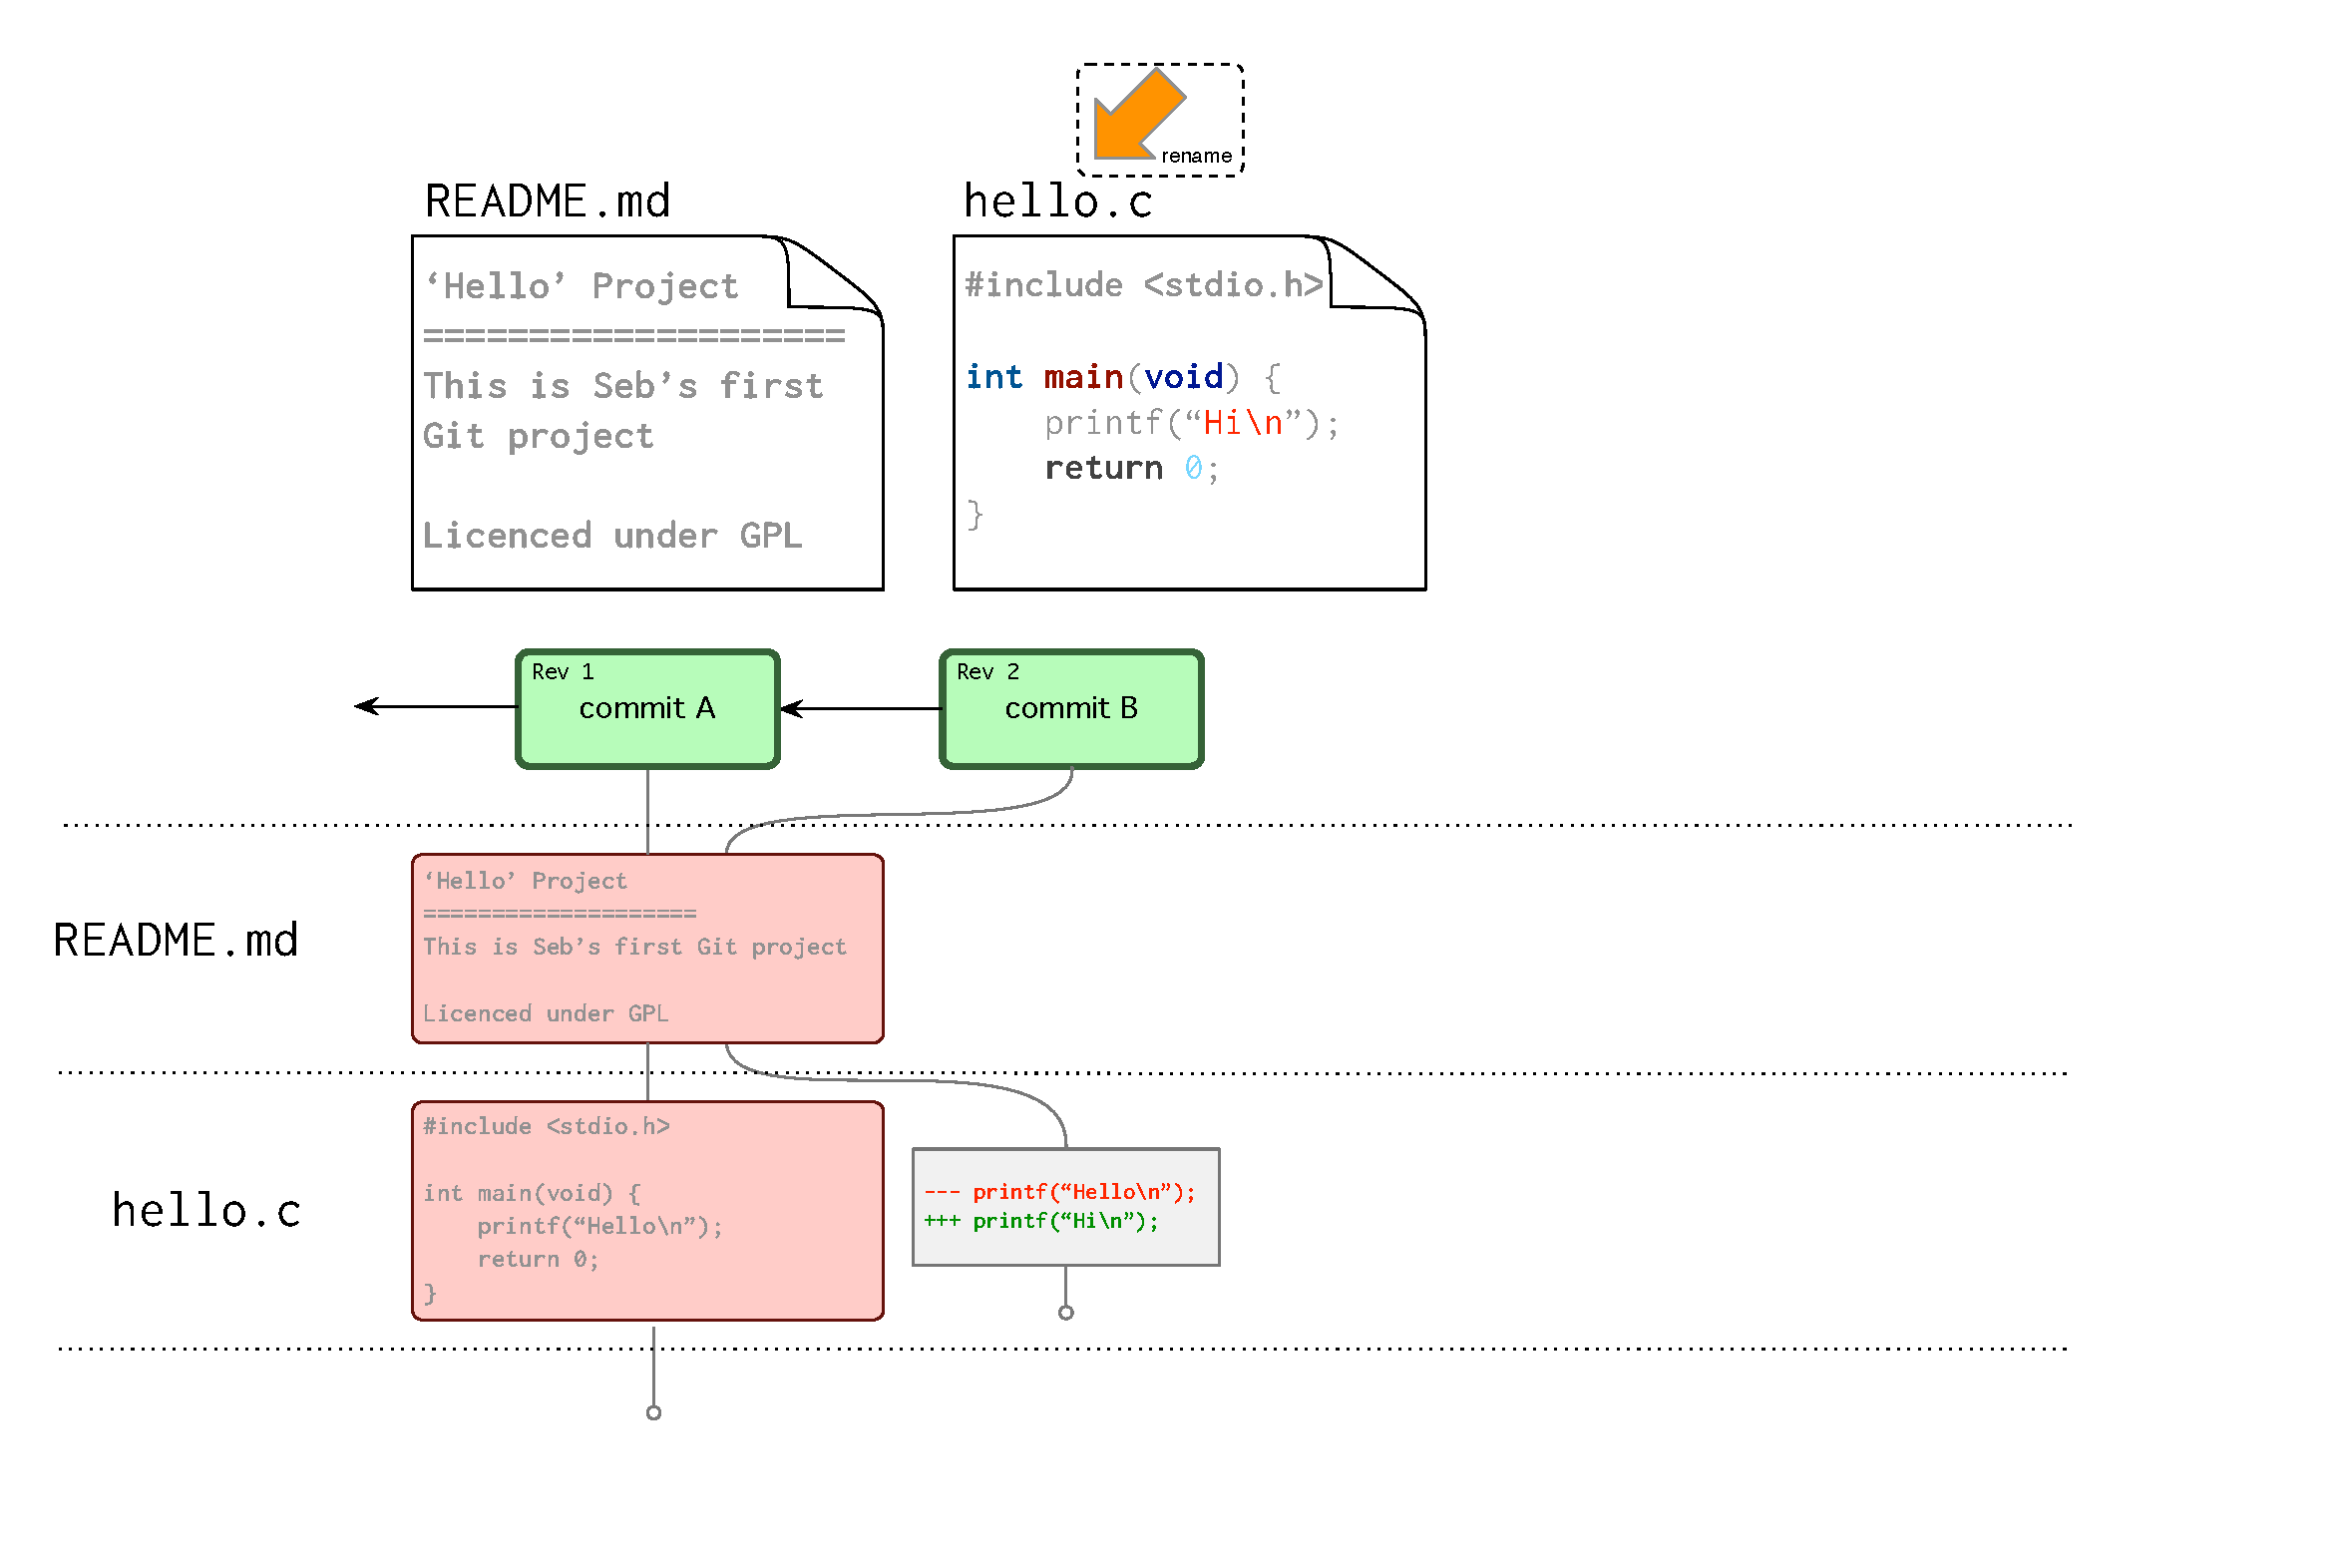
\includegraphics [height=0.95\textheight]{delta_vs_snapshot_example-006.pdf}}
  \only<7>{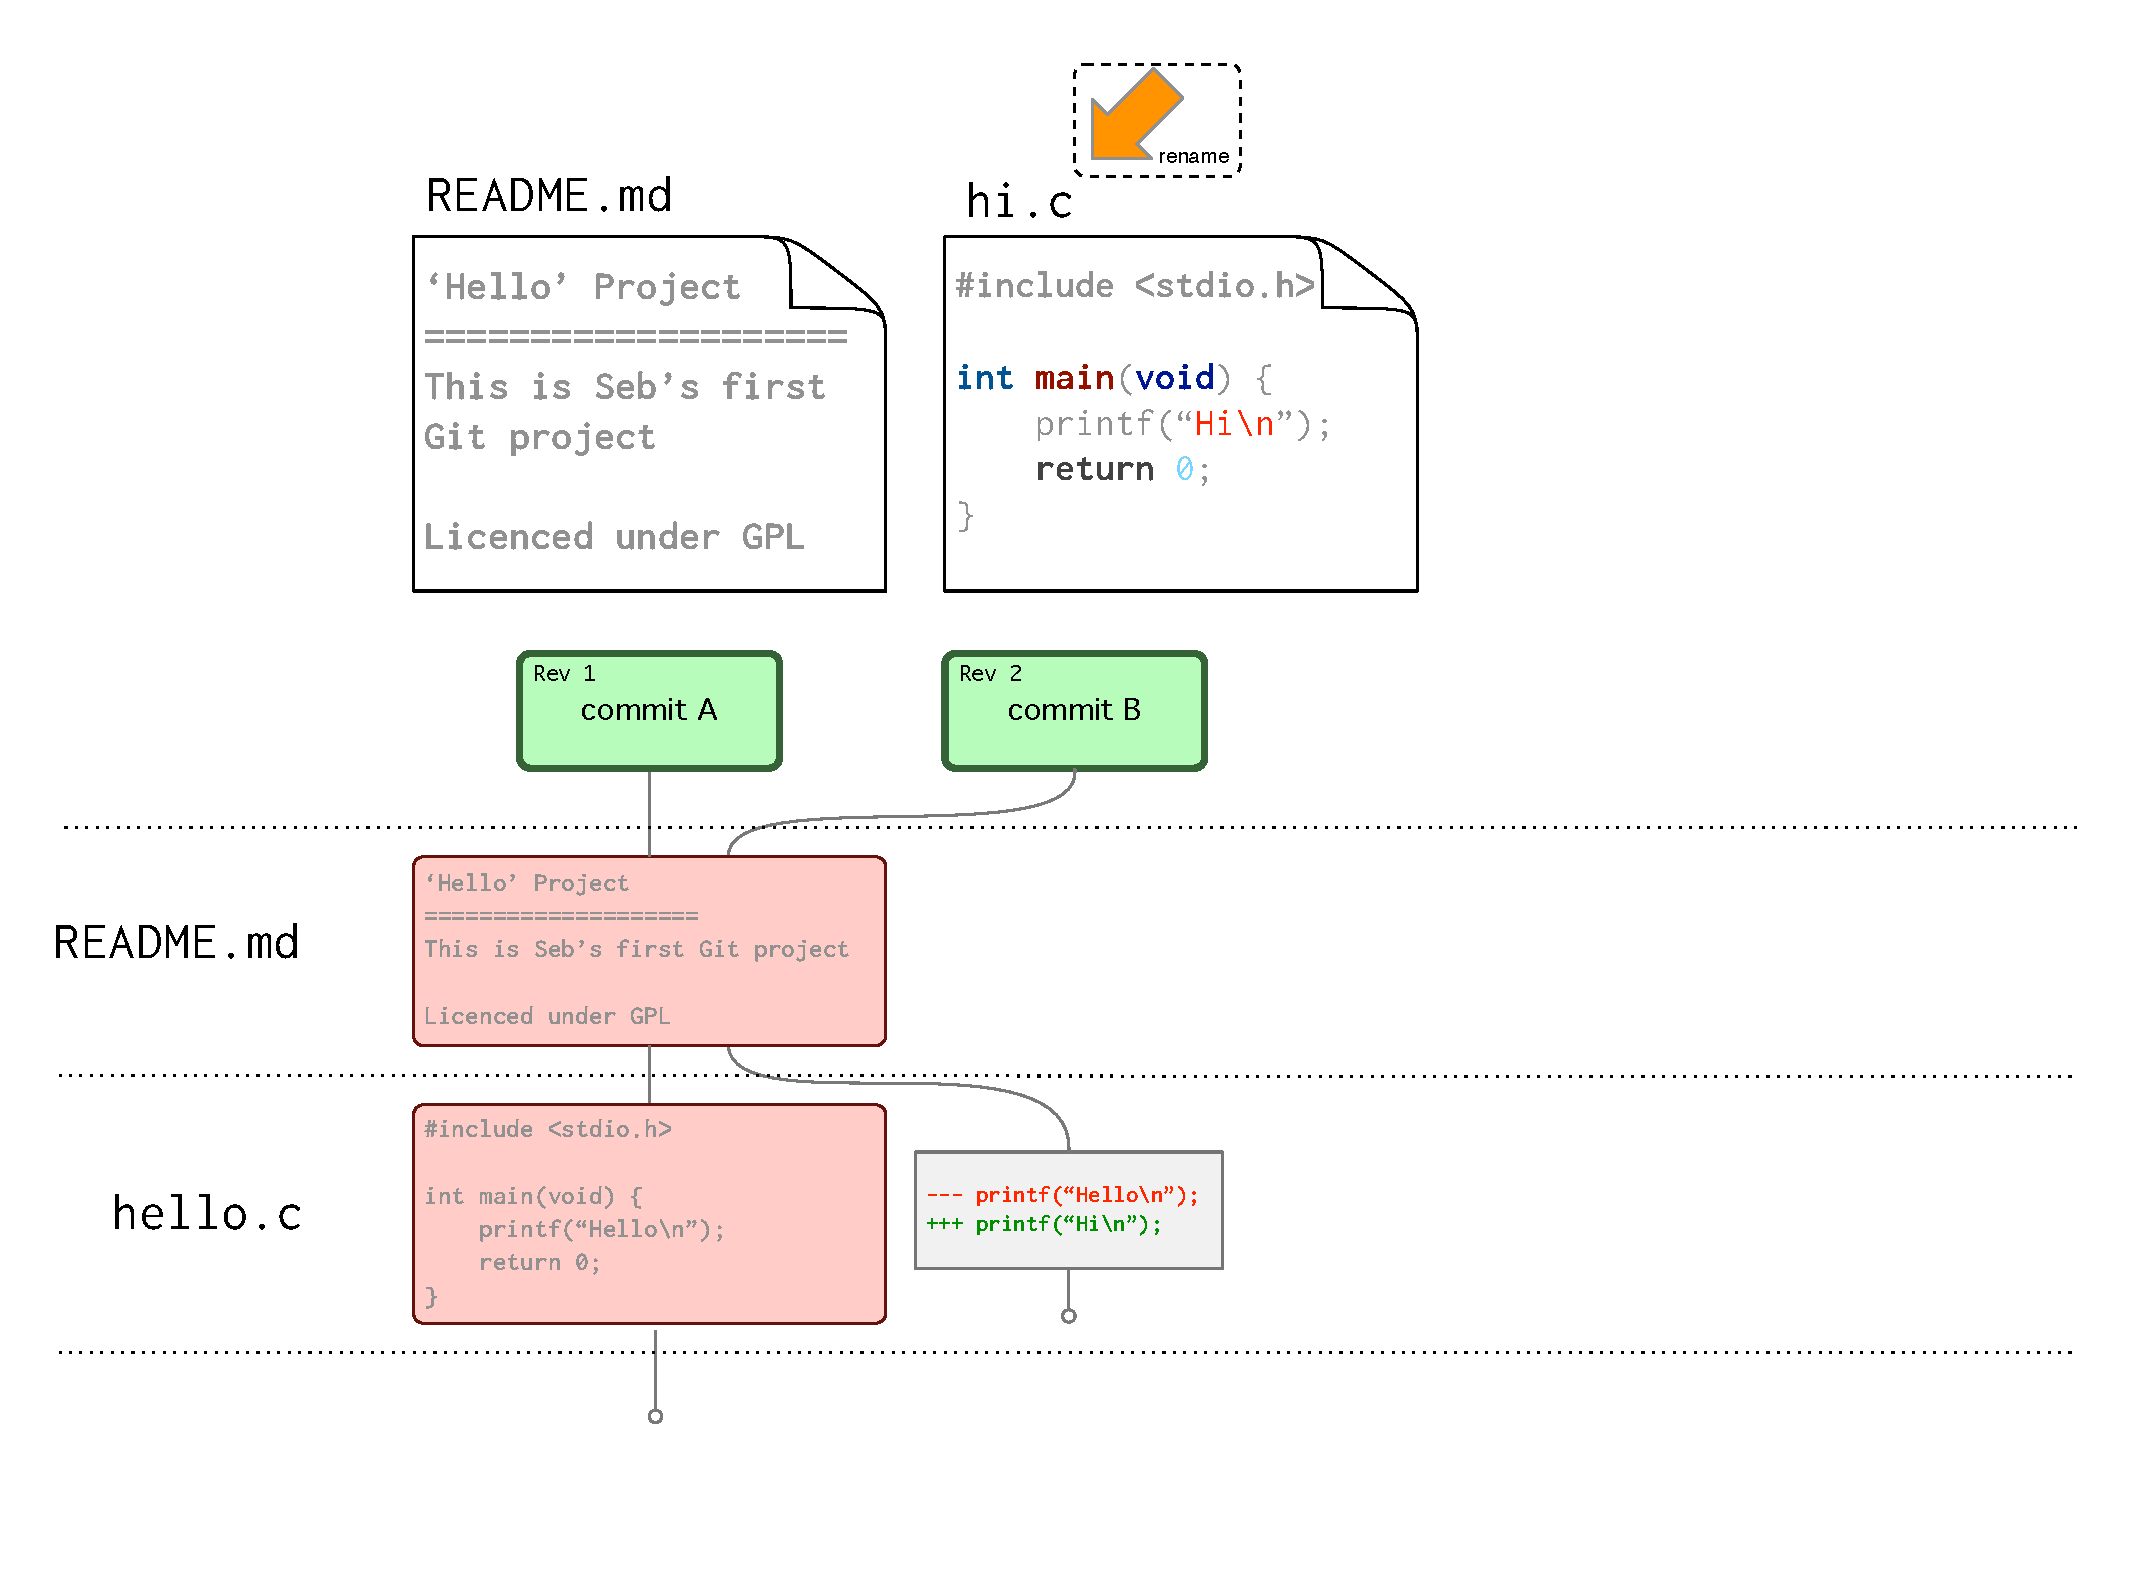
\includegraphics [height=0.95\textheight]{delta_vs_snapshot_example-007.pdf}}
  \only<8>{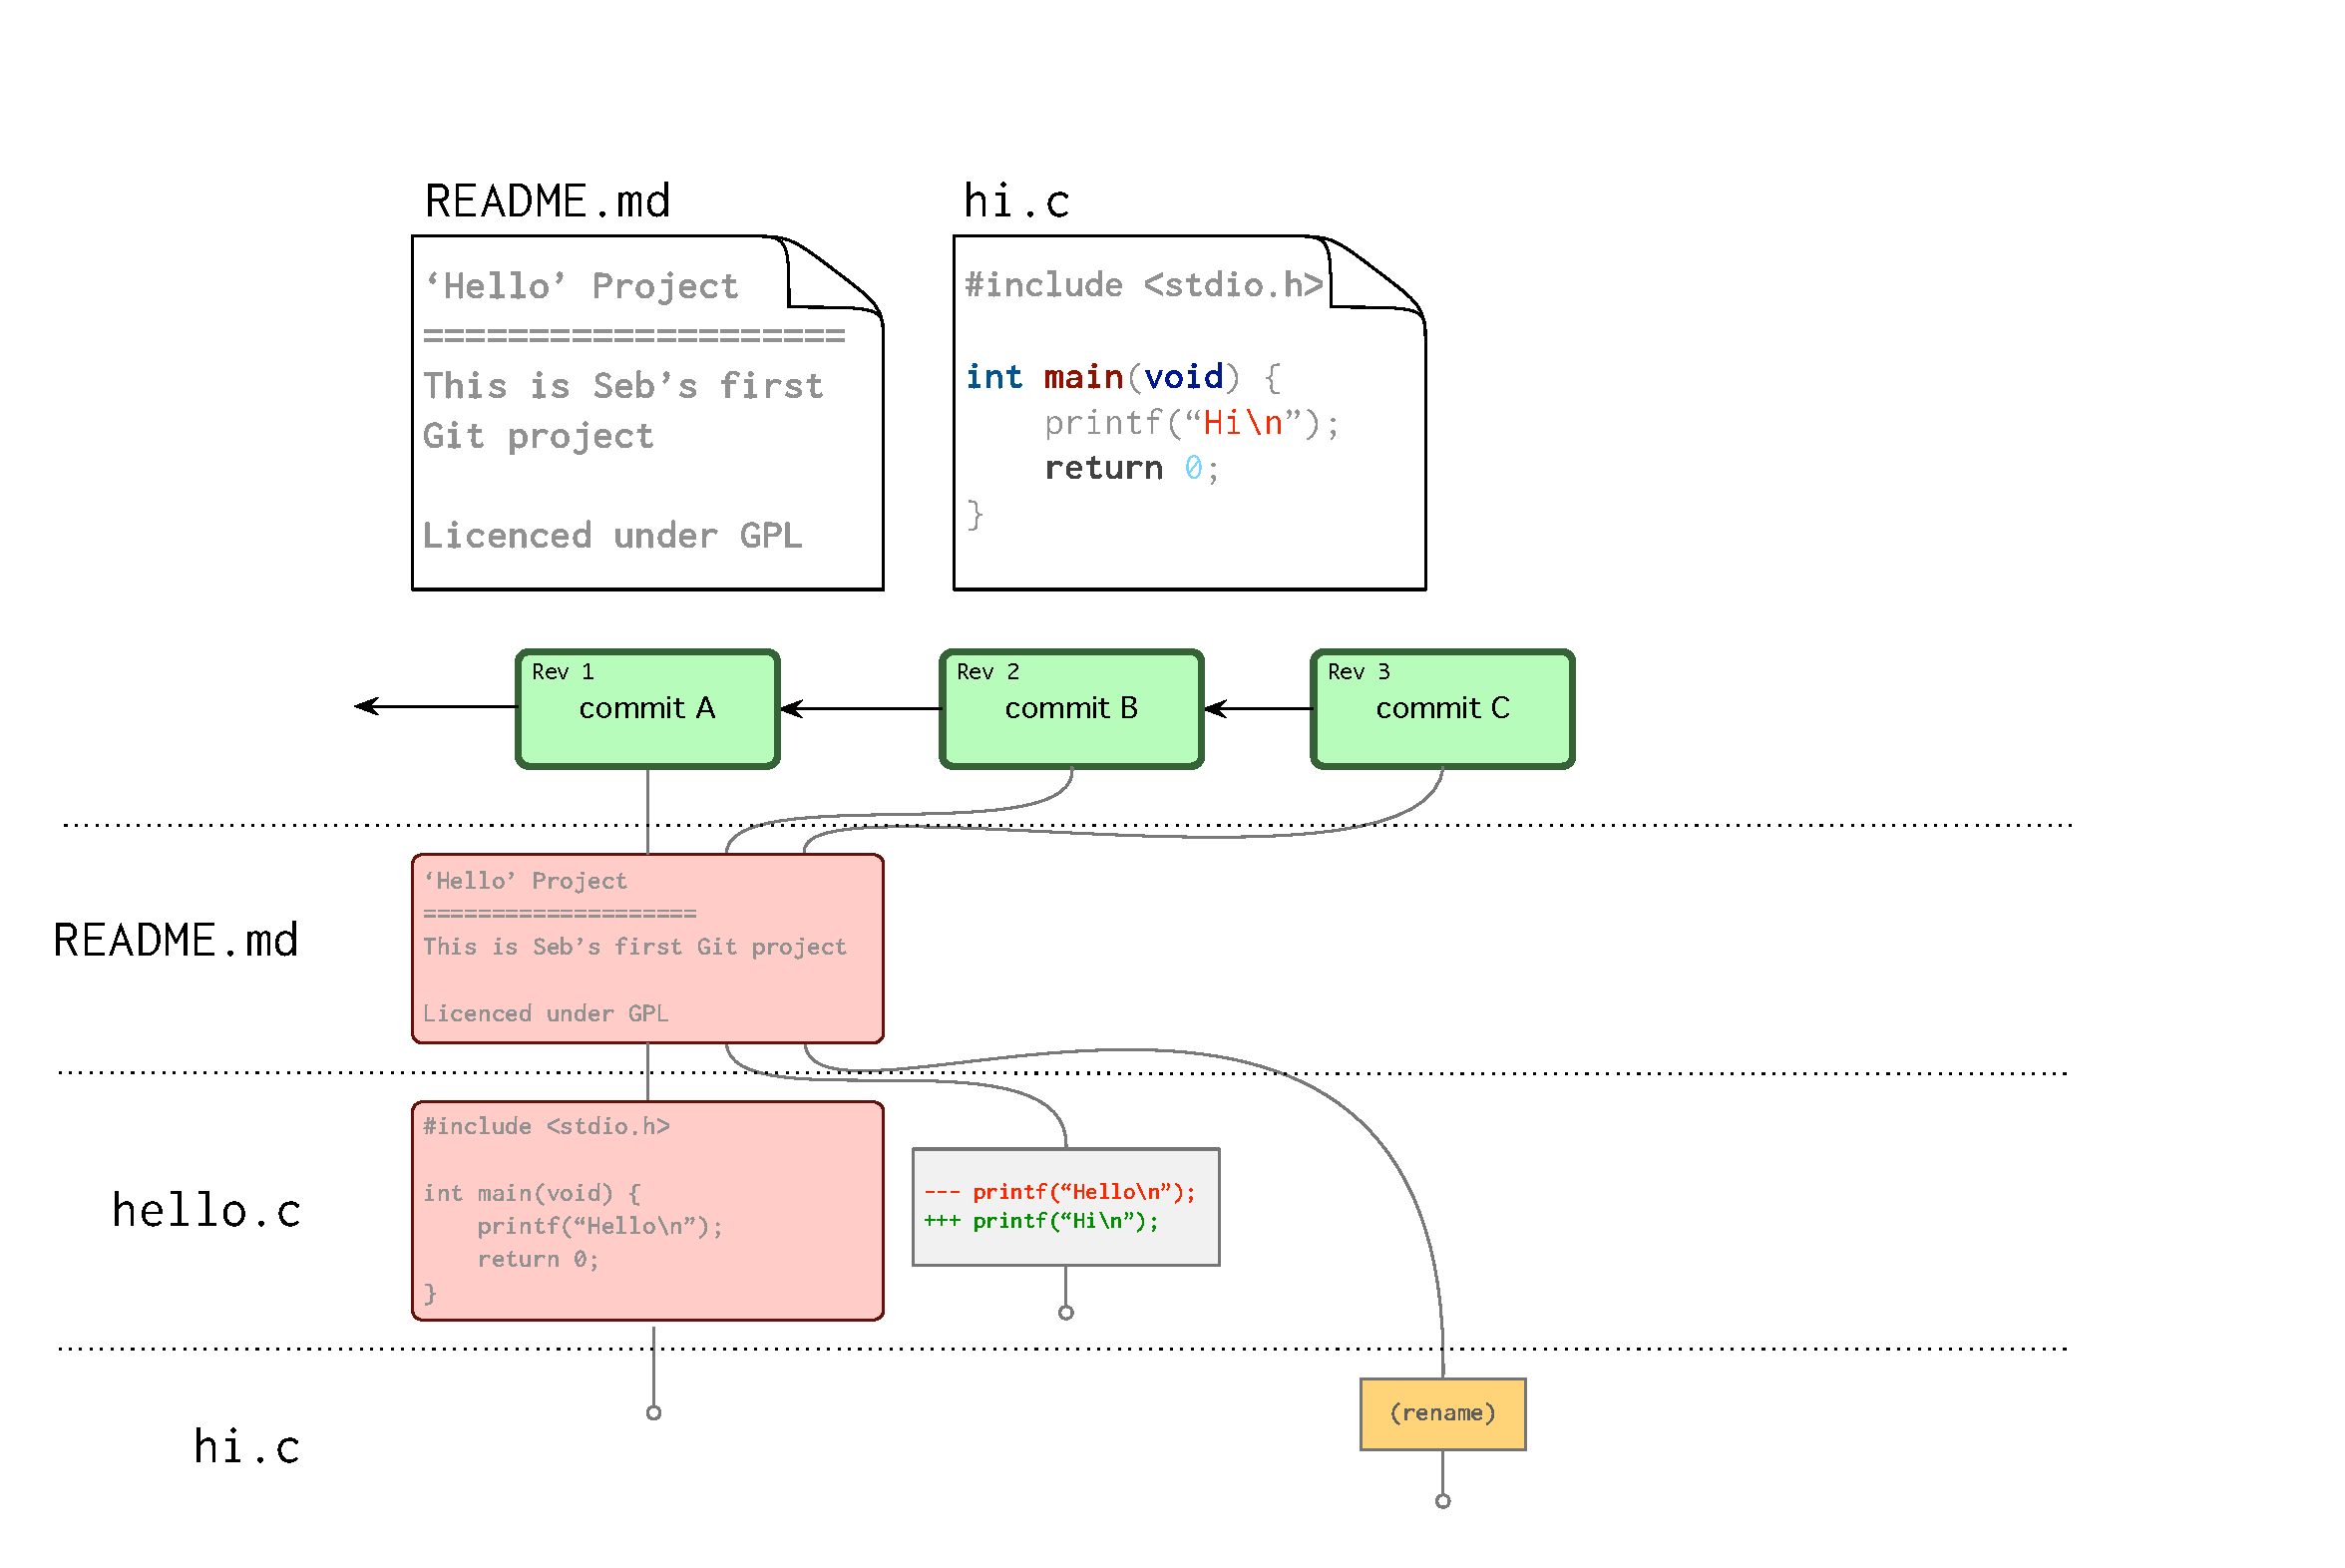
\includegraphics [height=0.95\textheight]{delta_vs_snapshot_example-008.pdf}}
  \only<9>{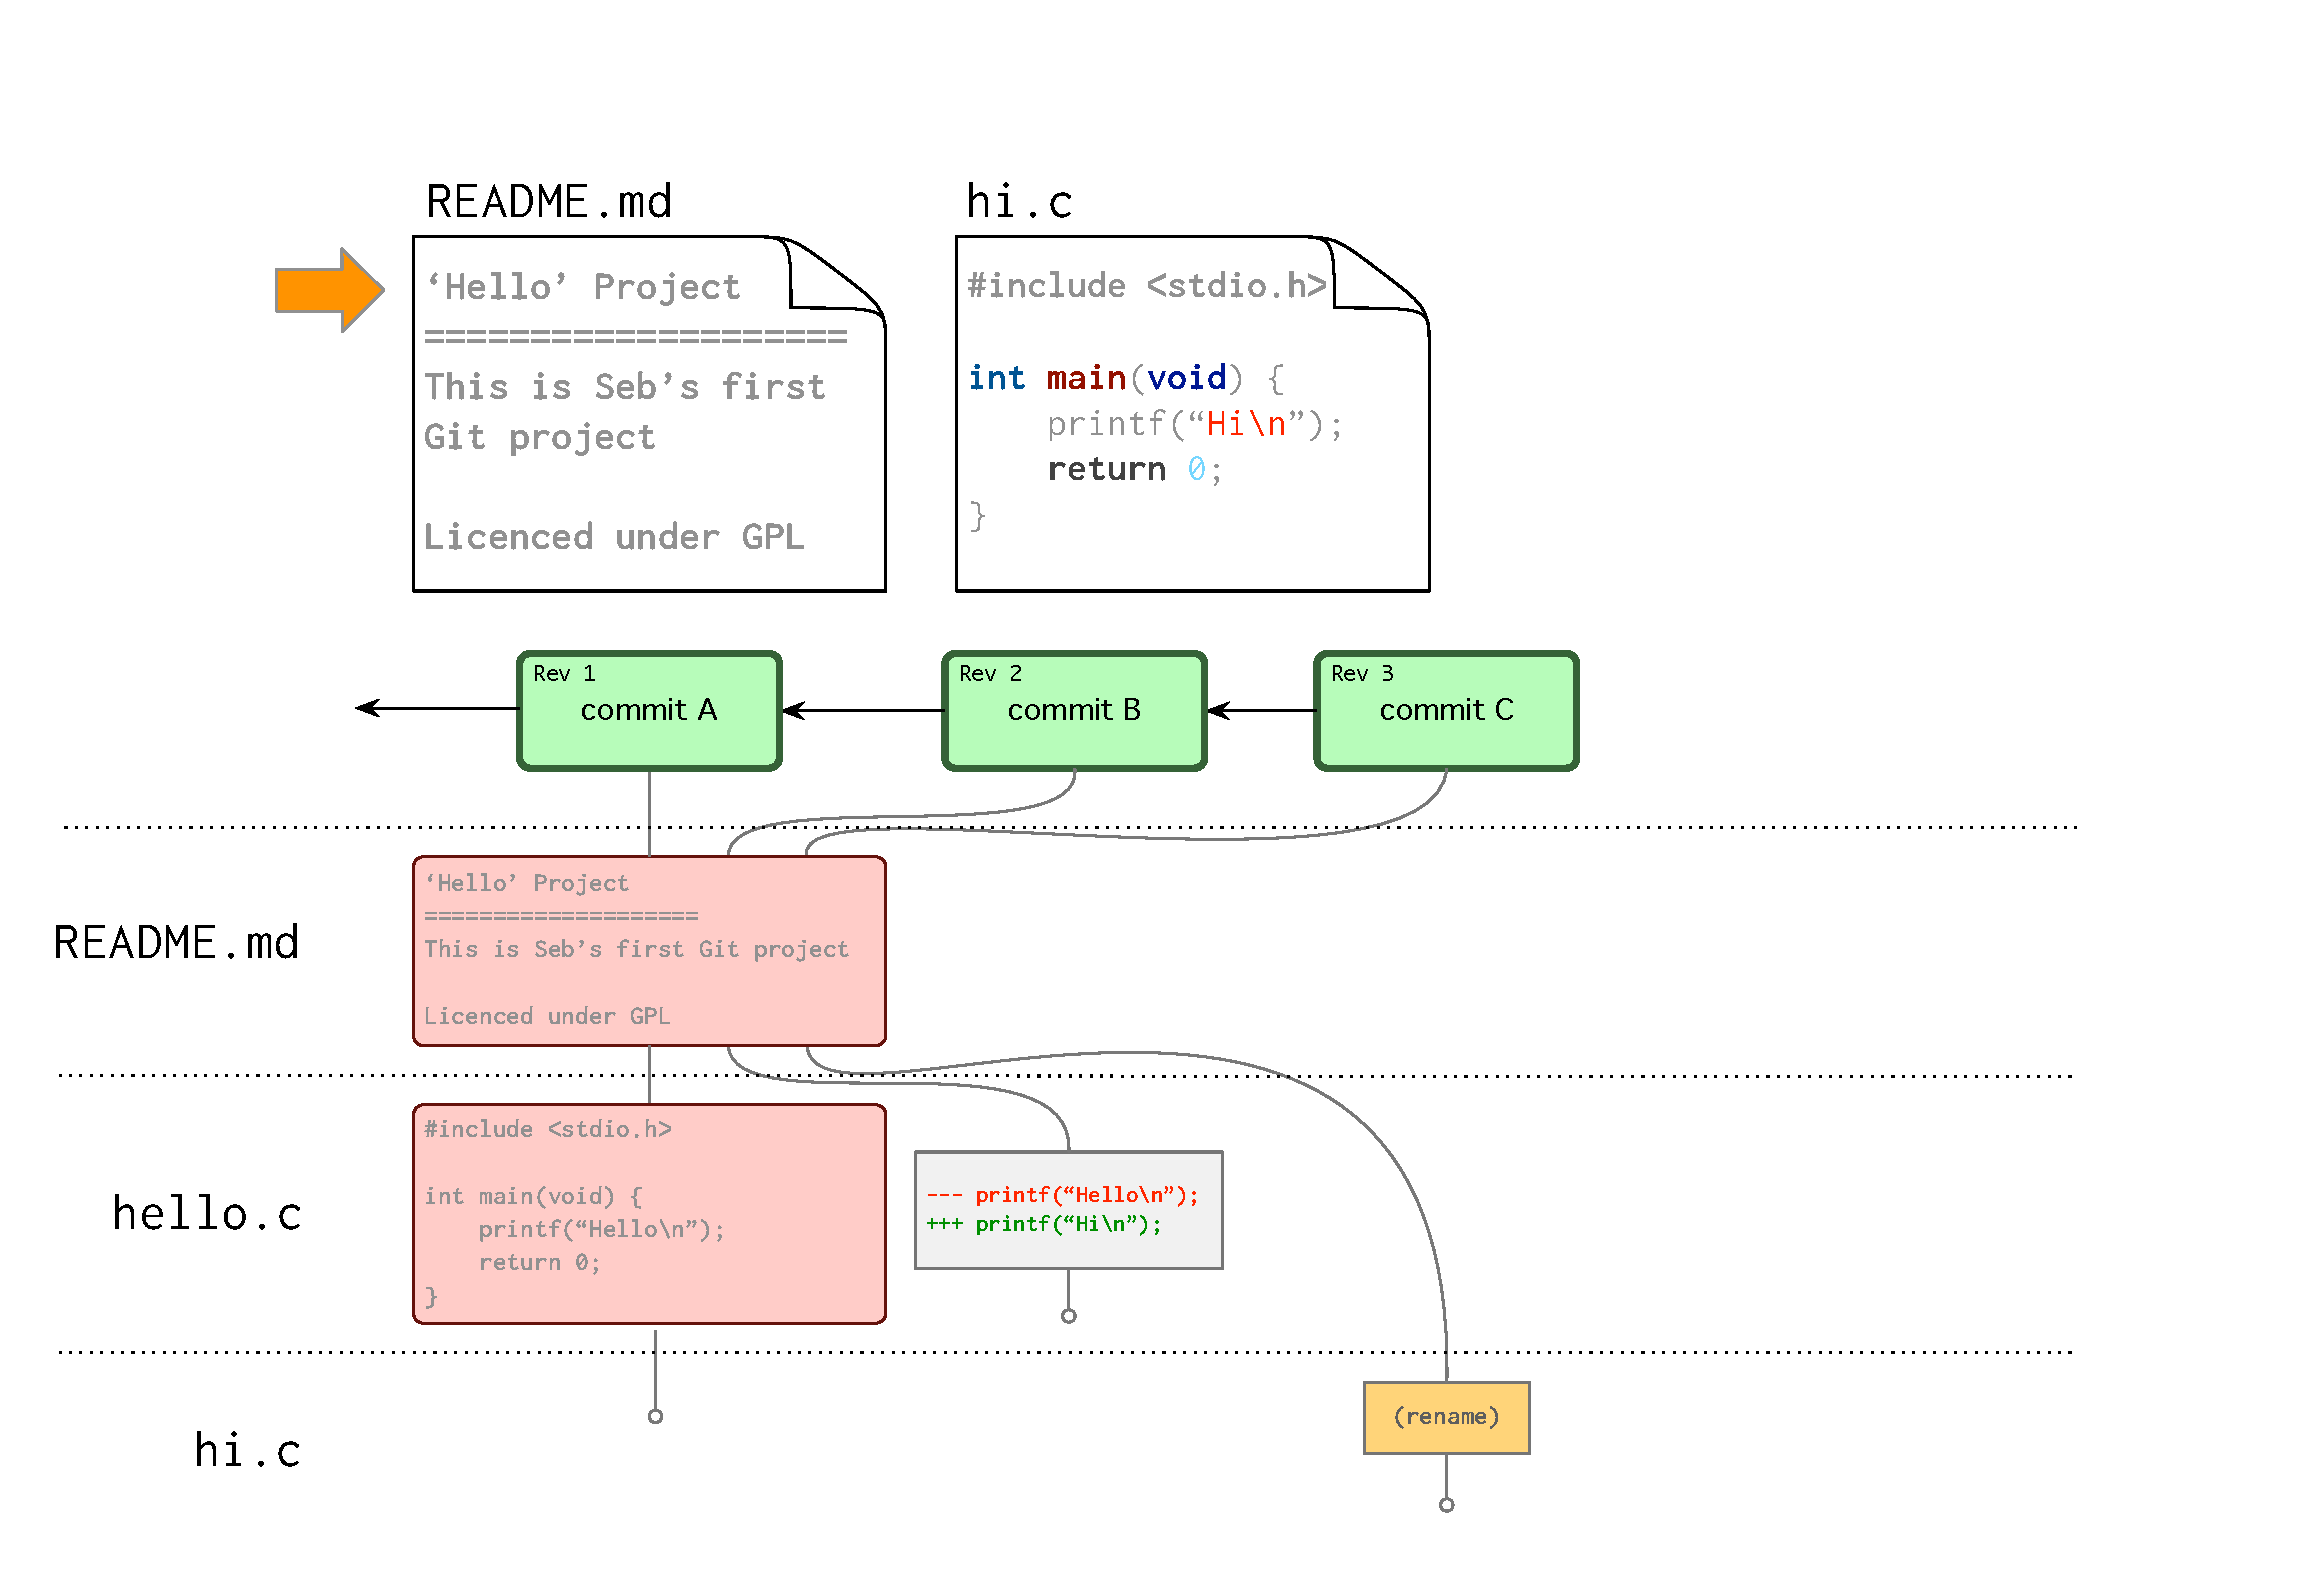
\includegraphics [height=0.95\textheight]{delta_vs_snapshot_example-009.pdf}}
  \only<10>{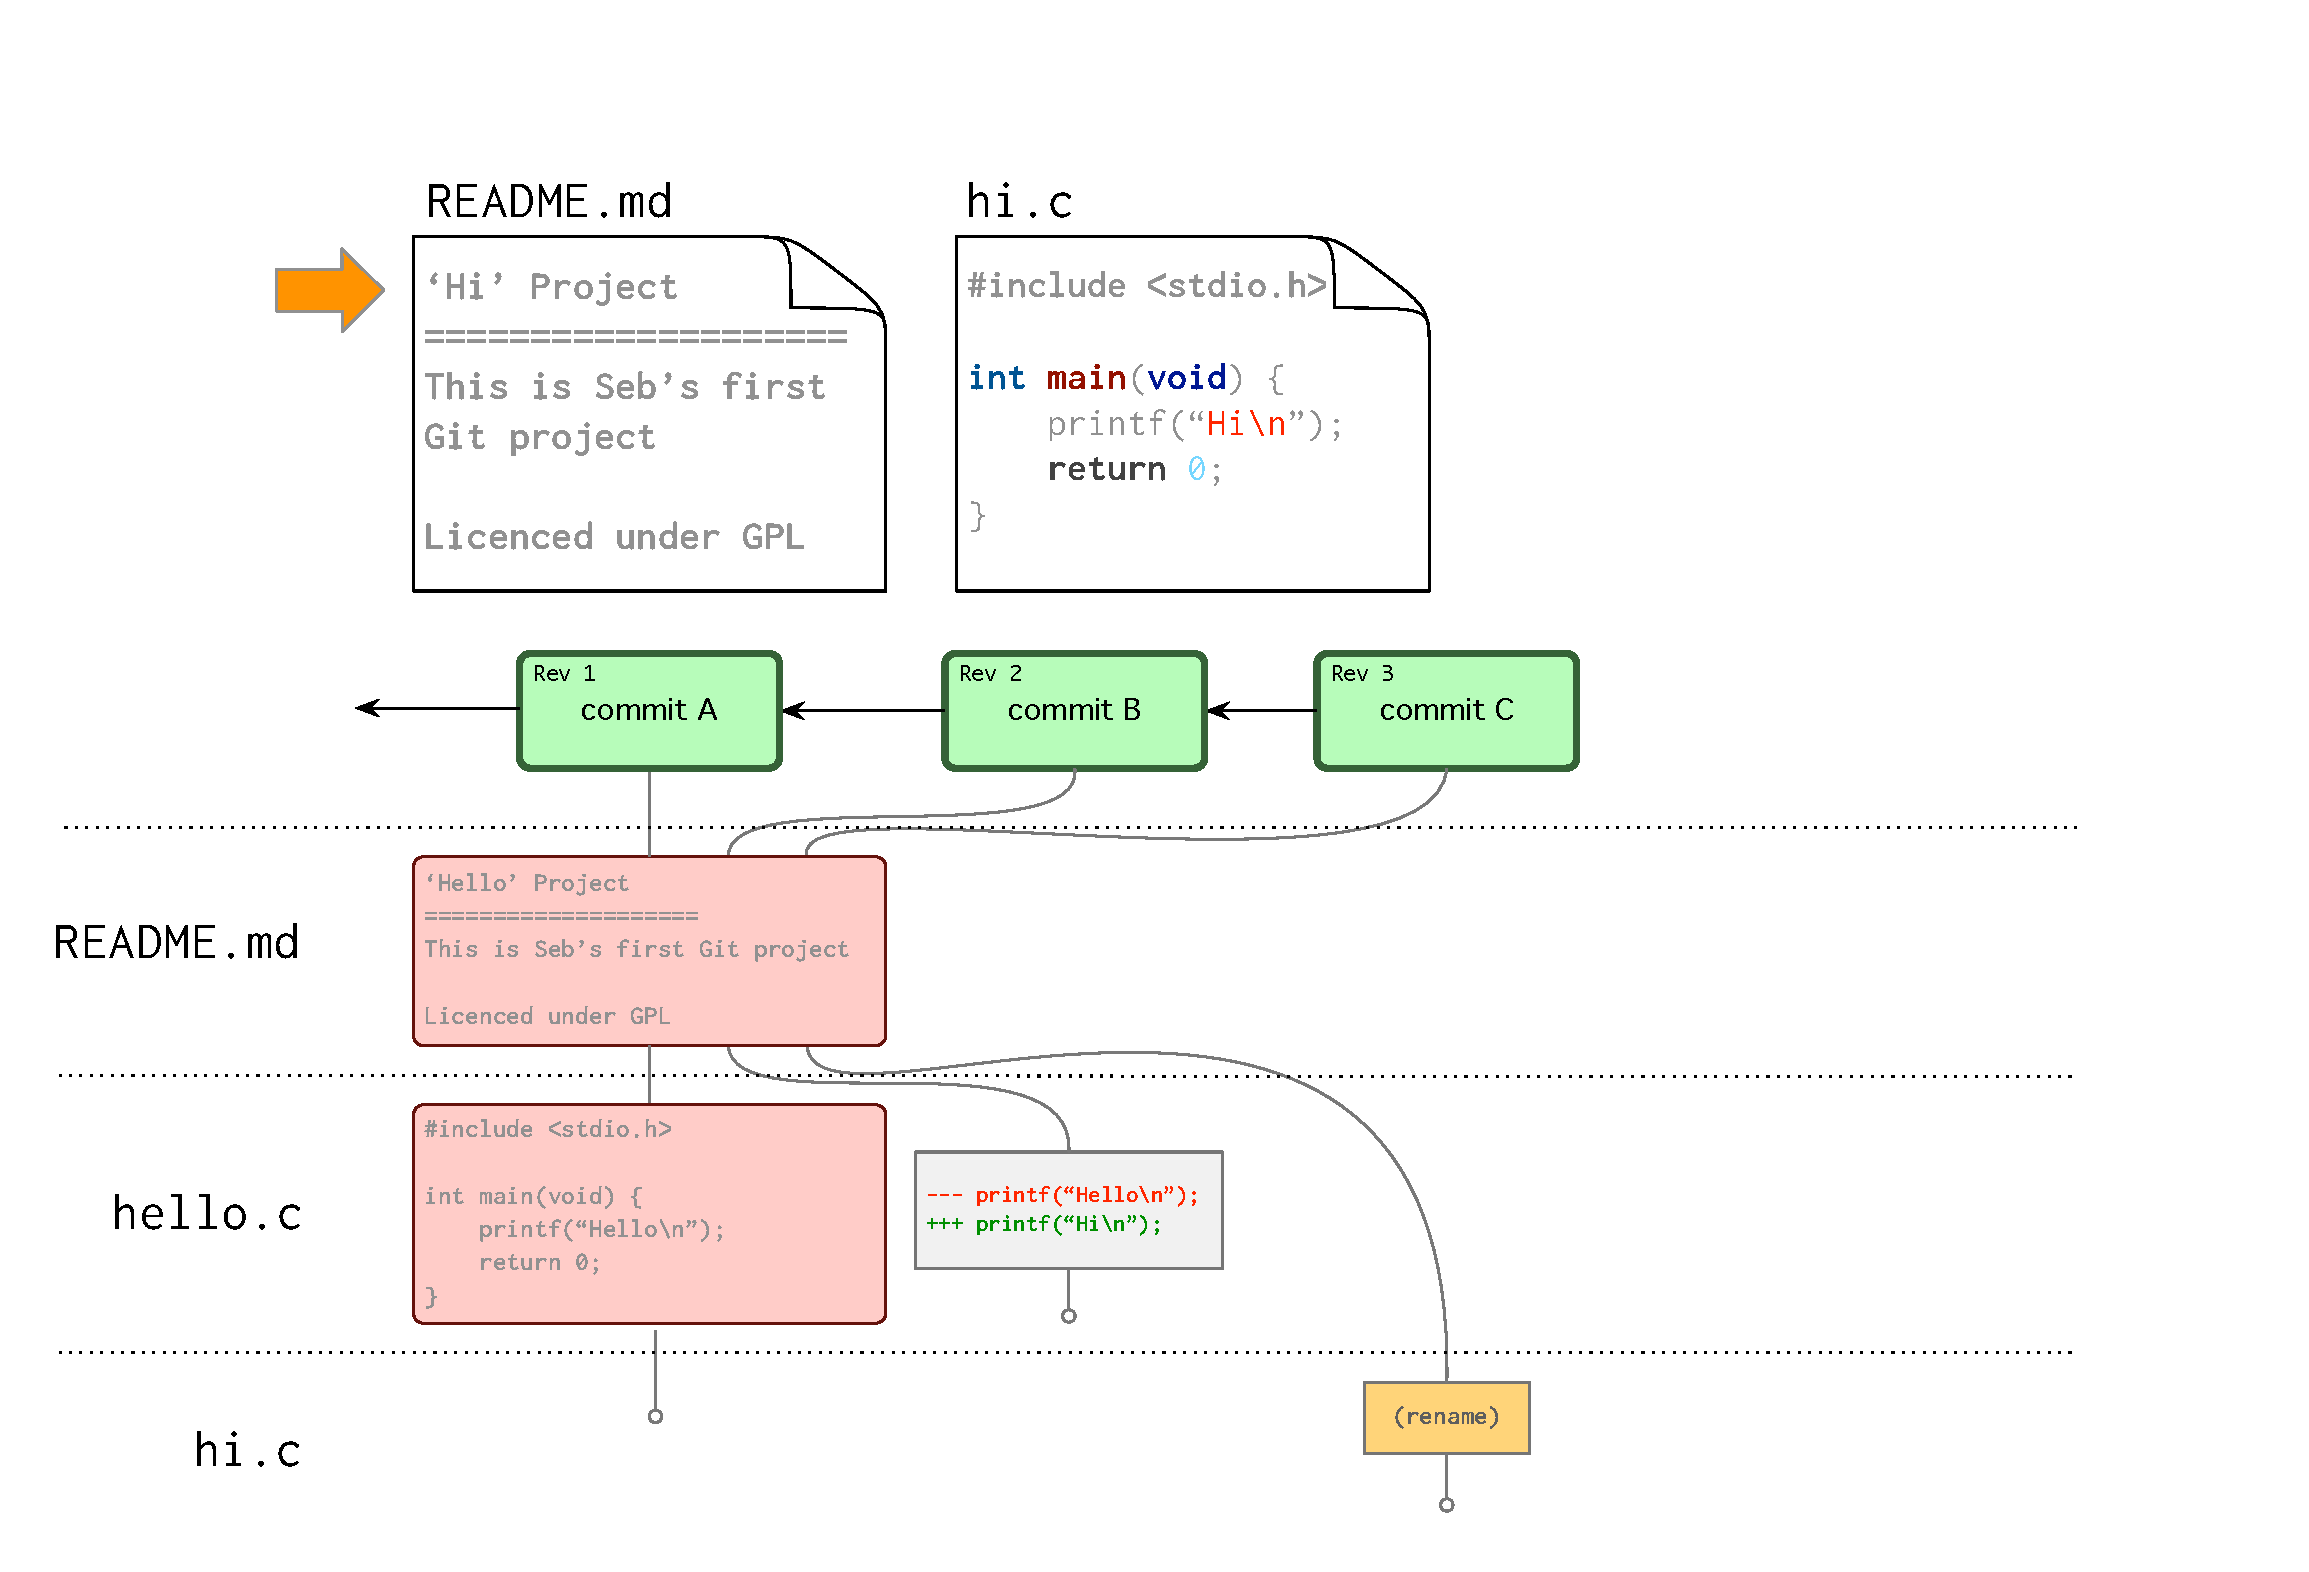
\includegraphics[height=0.95\textheight]{delta_vs_snapshot_example-010.pdf}}
  \only<11>{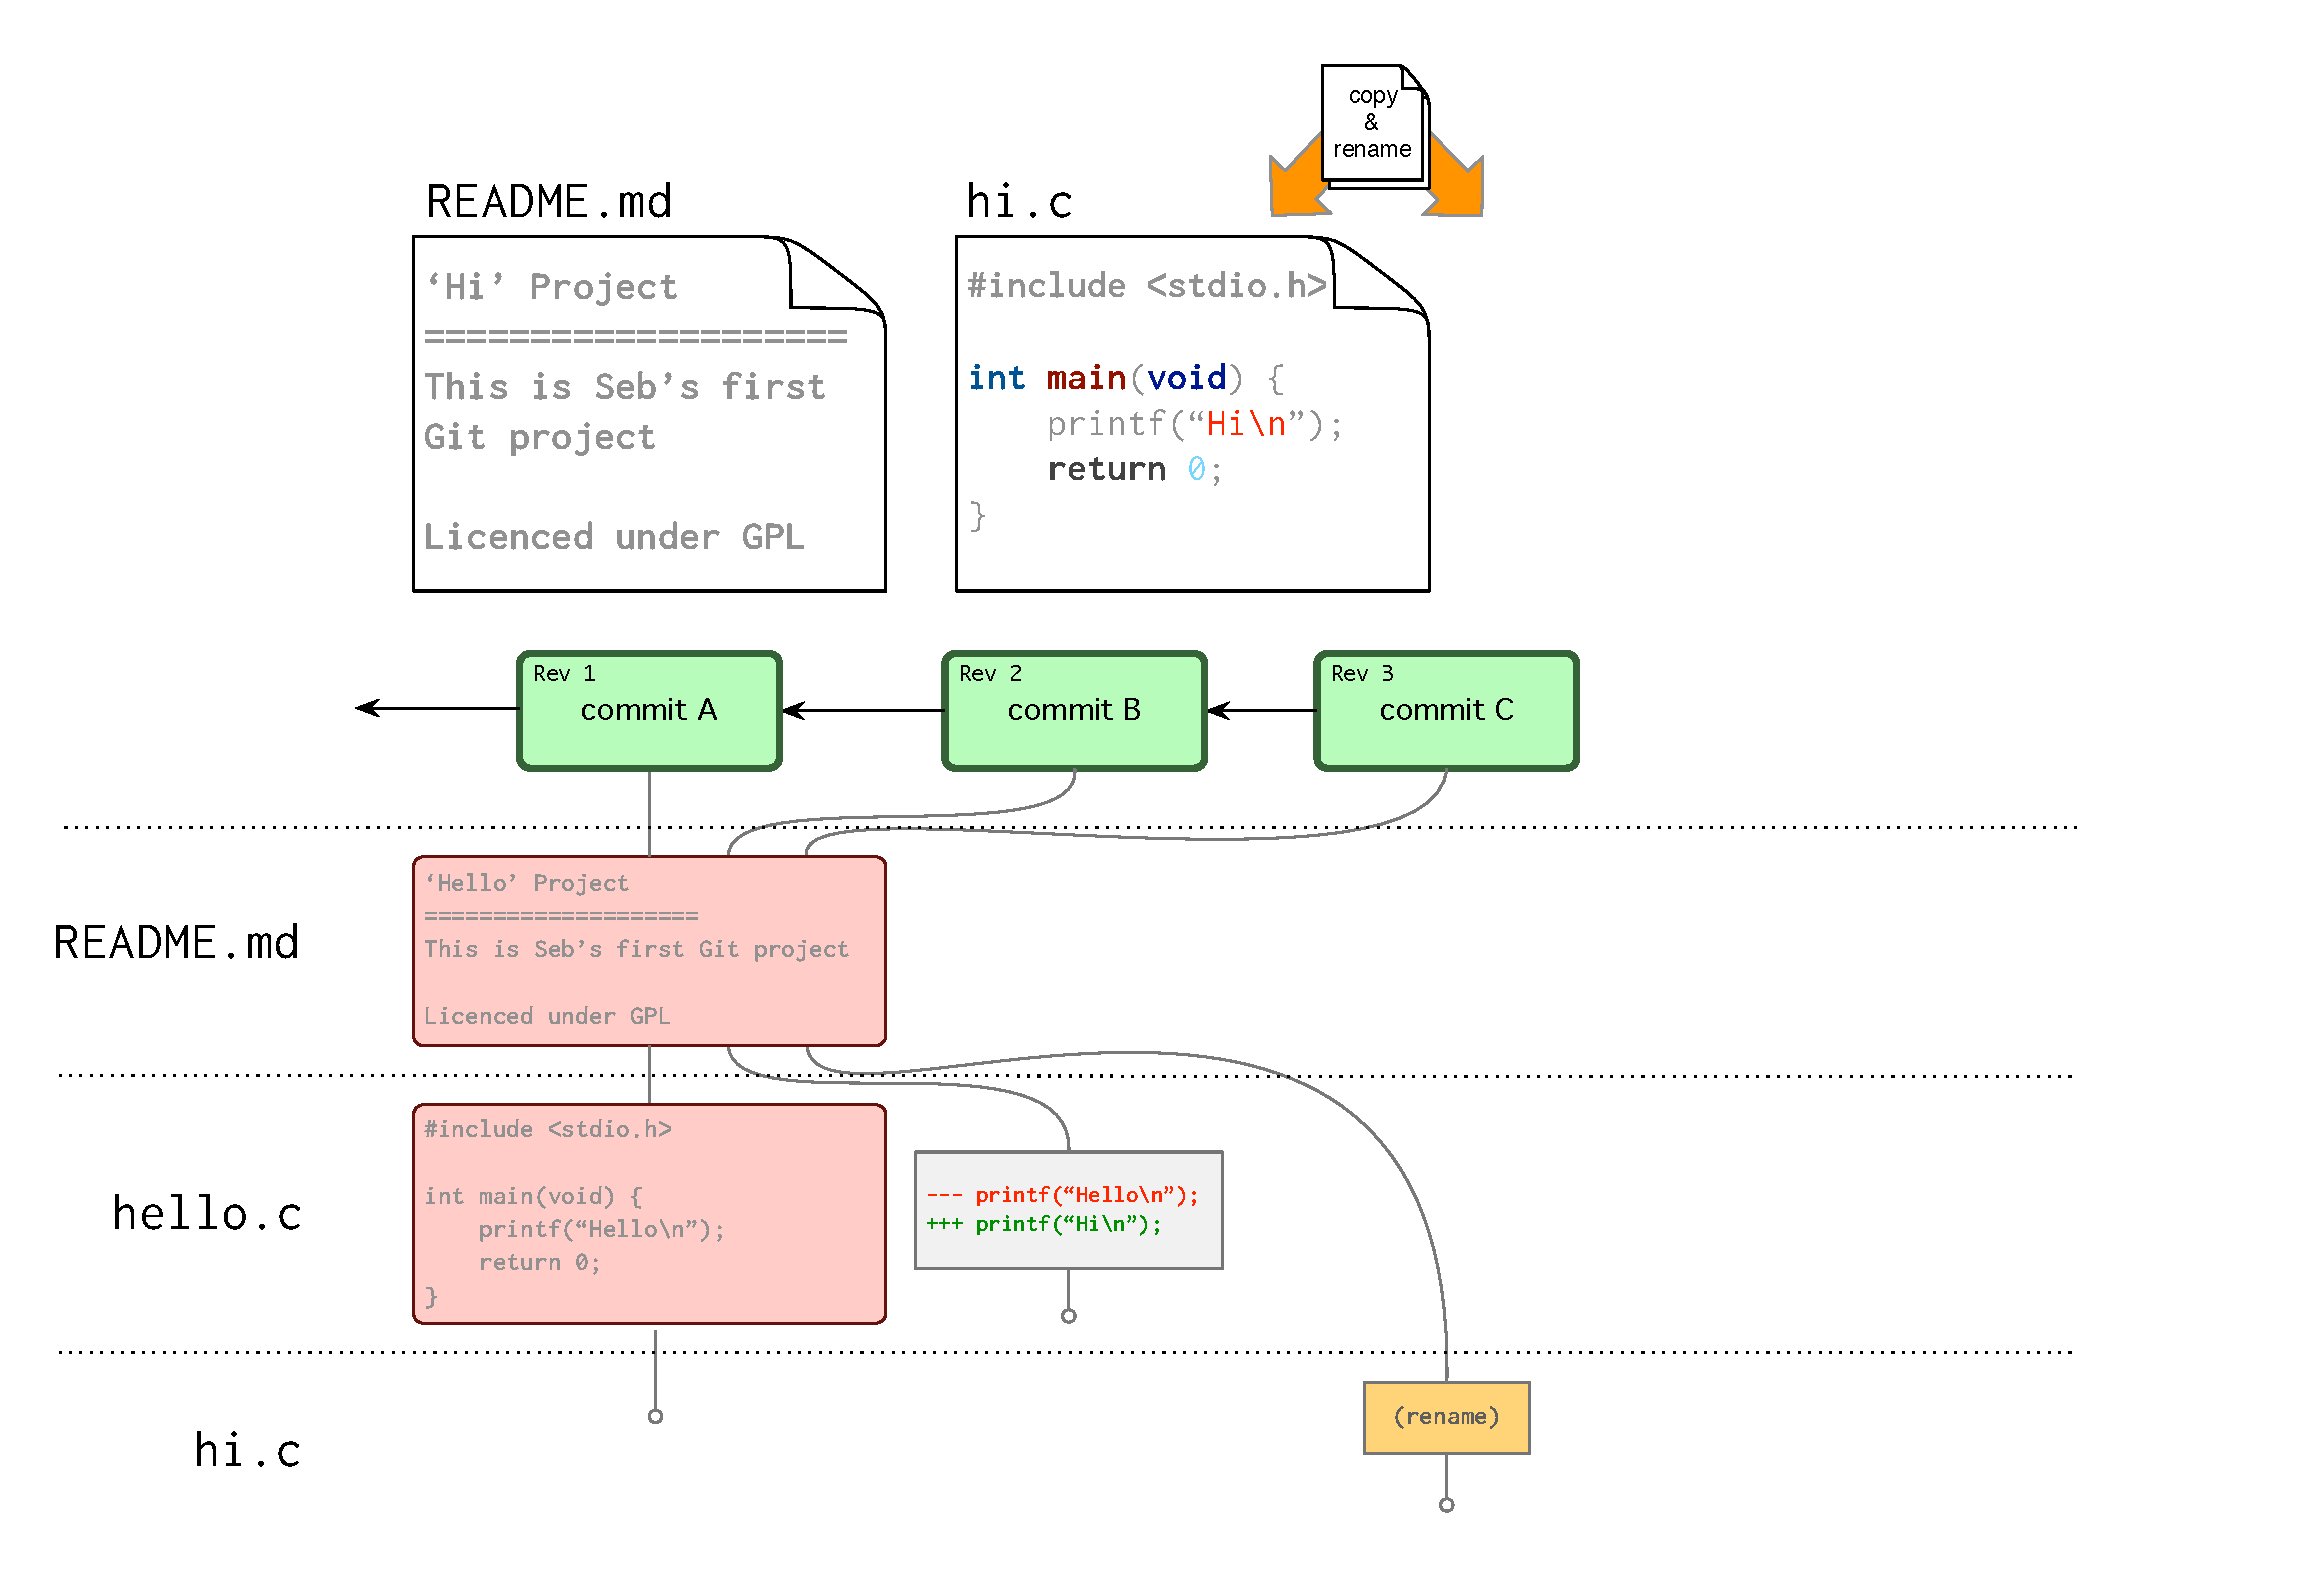
\includegraphics[height=0.95\textheight]{delta_vs_snapshot_example-011.pdf}}
  \only<12>{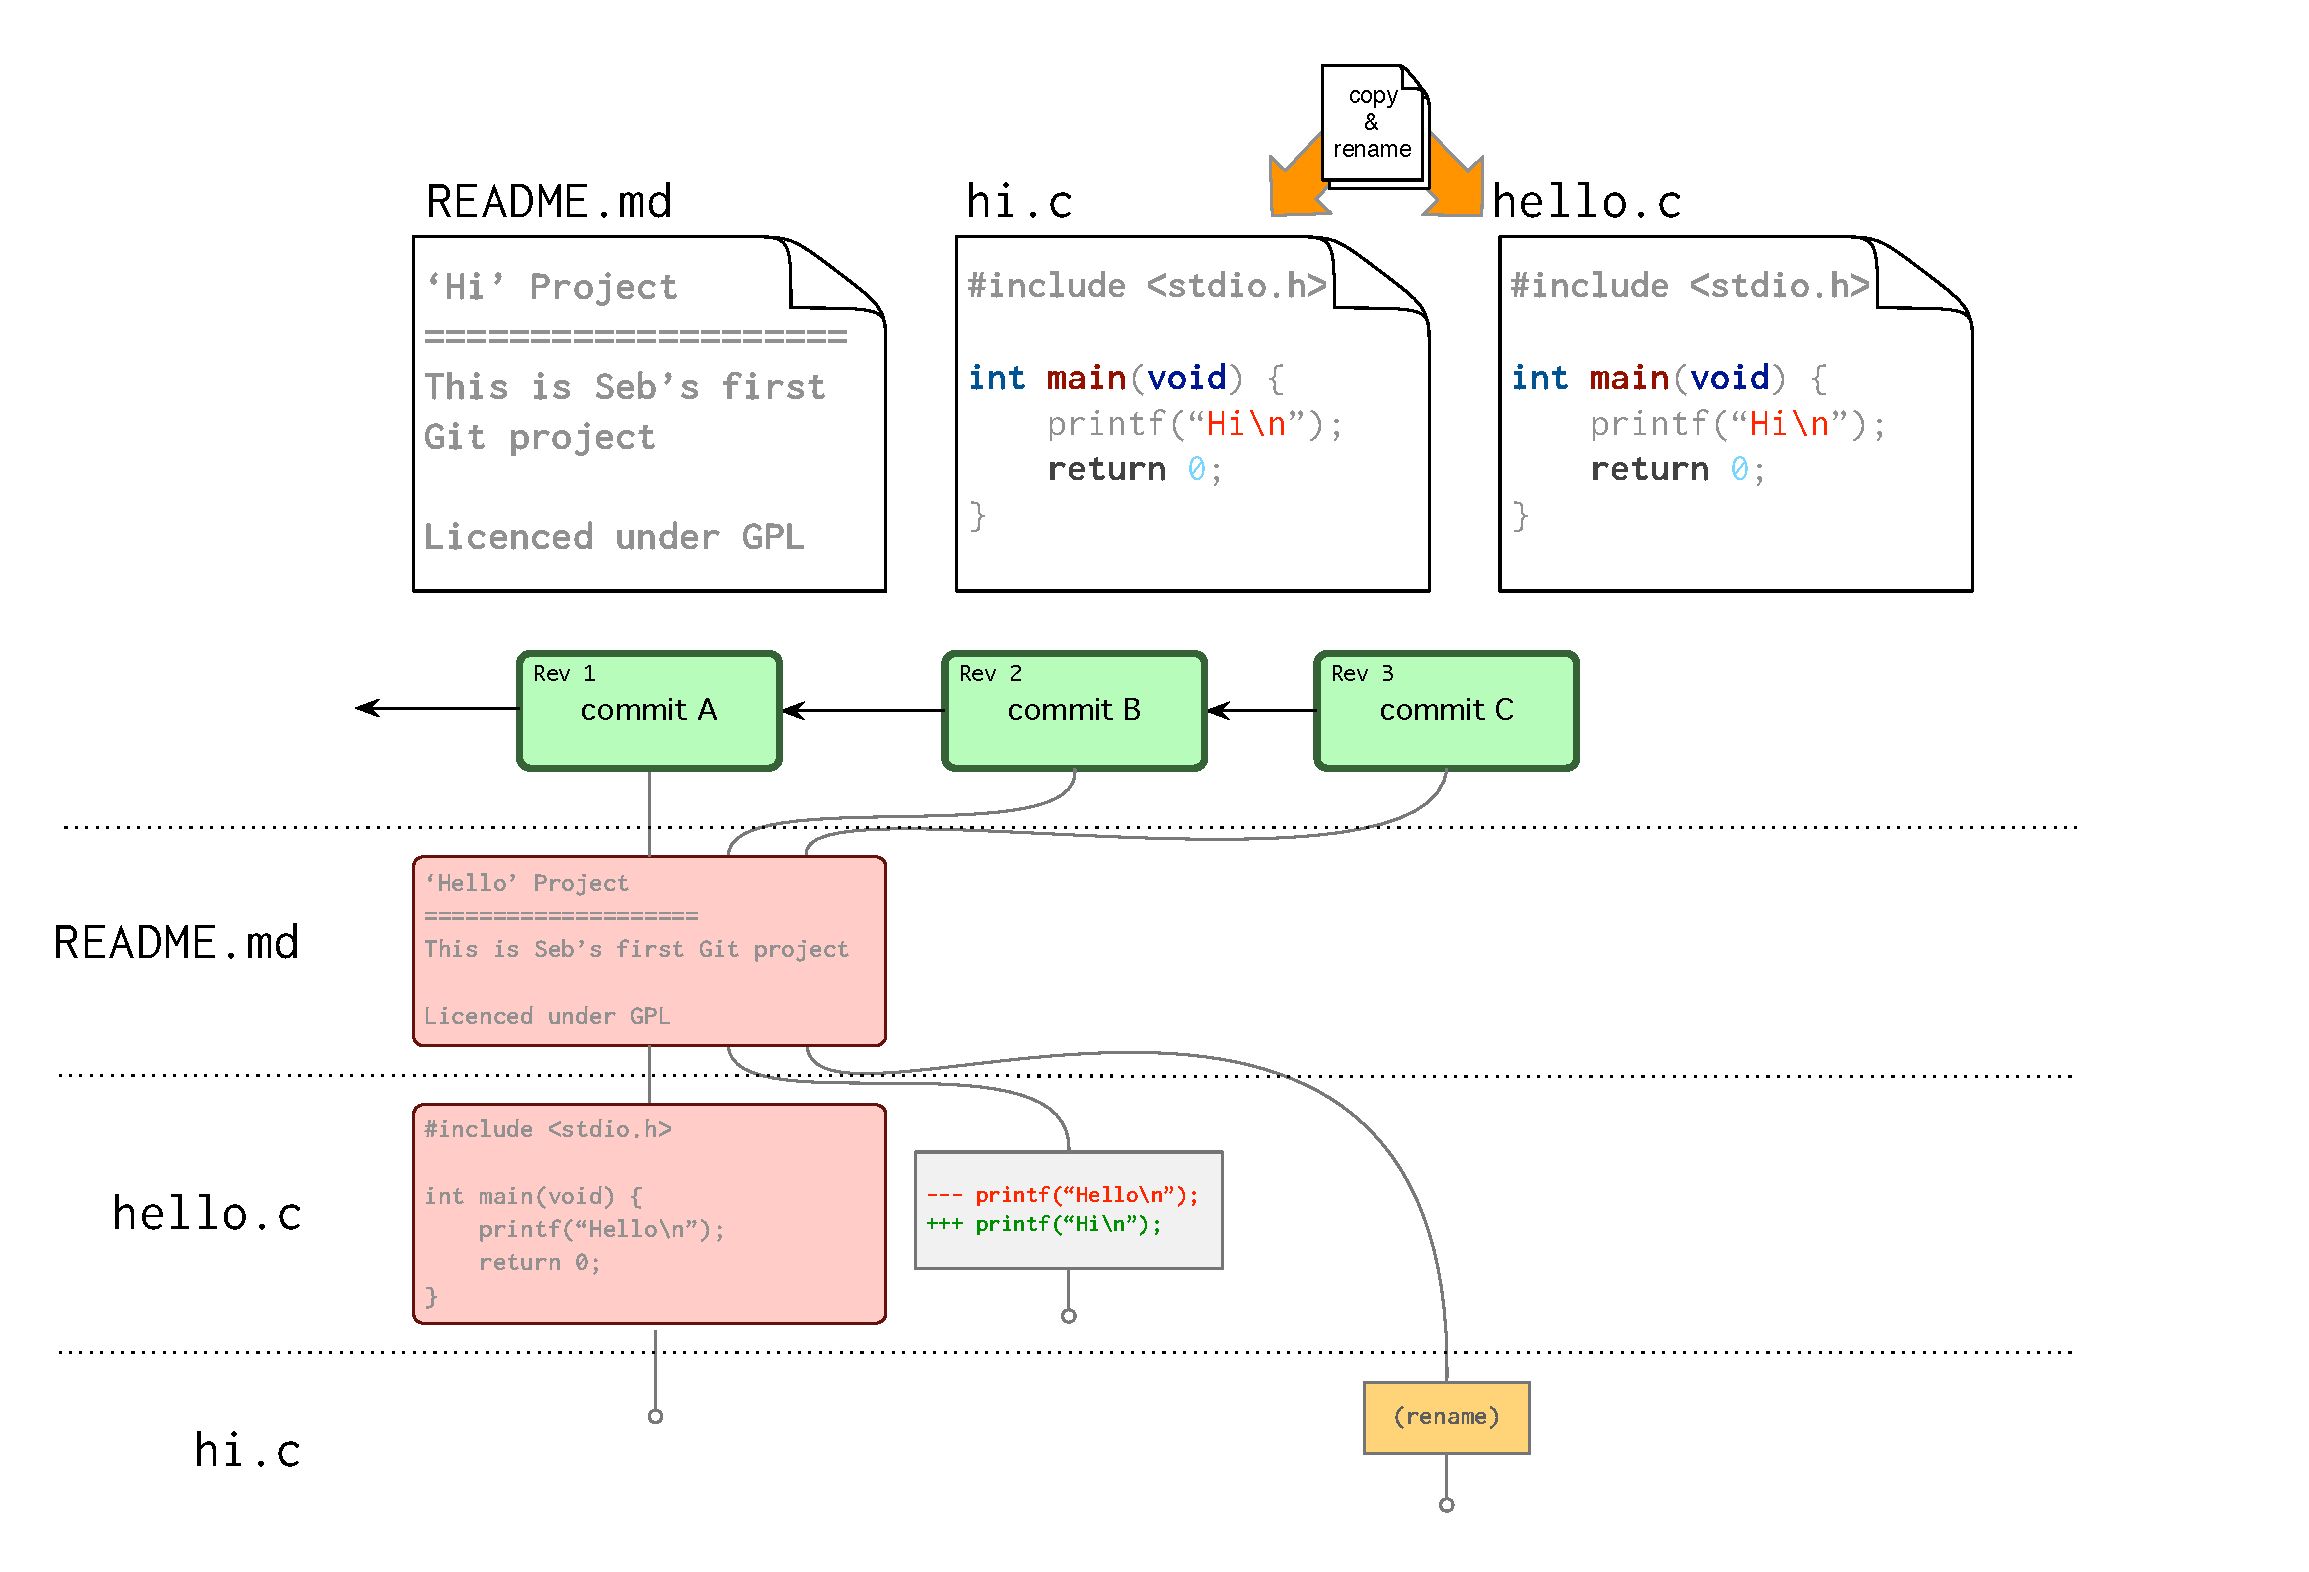
\includegraphics[height=0.95\textheight]{delta_vs_snapshot_example-012.pdf}}
  \only<13>{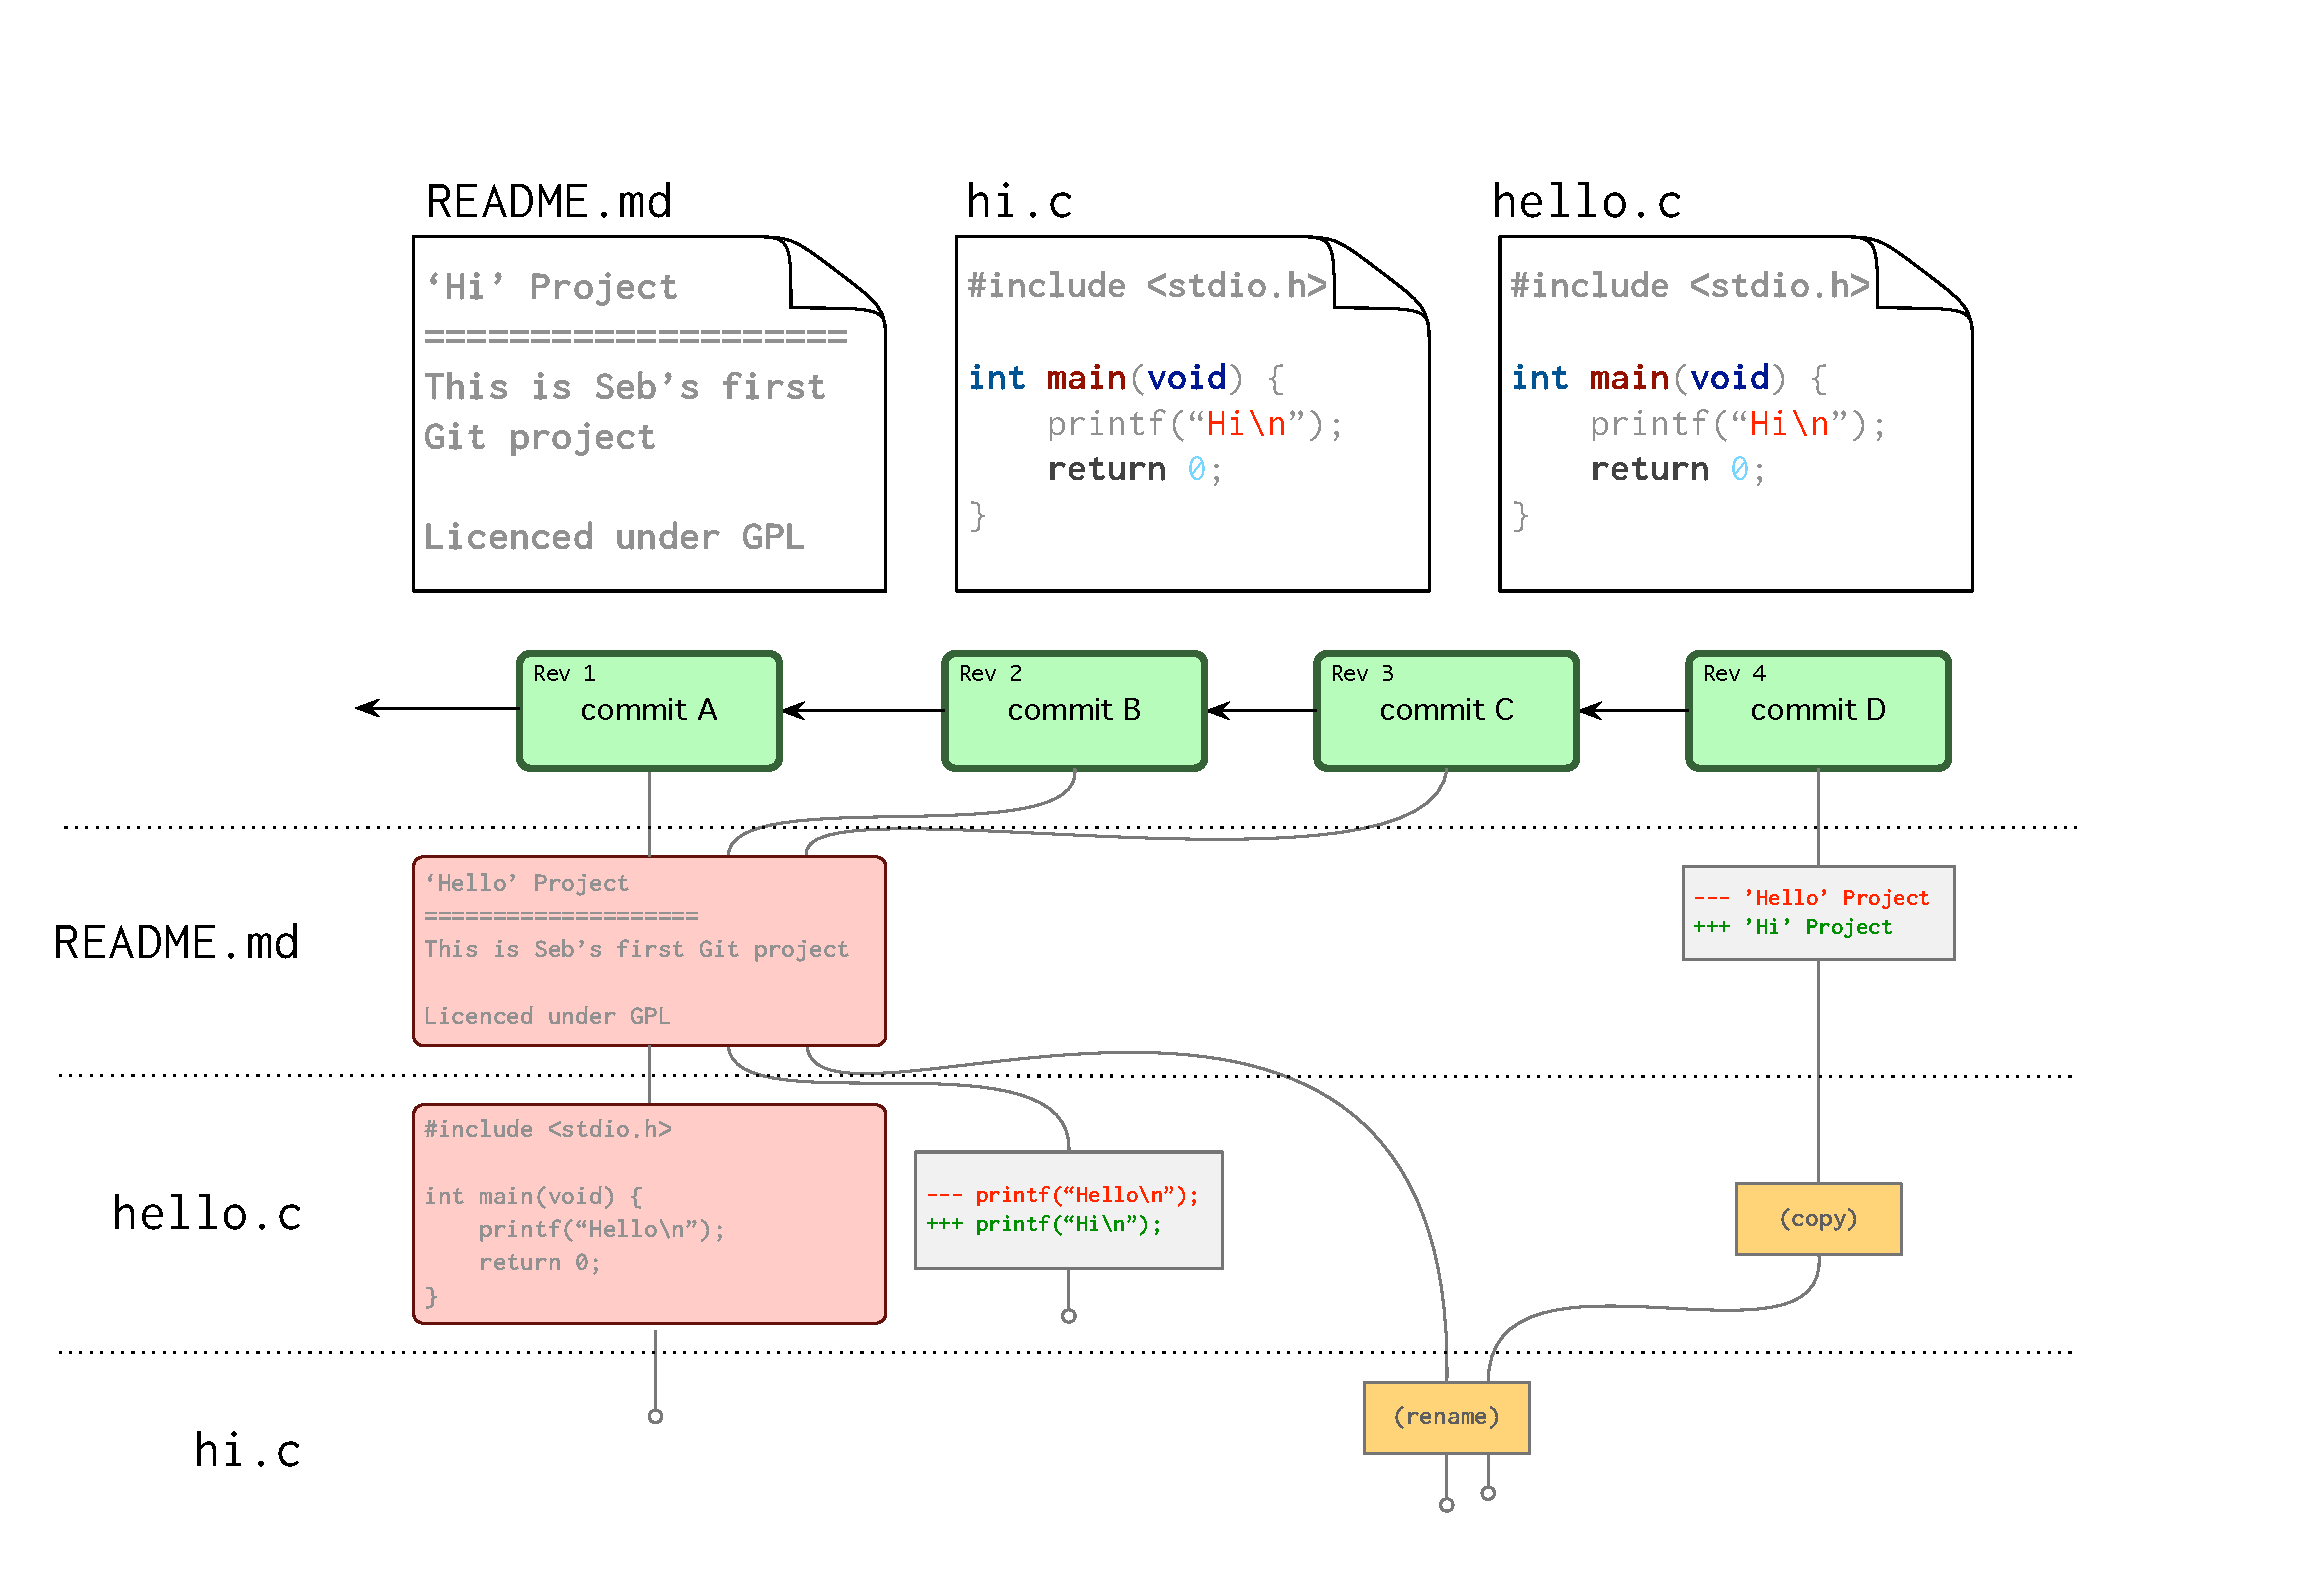
\includegraphics[height=0.95\textheight]{delta_vs_snapshot_example-013.pdf}}

}

% .......
\frame[t]{
  \frametitle{Git Snapshot (DAG) Storage}

  \vspace*{-1em}
  \only<1>{\includegraphics [height=0.95\textheight]{delta_vs_snapshot_example-101.pdf}}
  \only<2>{\includegraphics [height=0.95\textheight]{delta_vs_snapshot_example-102.pdf}}
  \only<3>{\includegraphics [height=0.95\textheight]{delta_vs_snapshot_example-103.pdf}}
  \only<4>{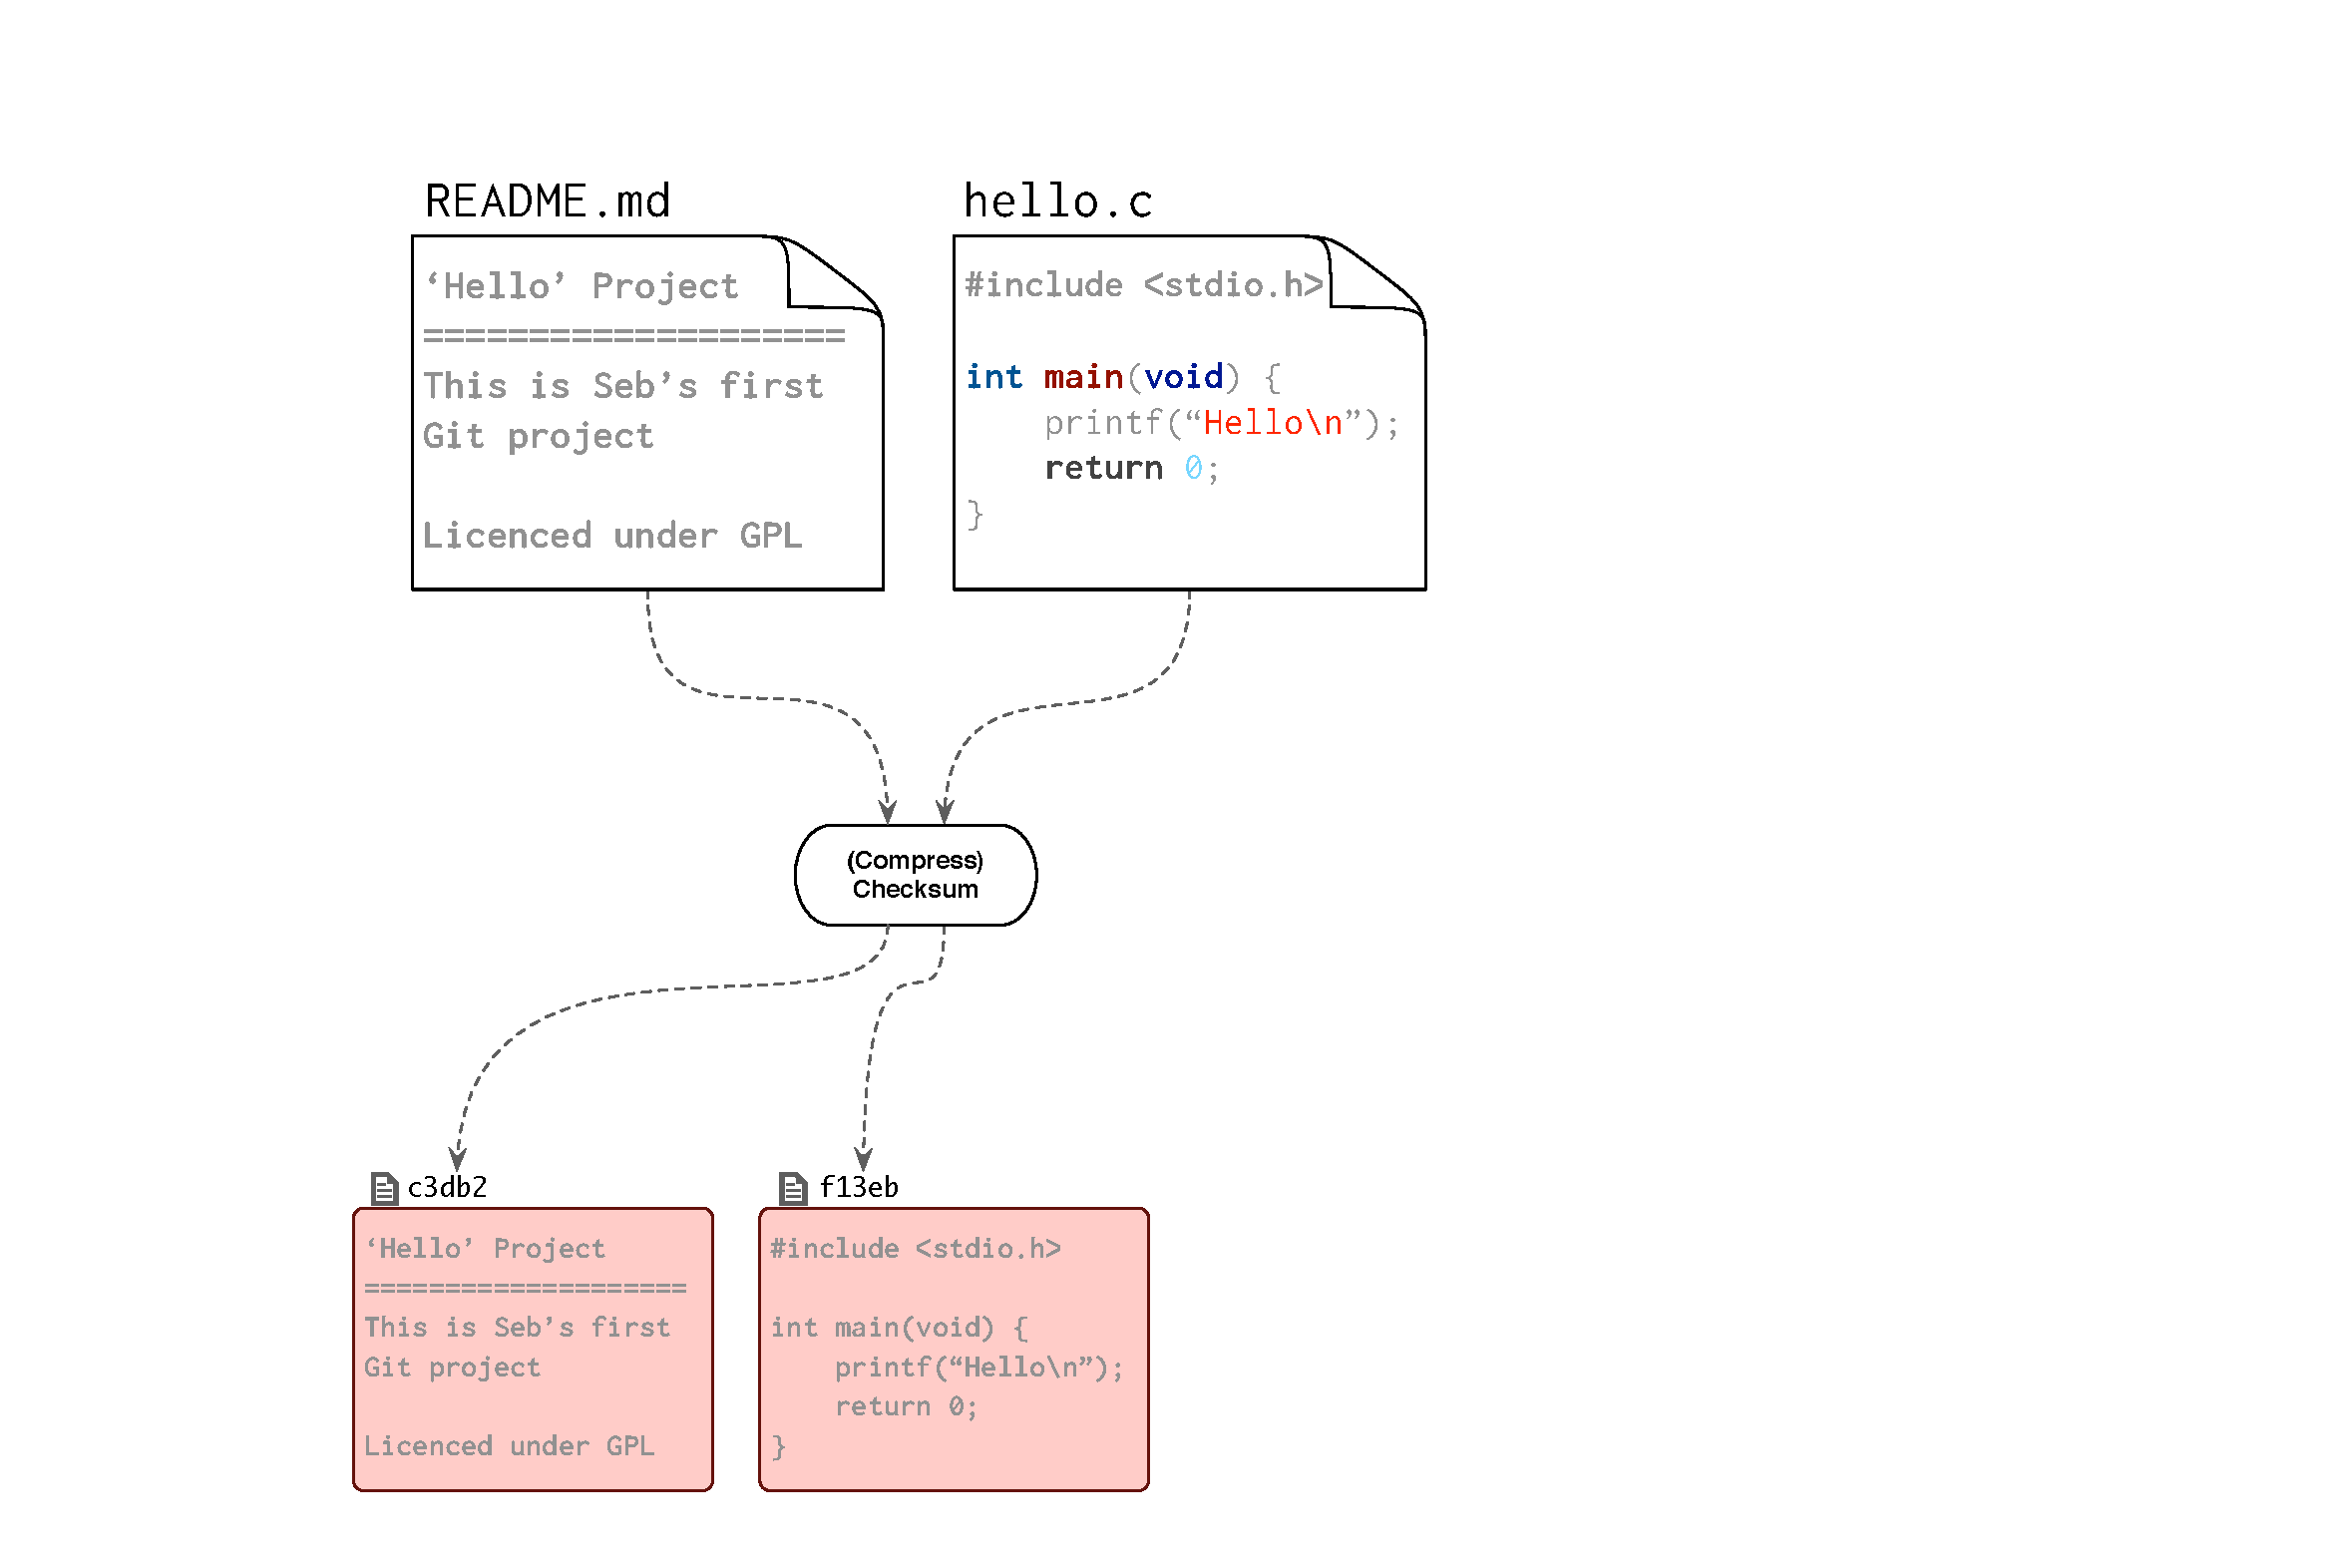
\includegraphics [height=0.95\textheight]{delta_vs_snapshot_example-104.pdf}}
  \only<5>{\includegraphics [height=0.95\textheight]{delta_vs_snapshot_example-105.pdf}}
  \only<6>{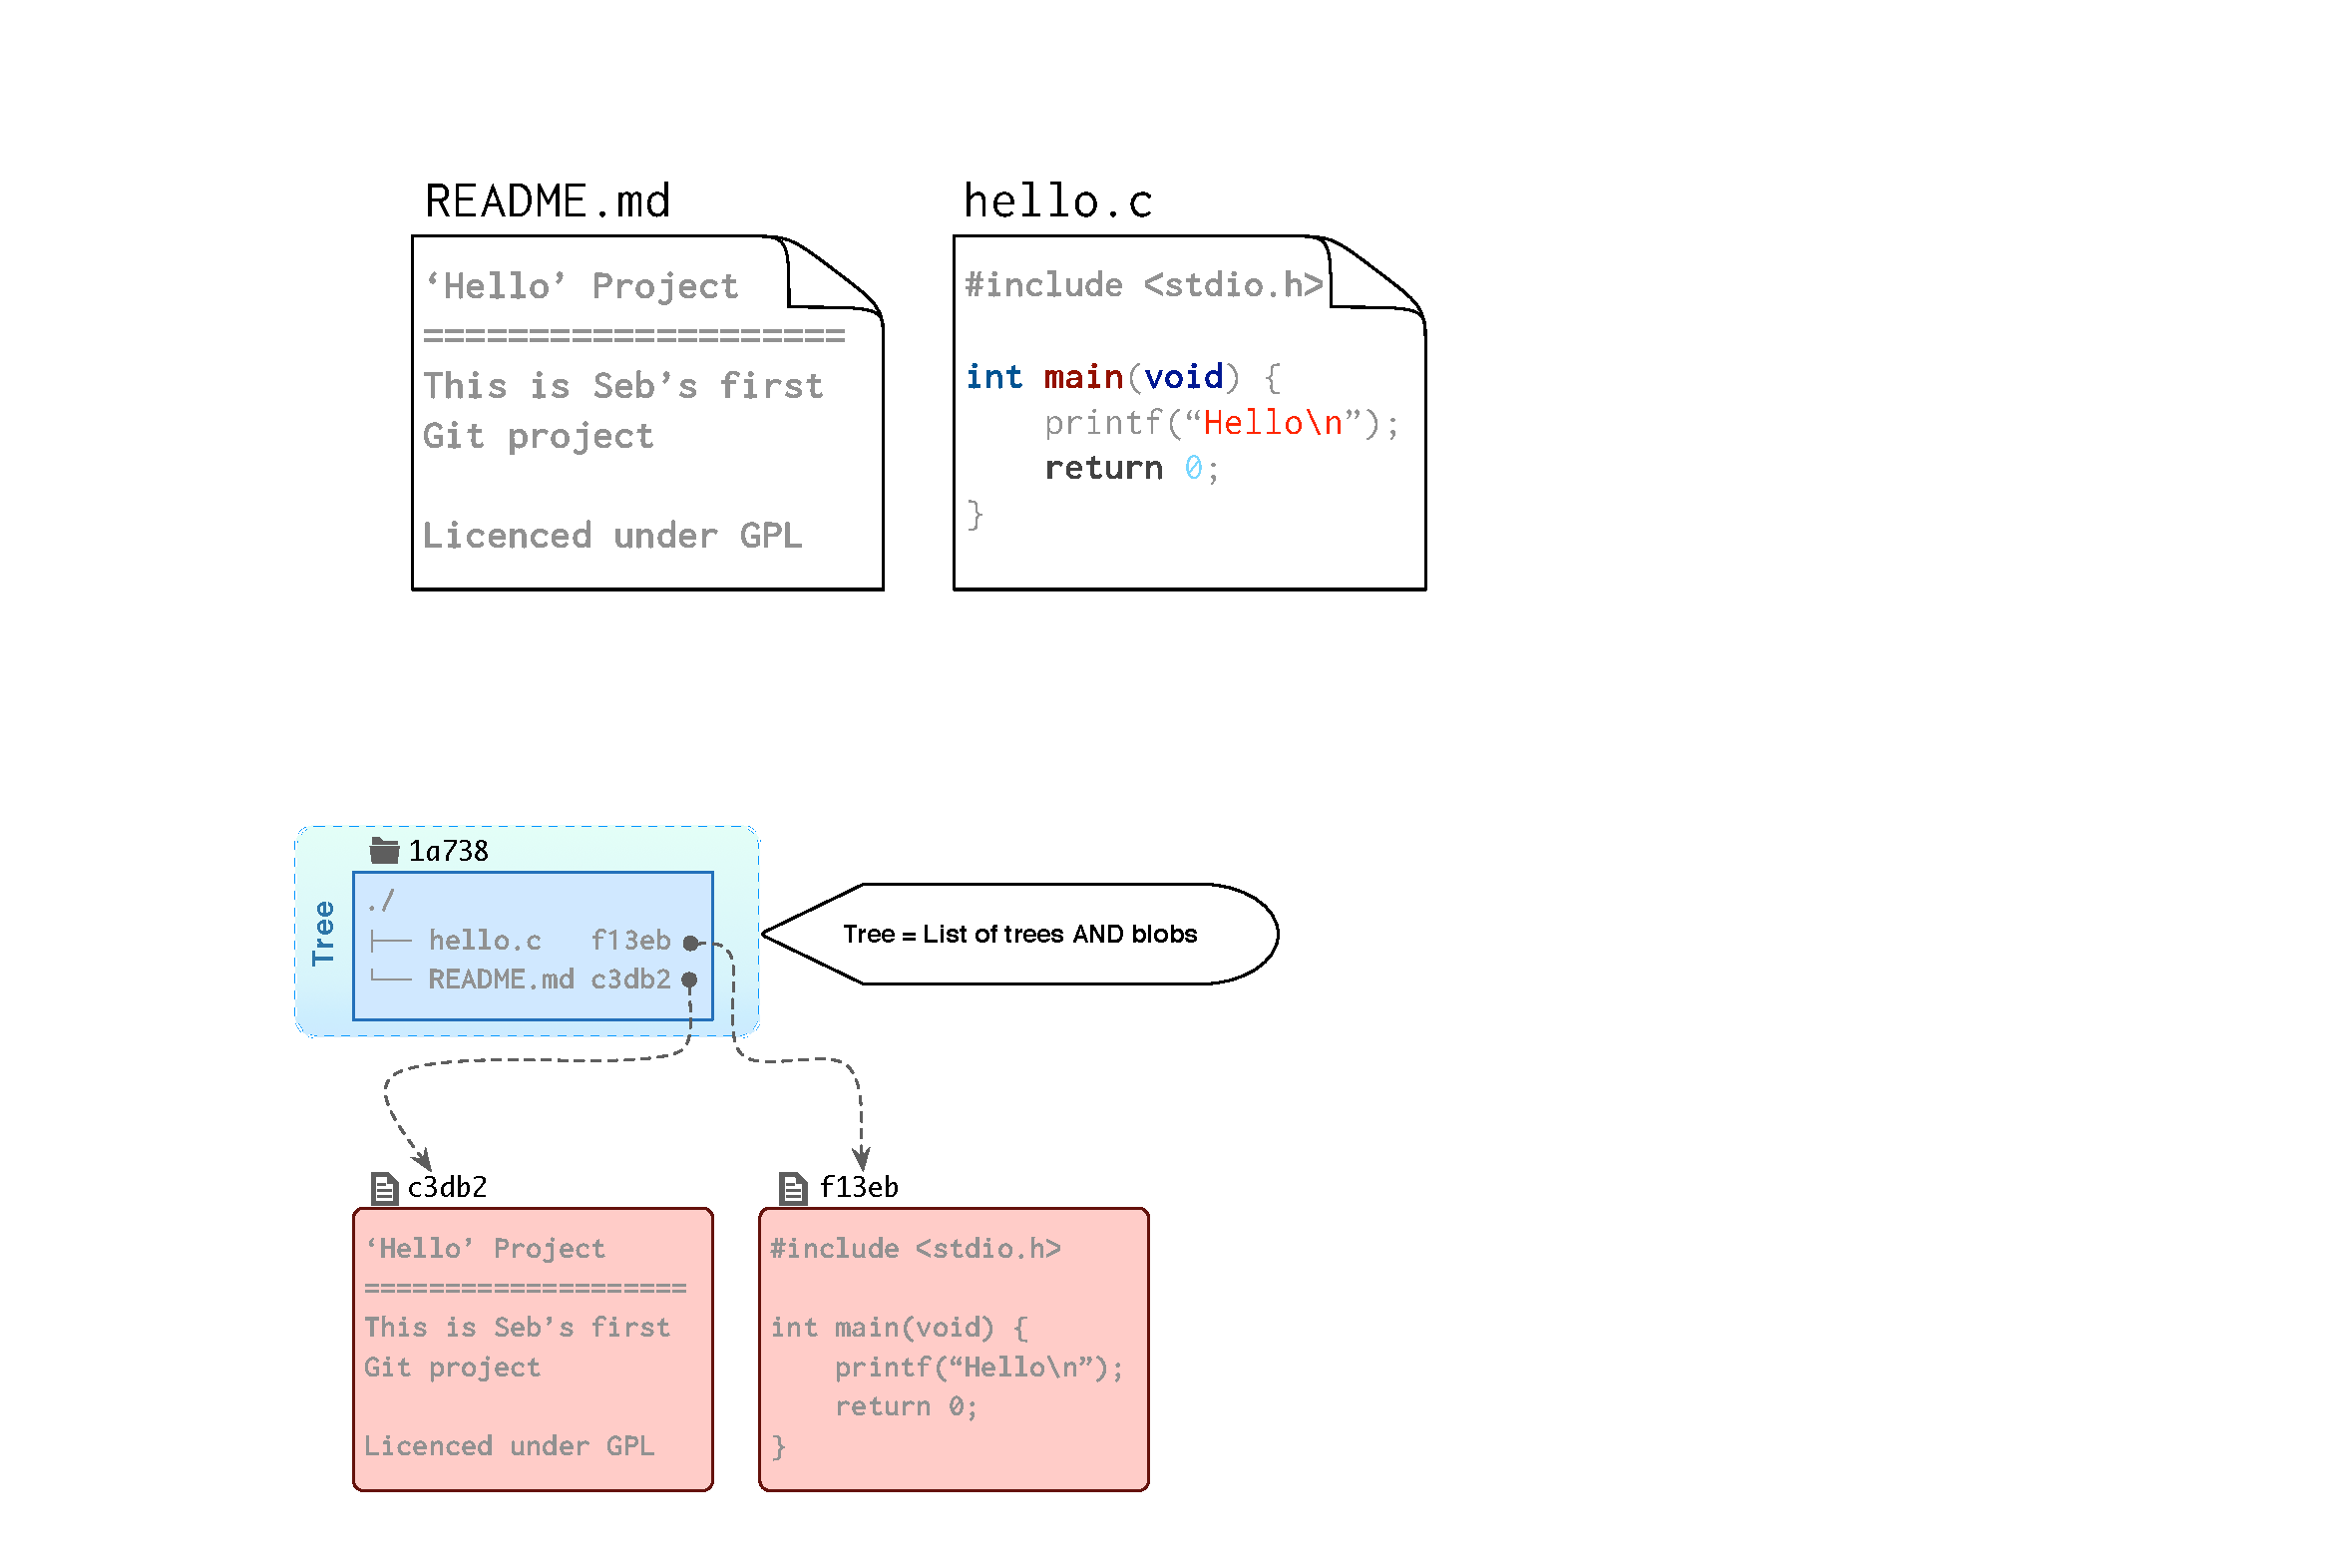
\includegraphics [height=0.95\textheight]{delta_vs_snapshot_example-106.pdf}}
  \only<7>{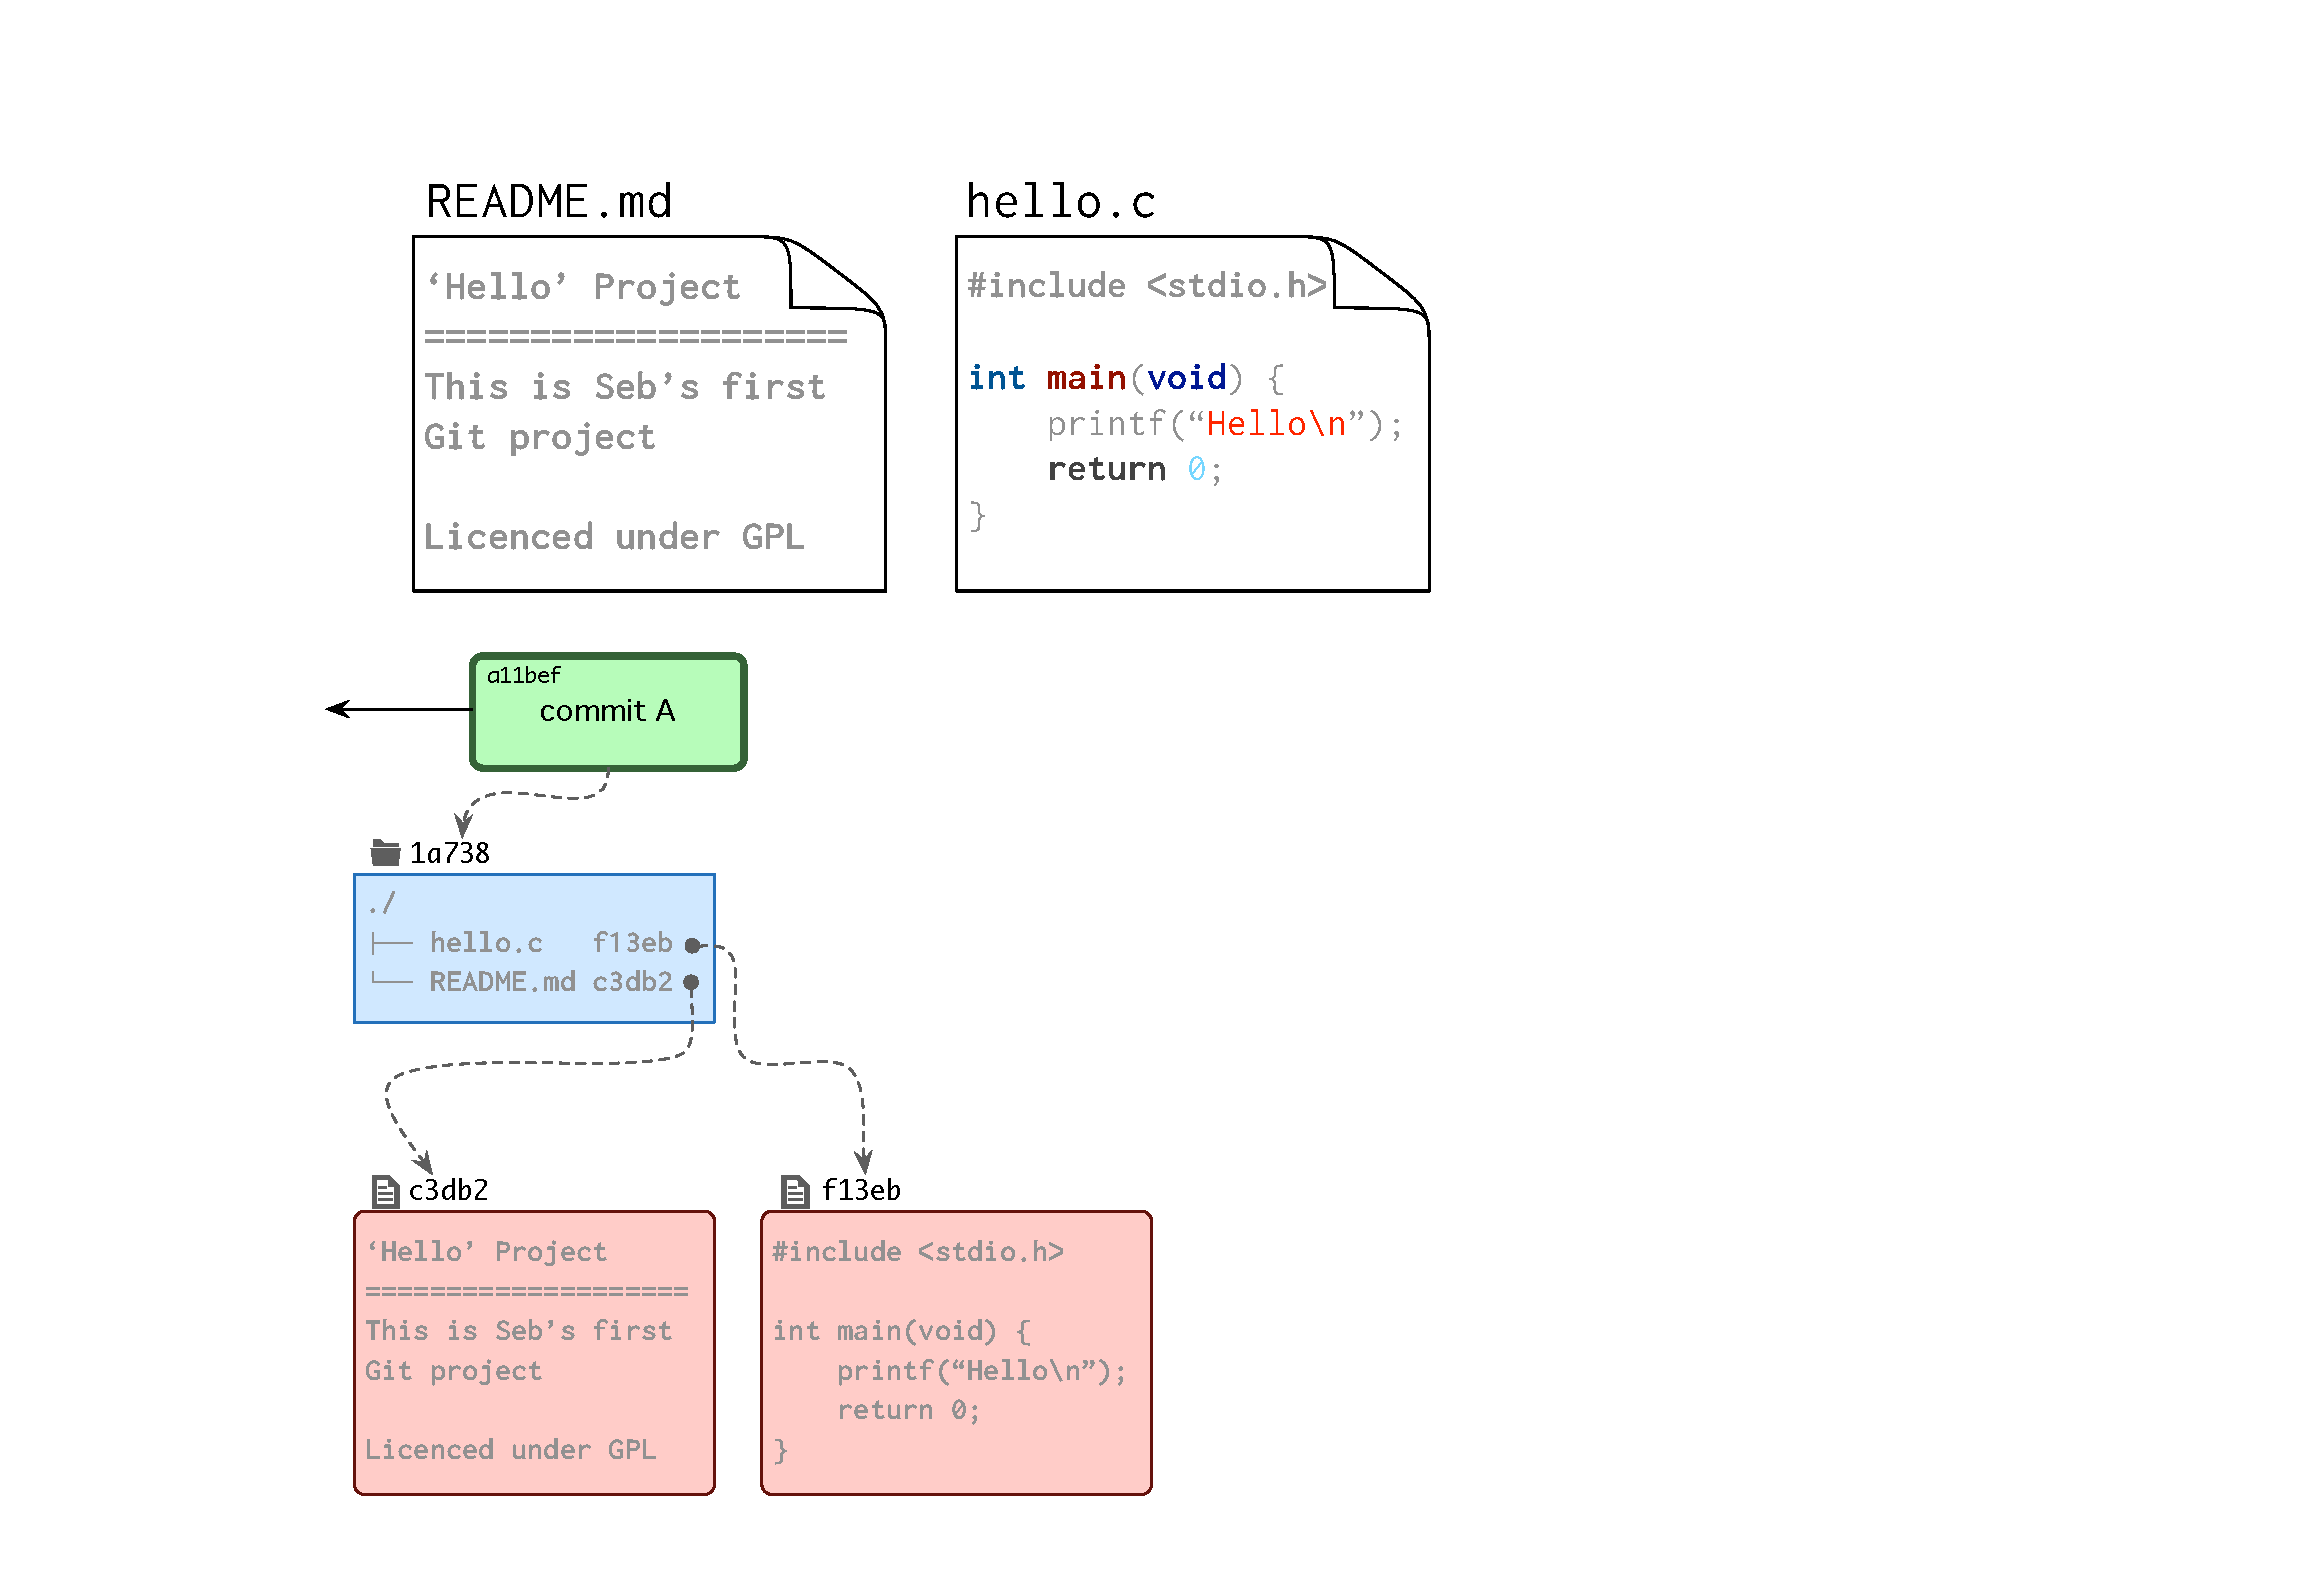
\includegraphics [height=0.95\textheight]{delta_vs_snapshot_example-107.pdf}}
  \only<8>{\includegraphics [height=0.95\textheight]{delta_vs_snapshot_example-108.pdf}}
  \only<9>{\includegraphics [height=0.95\textheight]{delta_vs_snapshot_example-109.pdf}}
  \only<10>{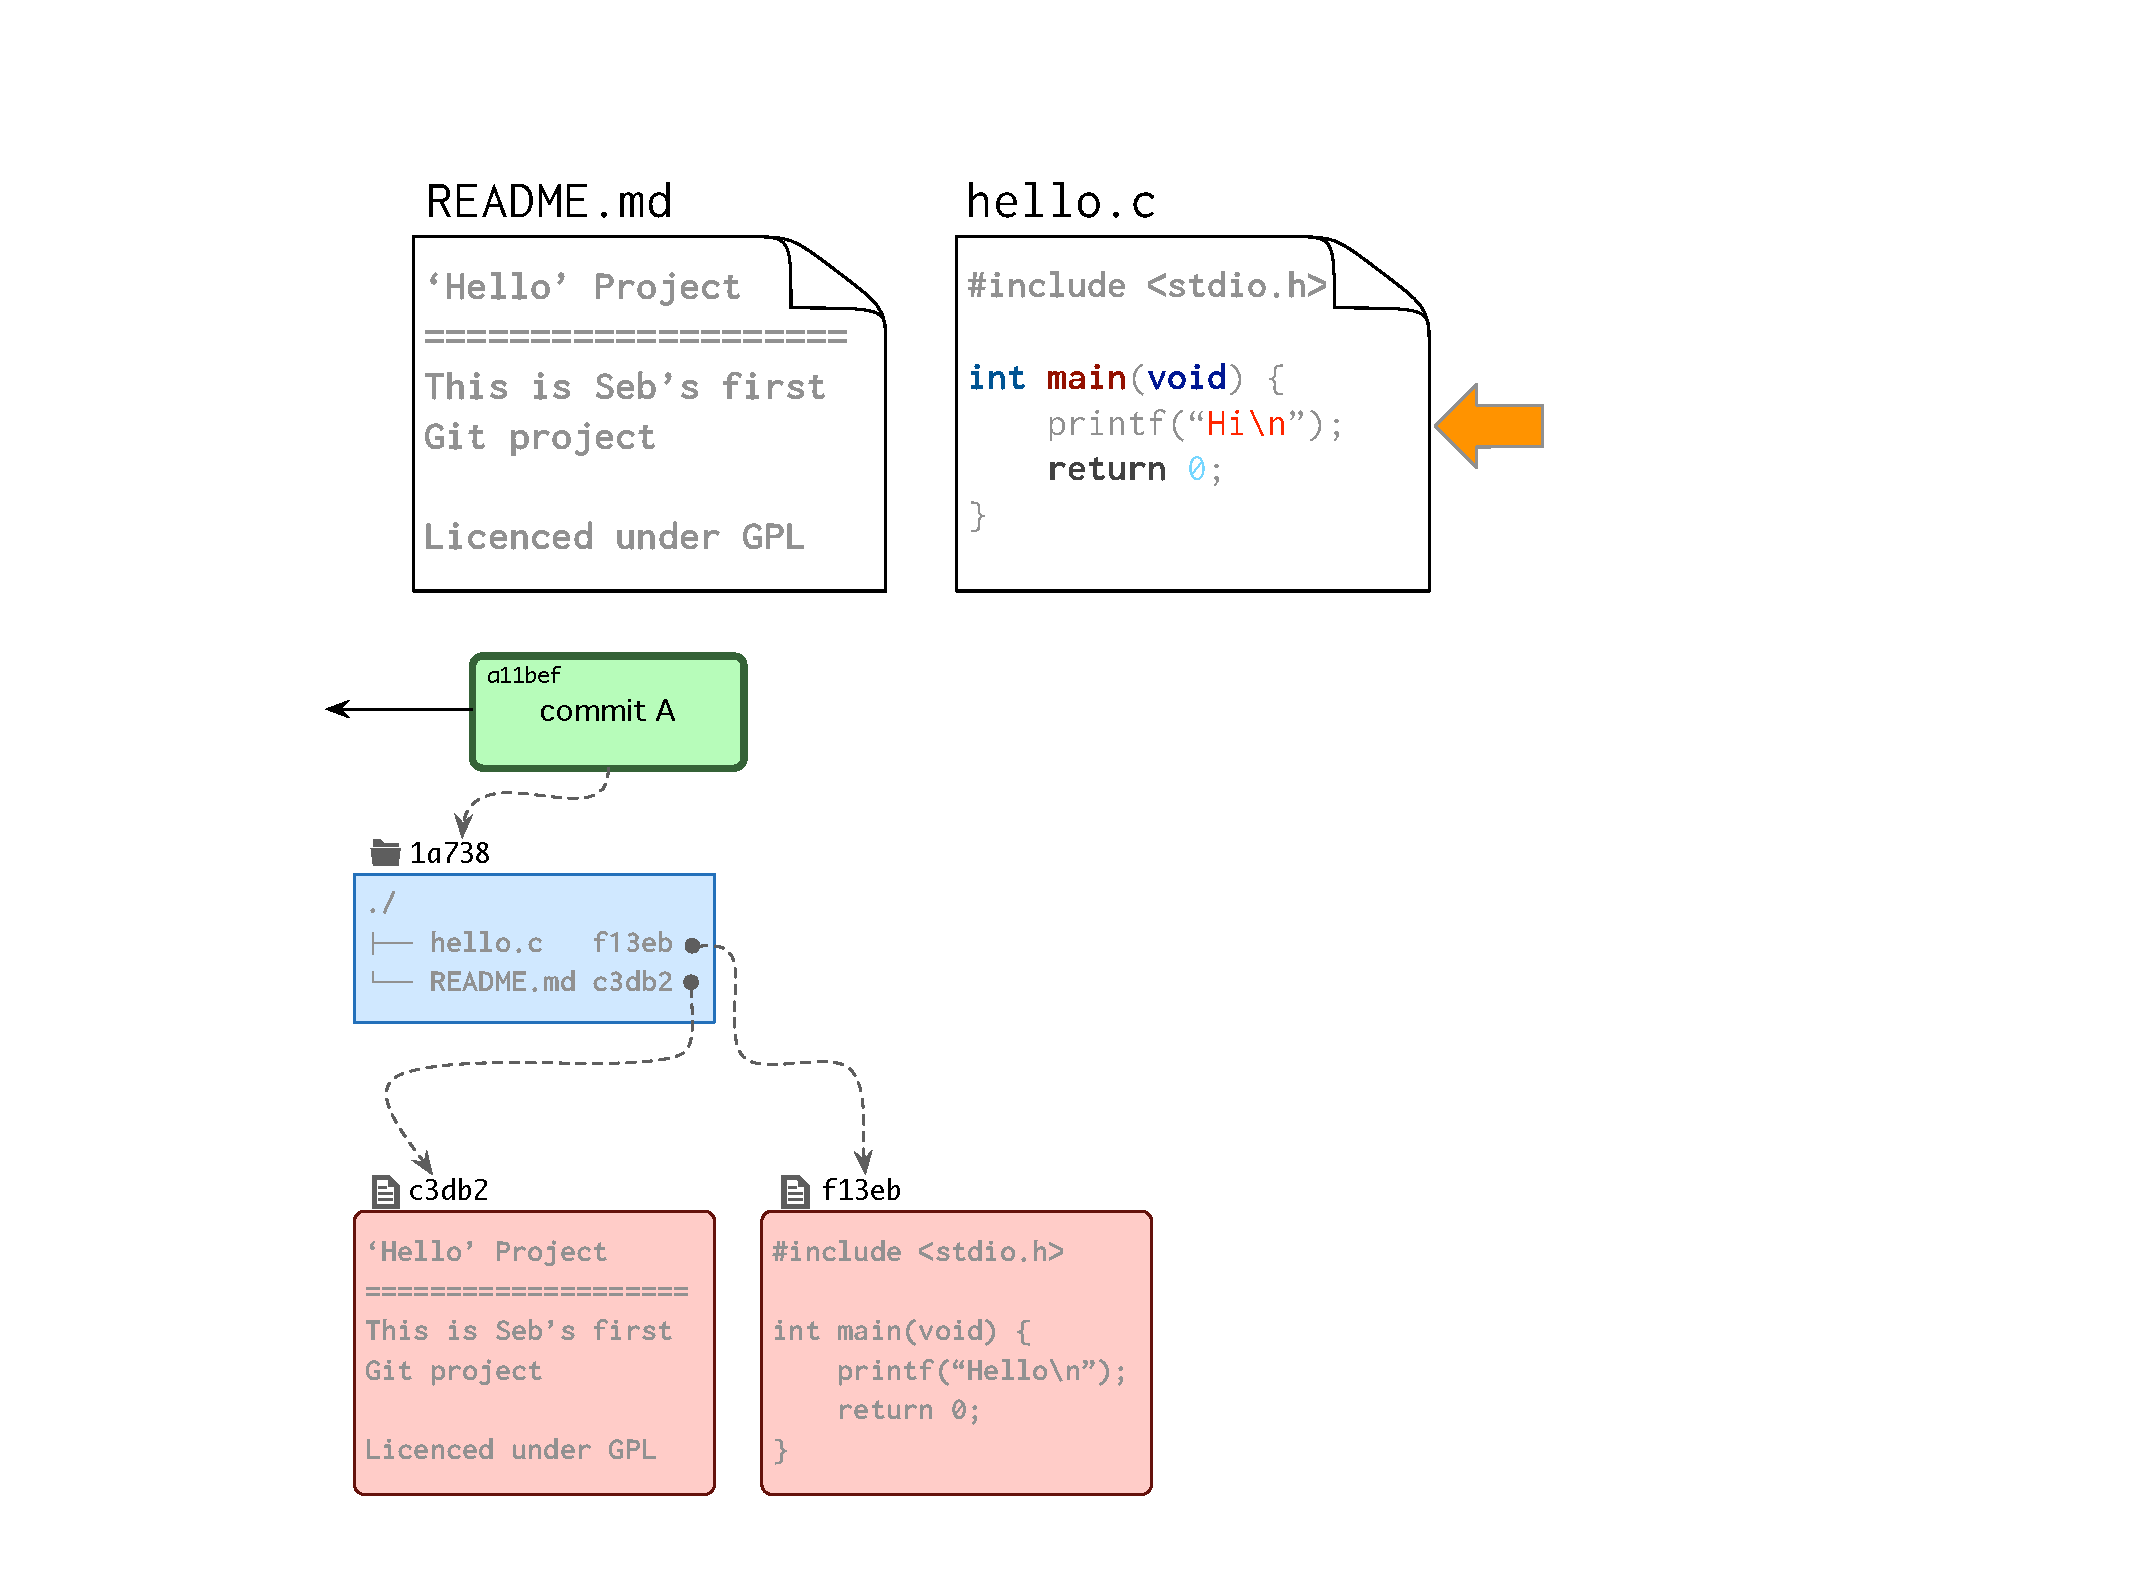
\includegraphics[height=0.95\textheight]{delta_vs_snapshot_example-110.pdf}}
  \only<11>{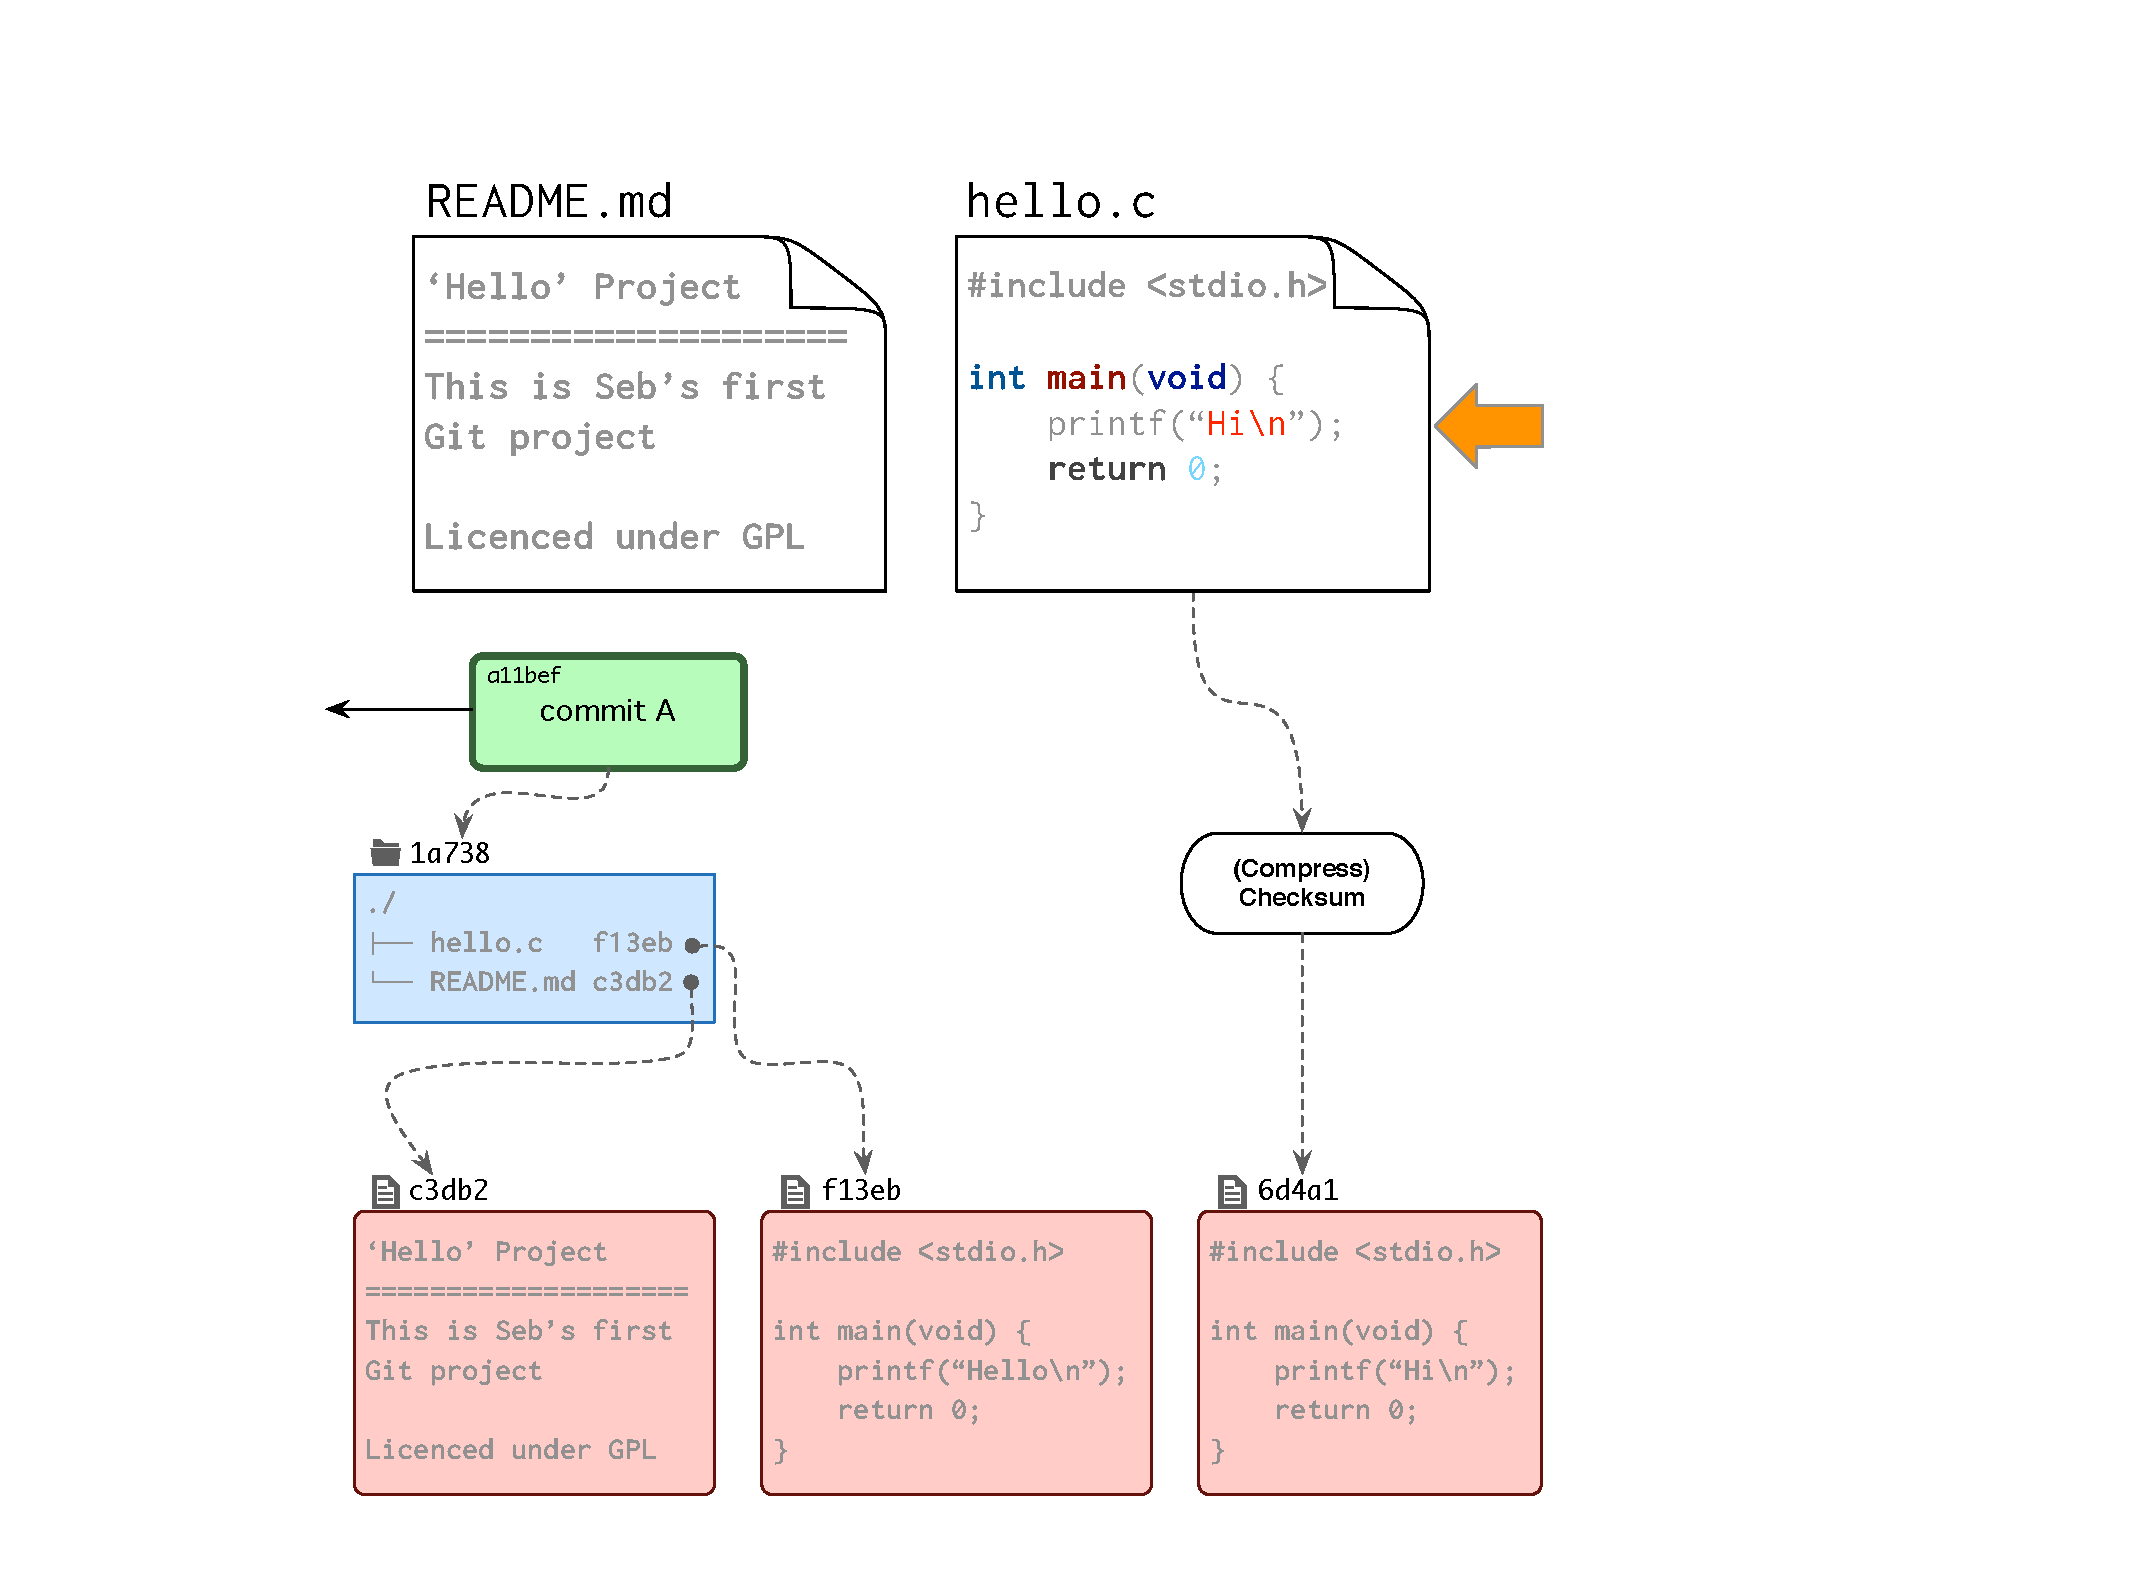
\includegraphics[height=0.95\textheight]{delta_vs_snapshot_example-111.pdf}}
  \only<12>{\includegraphics[height=0.95\textheight]{delta_vs_snapshot_example-112.pdf}}
  \only<13>{\includegraphics[height=0.95\textheight]{delta_vs_snapshot_example-113.pdf}}
  \only<14>{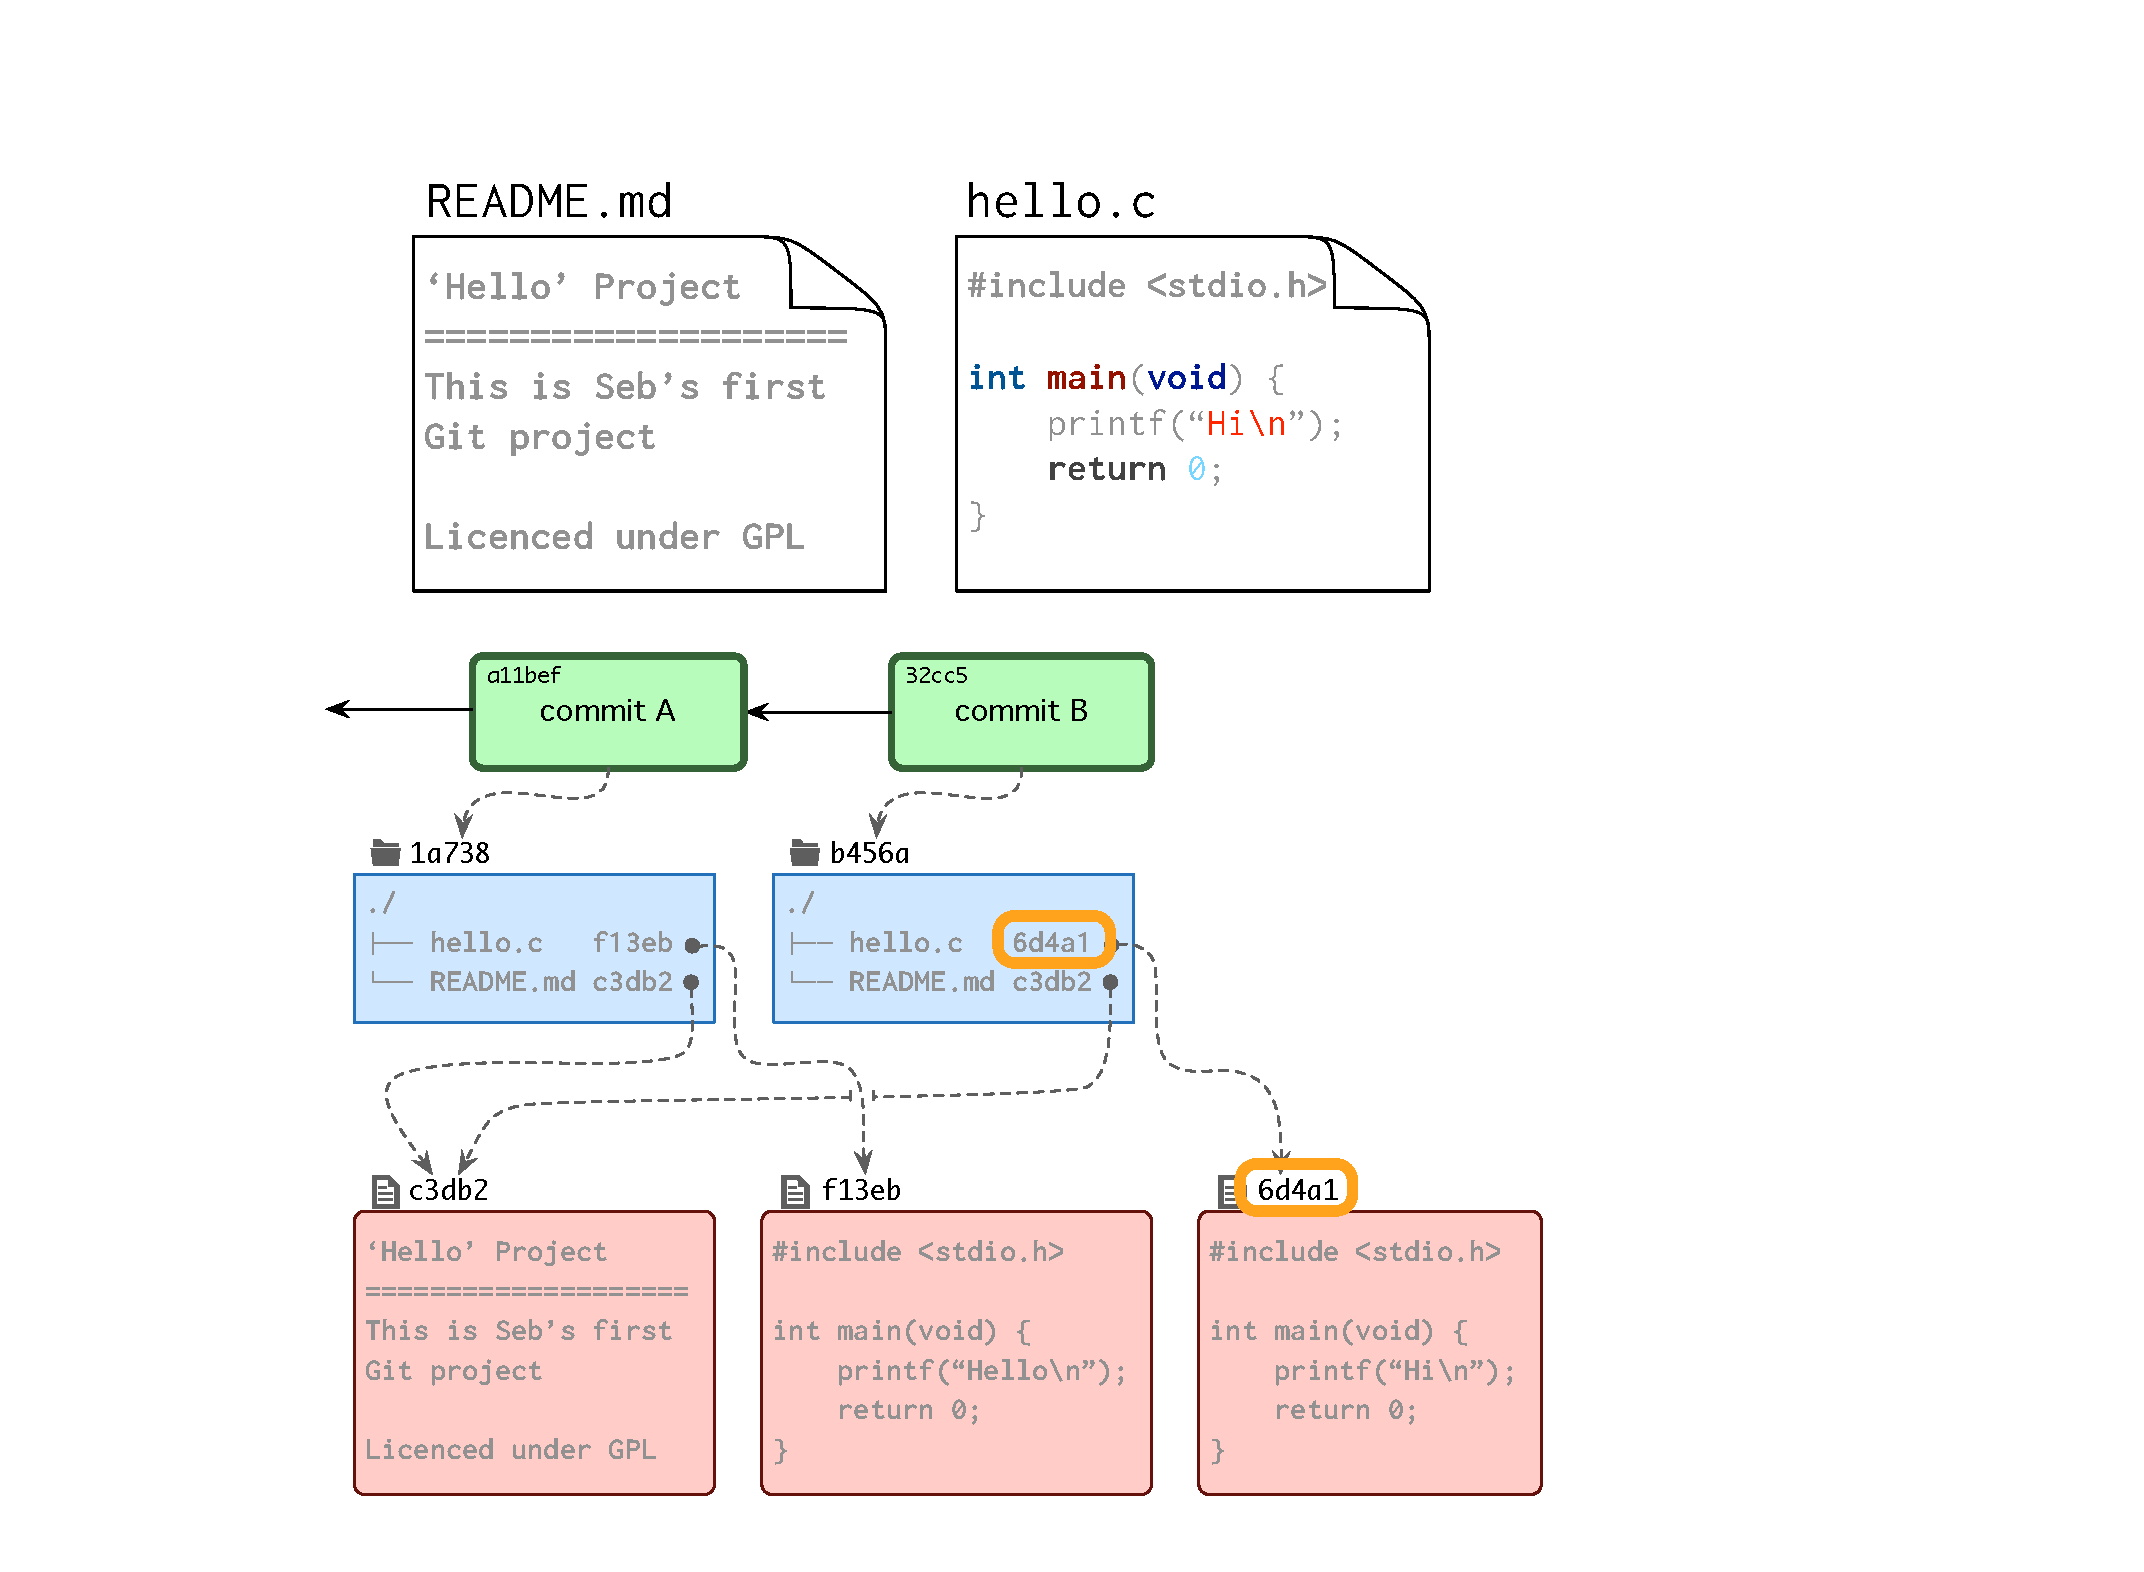
\includegraphics[height=0.95\textheight]{delta_vs_snapshot_example-114.pdf}}
  \only<15>{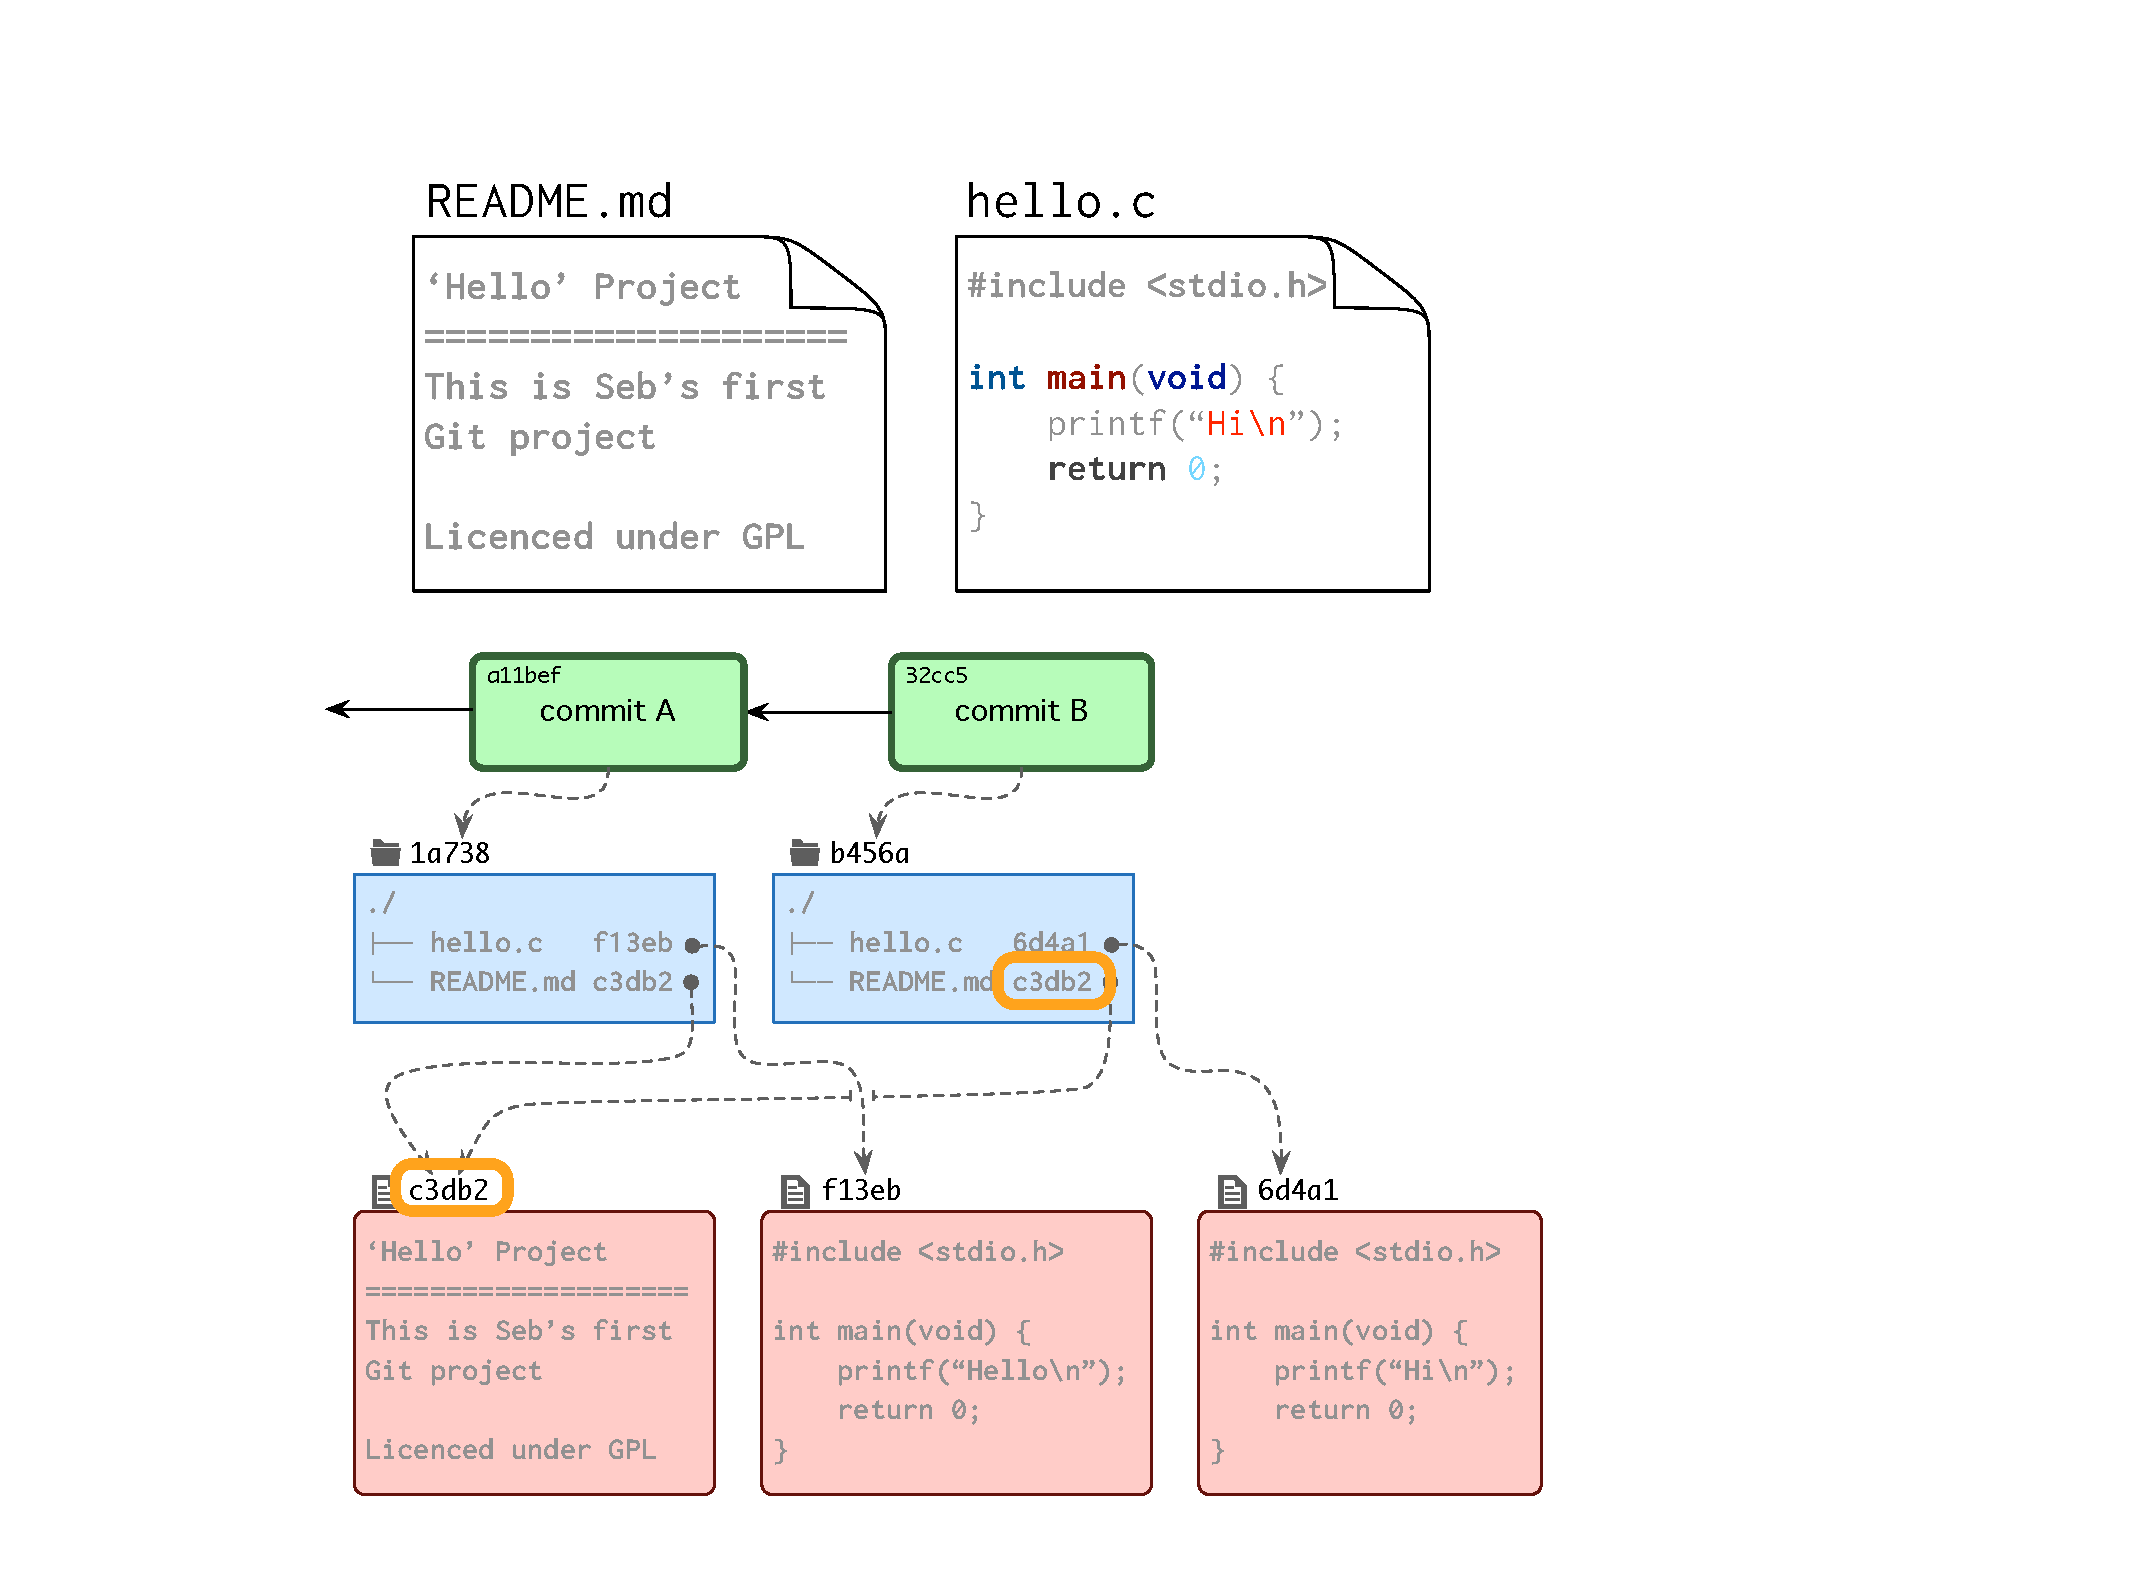
\includegraphics[height=0.95\textheight]{delta_vs_snapshot_example-115.pdf}}
  \only<16>{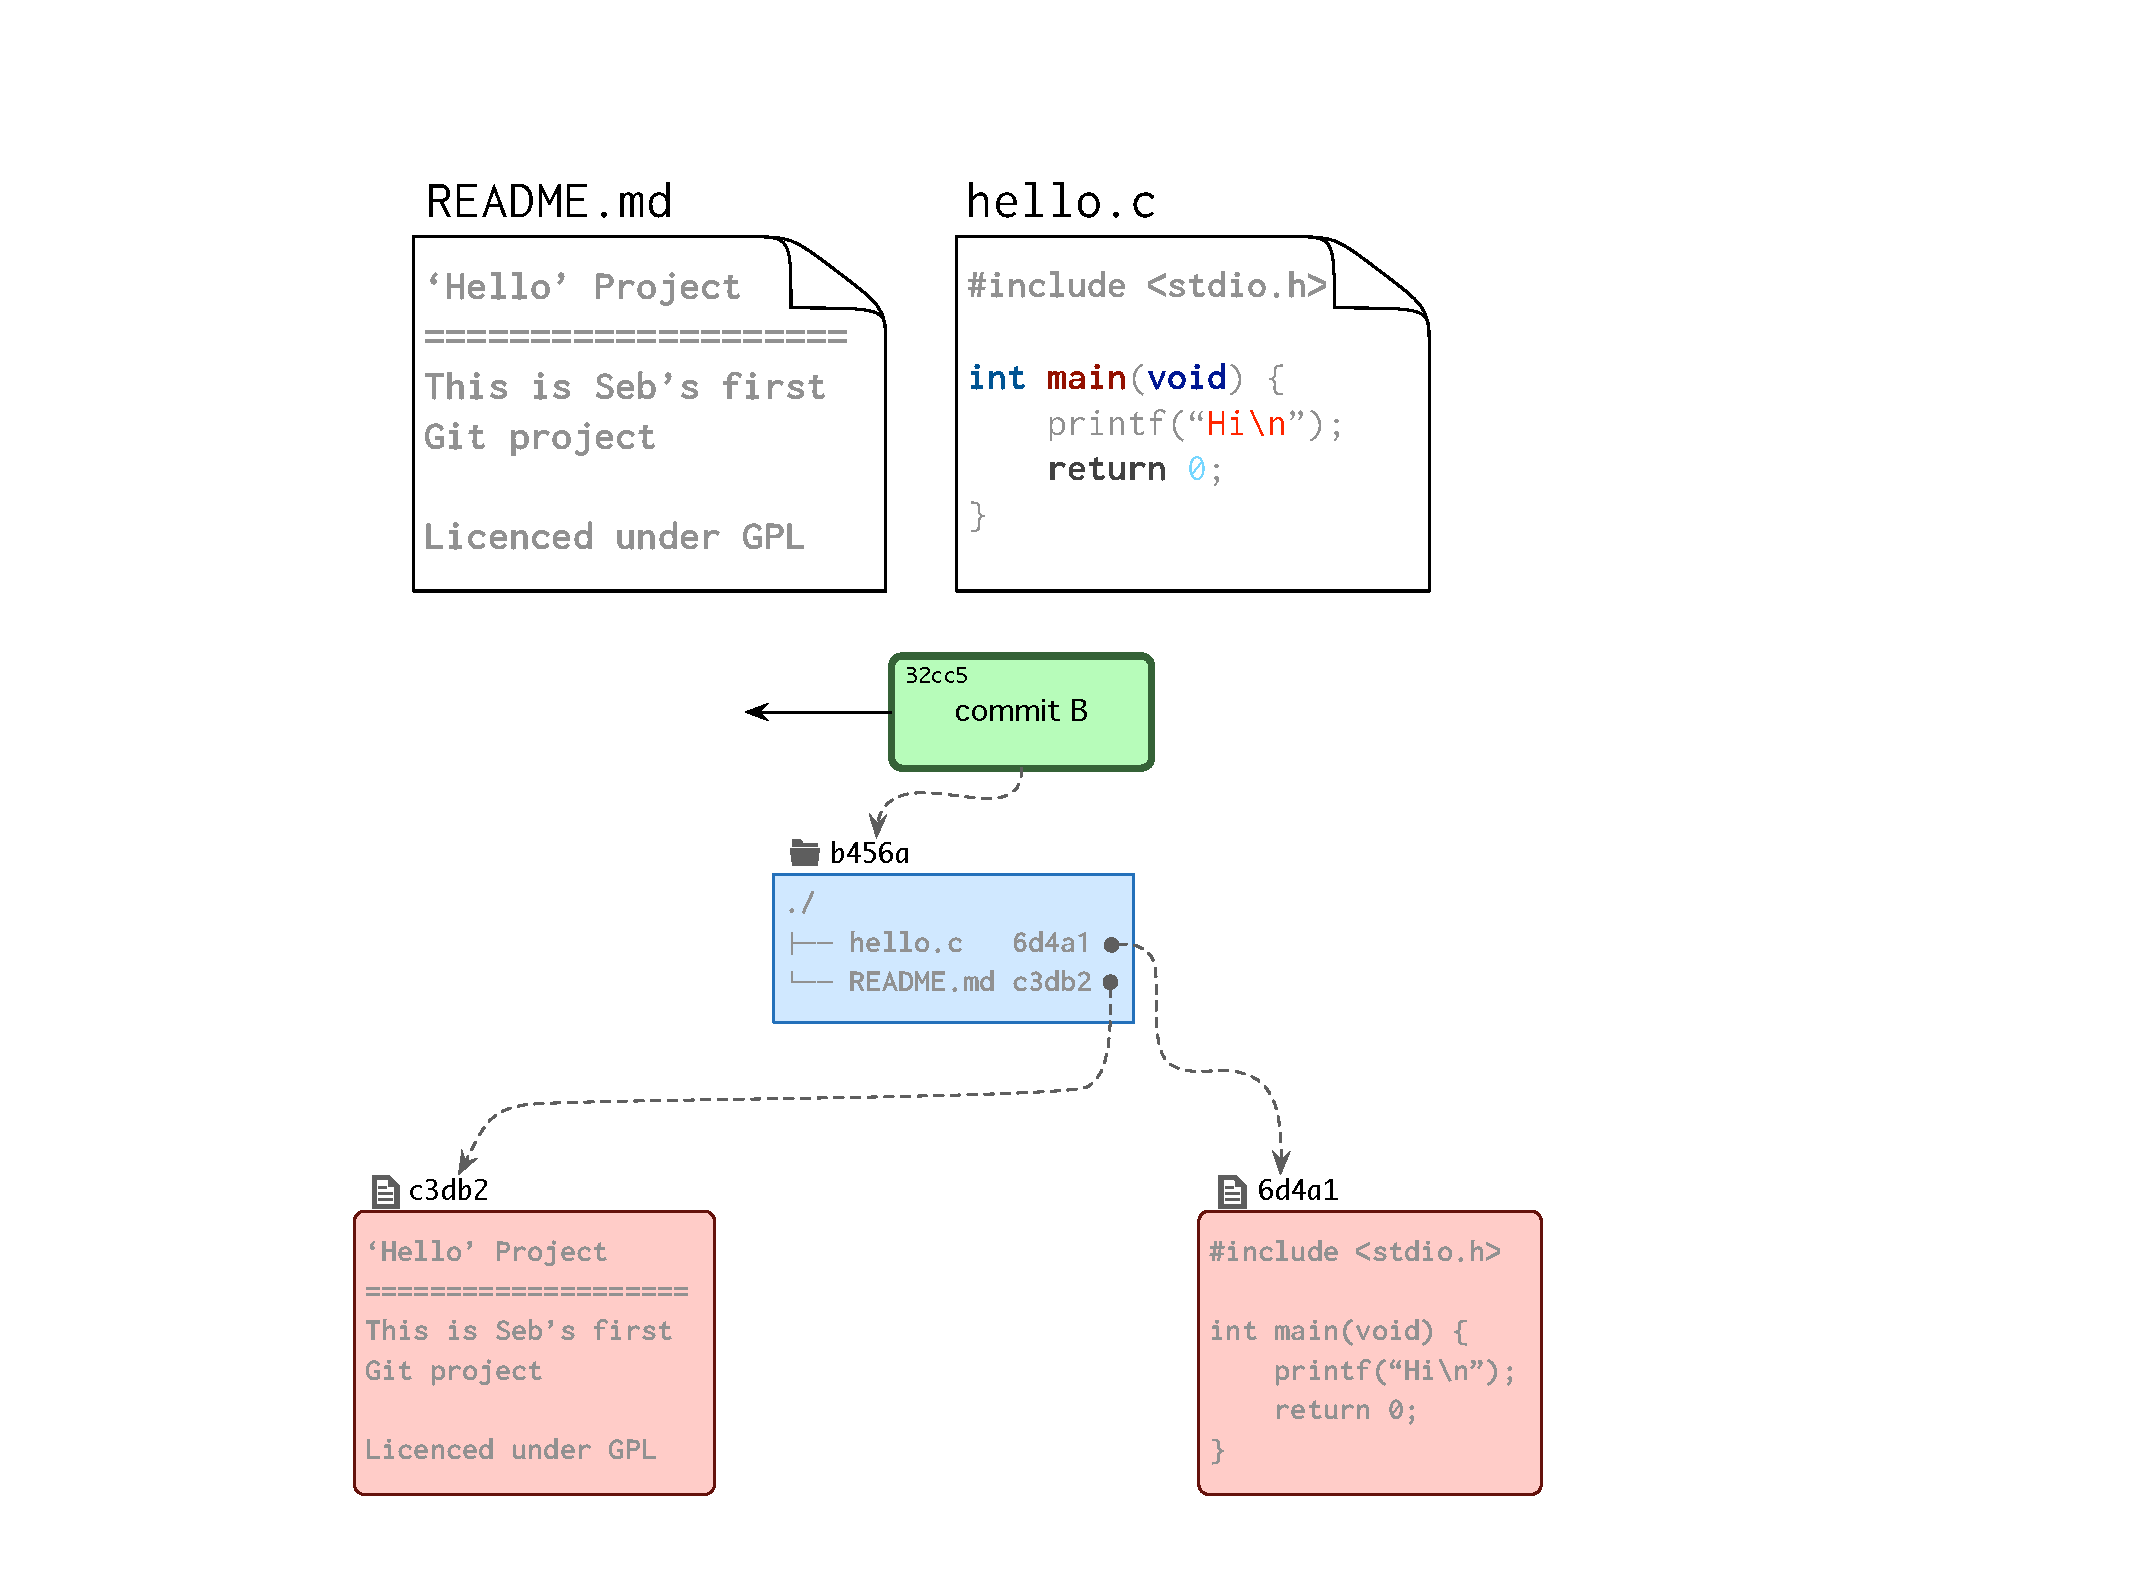
\includegraphics[height=0.95\textheight]{delta_vs_snapshot_example-116.pdf}}
  \only<17>{\includegraphics[height=0.95\textheight]{delta_vs_snapshot_example-117.pdf}}
  \only<18>{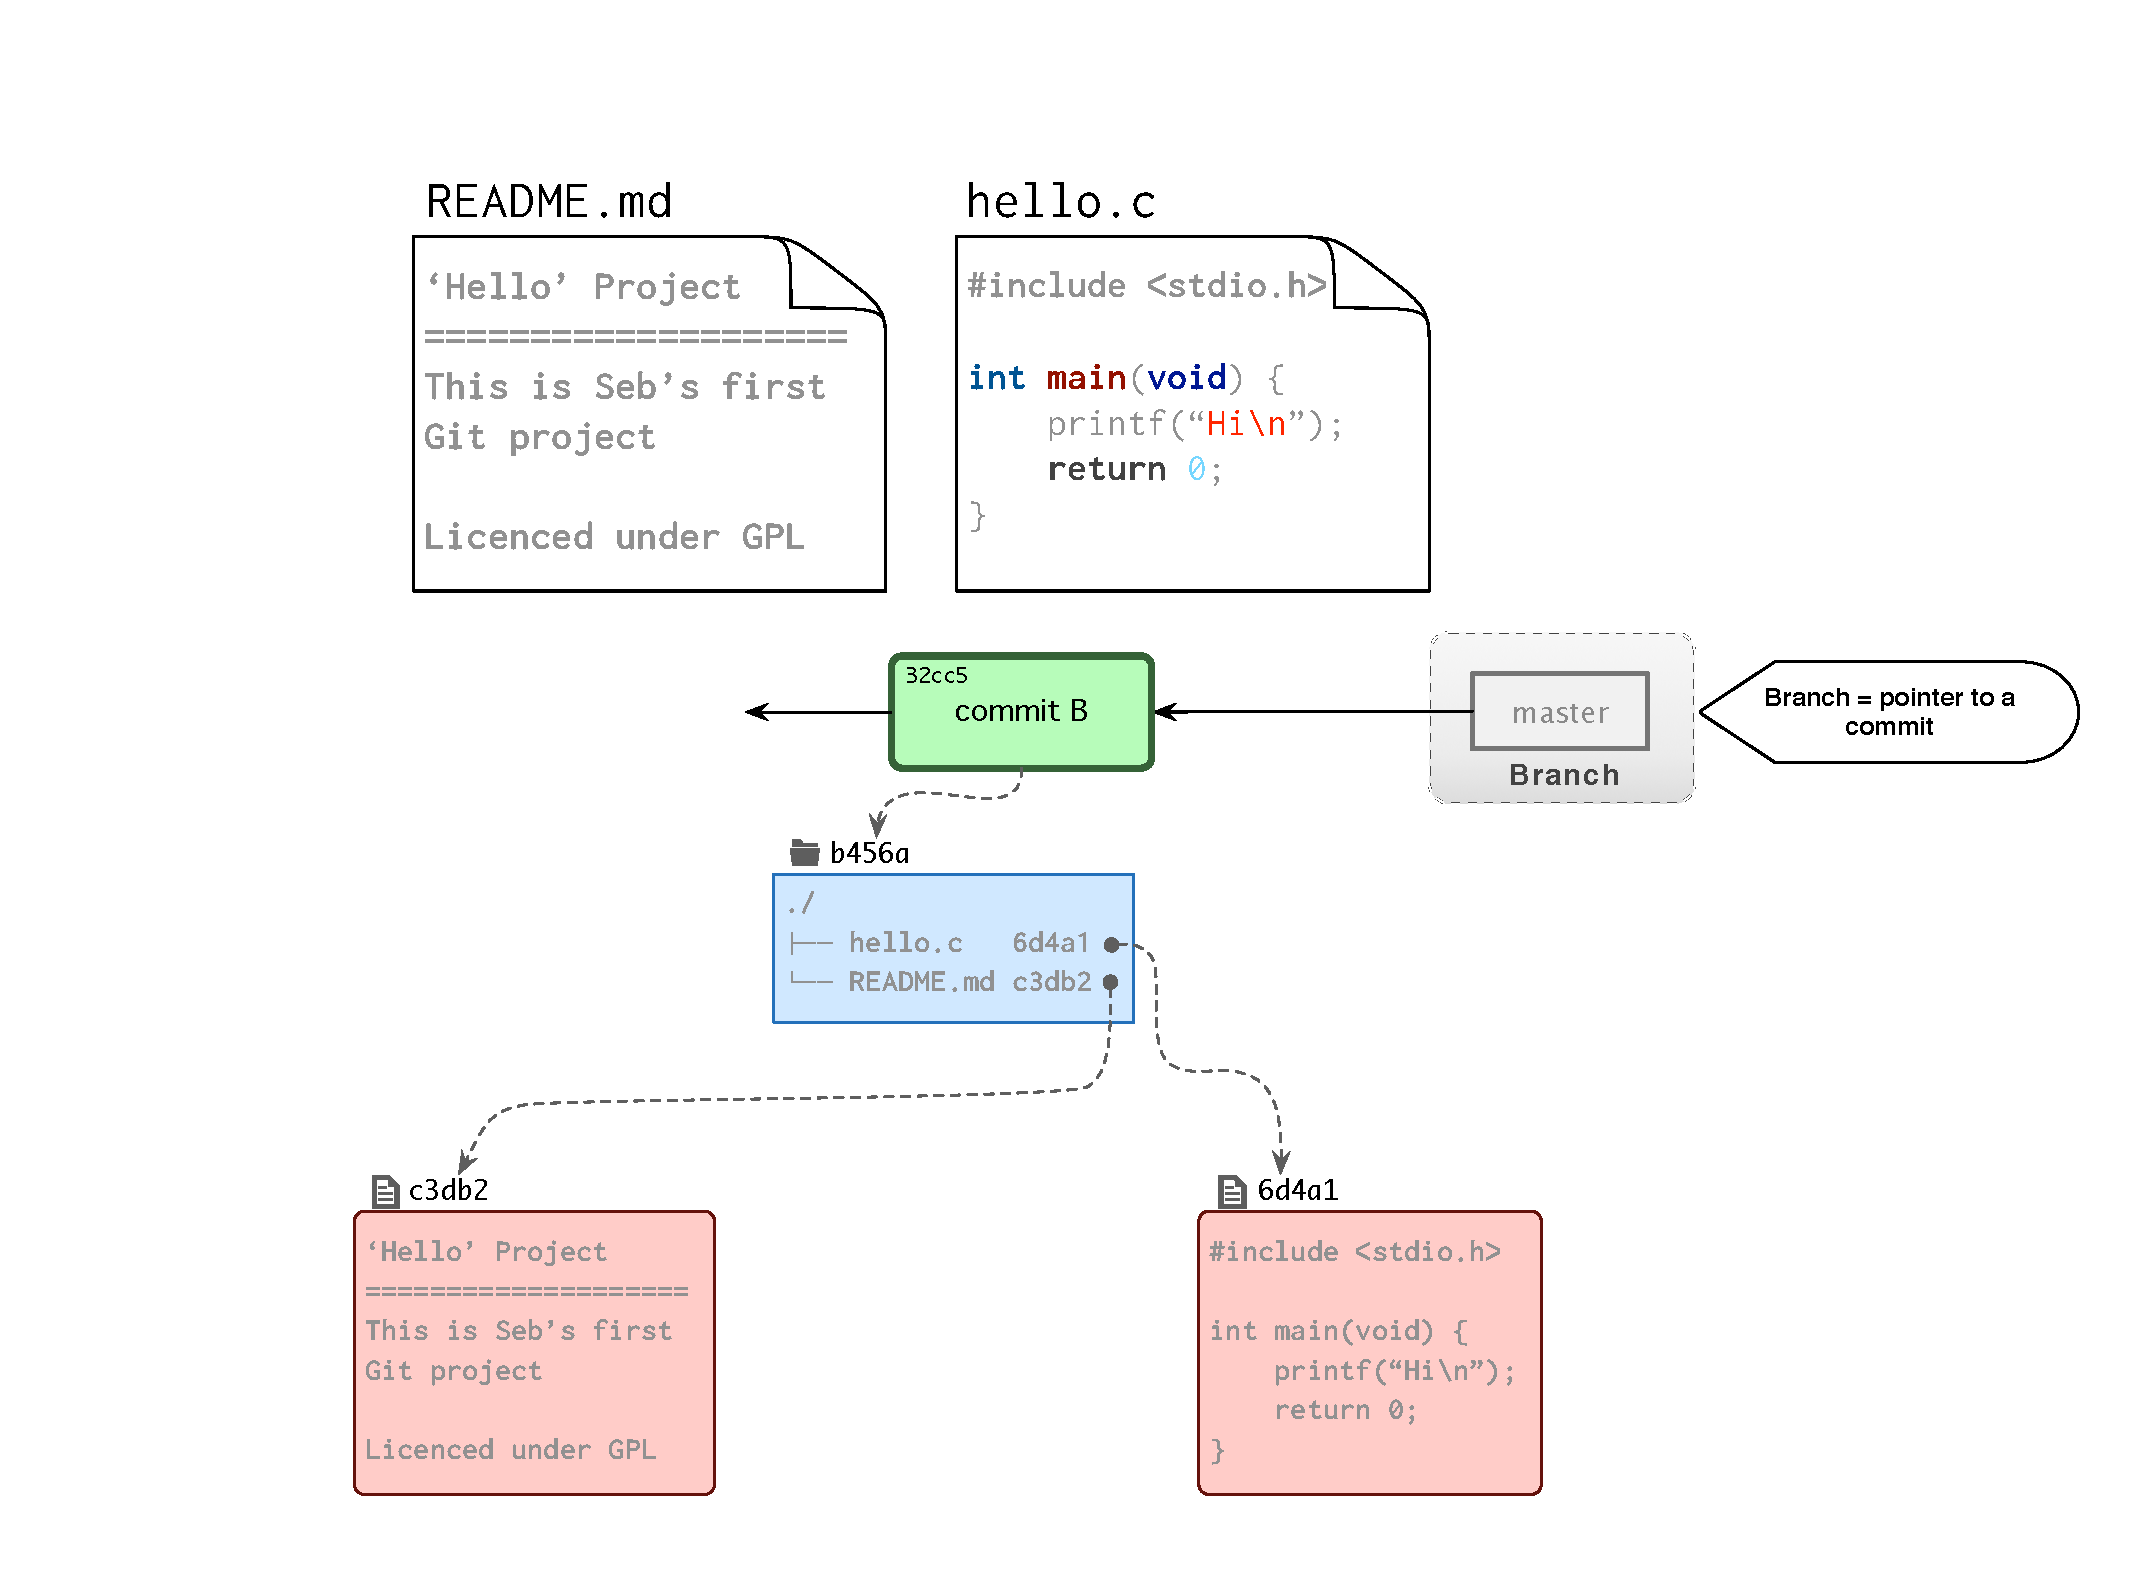
\includegraphics[height=0.95\textheight]{delta_vs_snapshot_example-118.pdf}}
  \only<19>{\includegraphics[height=0.95\textheight]{delta_vs_snapshot_example-119.pdf}}
  \only<20>{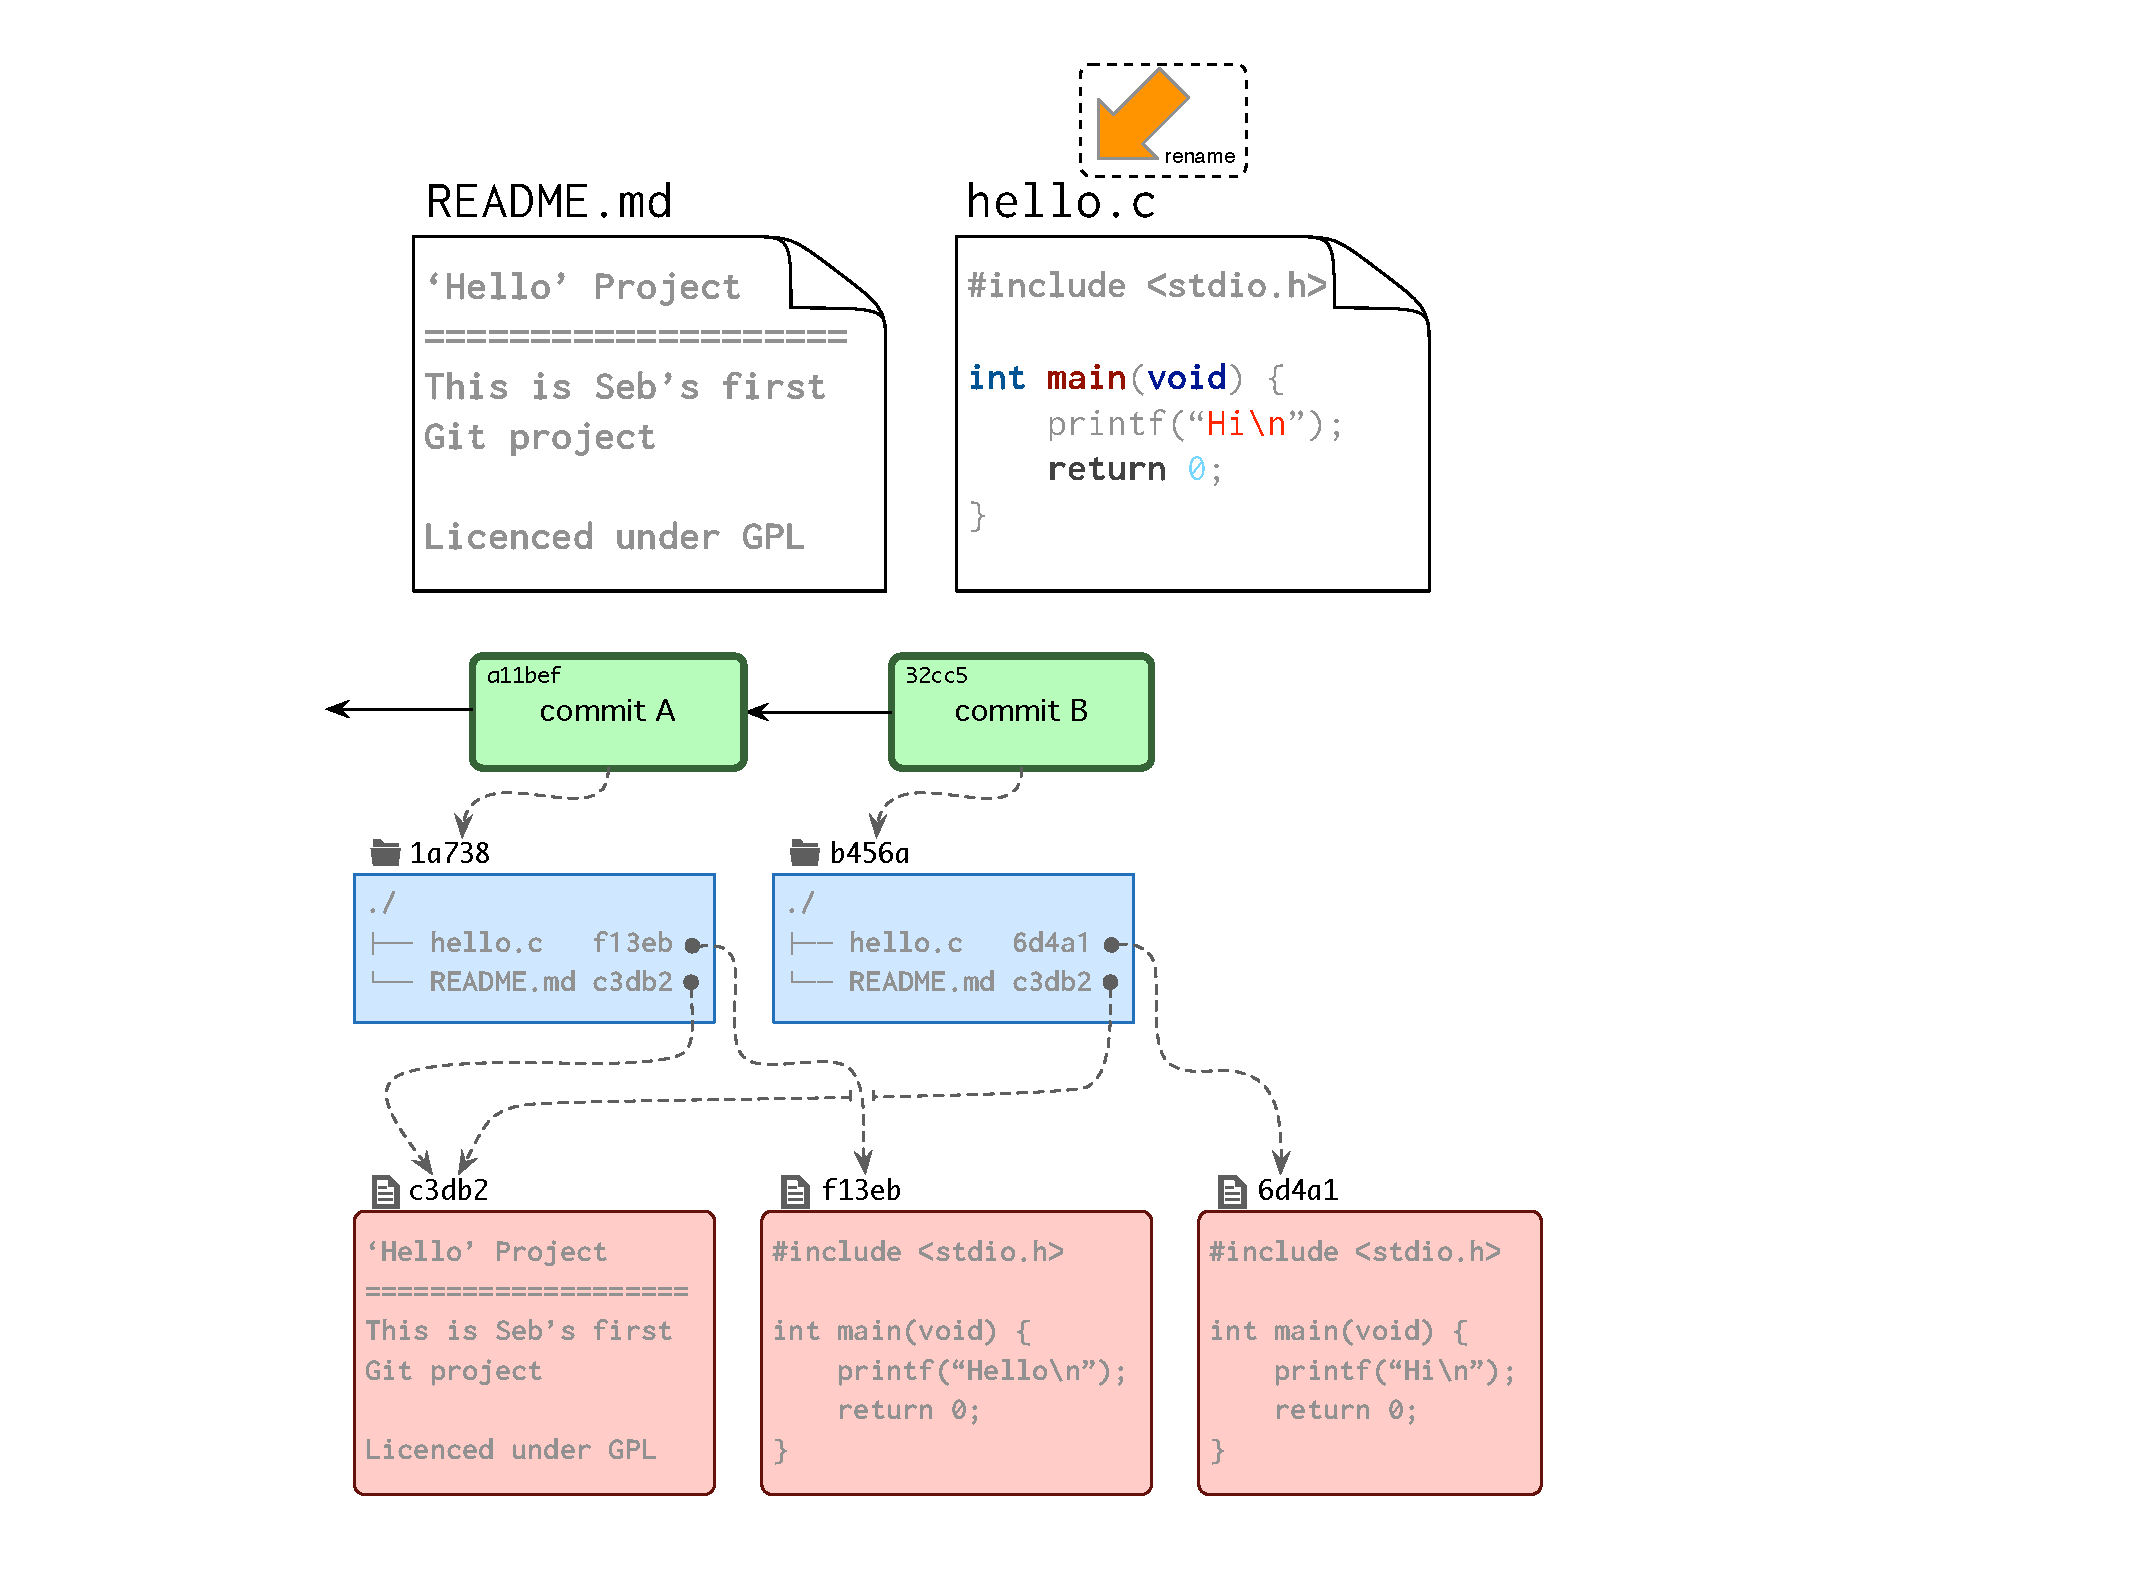
\includegraphics[height=0.95\textheight]{delta_vs_snapshot_example-120.pdf}}
  \only<21>{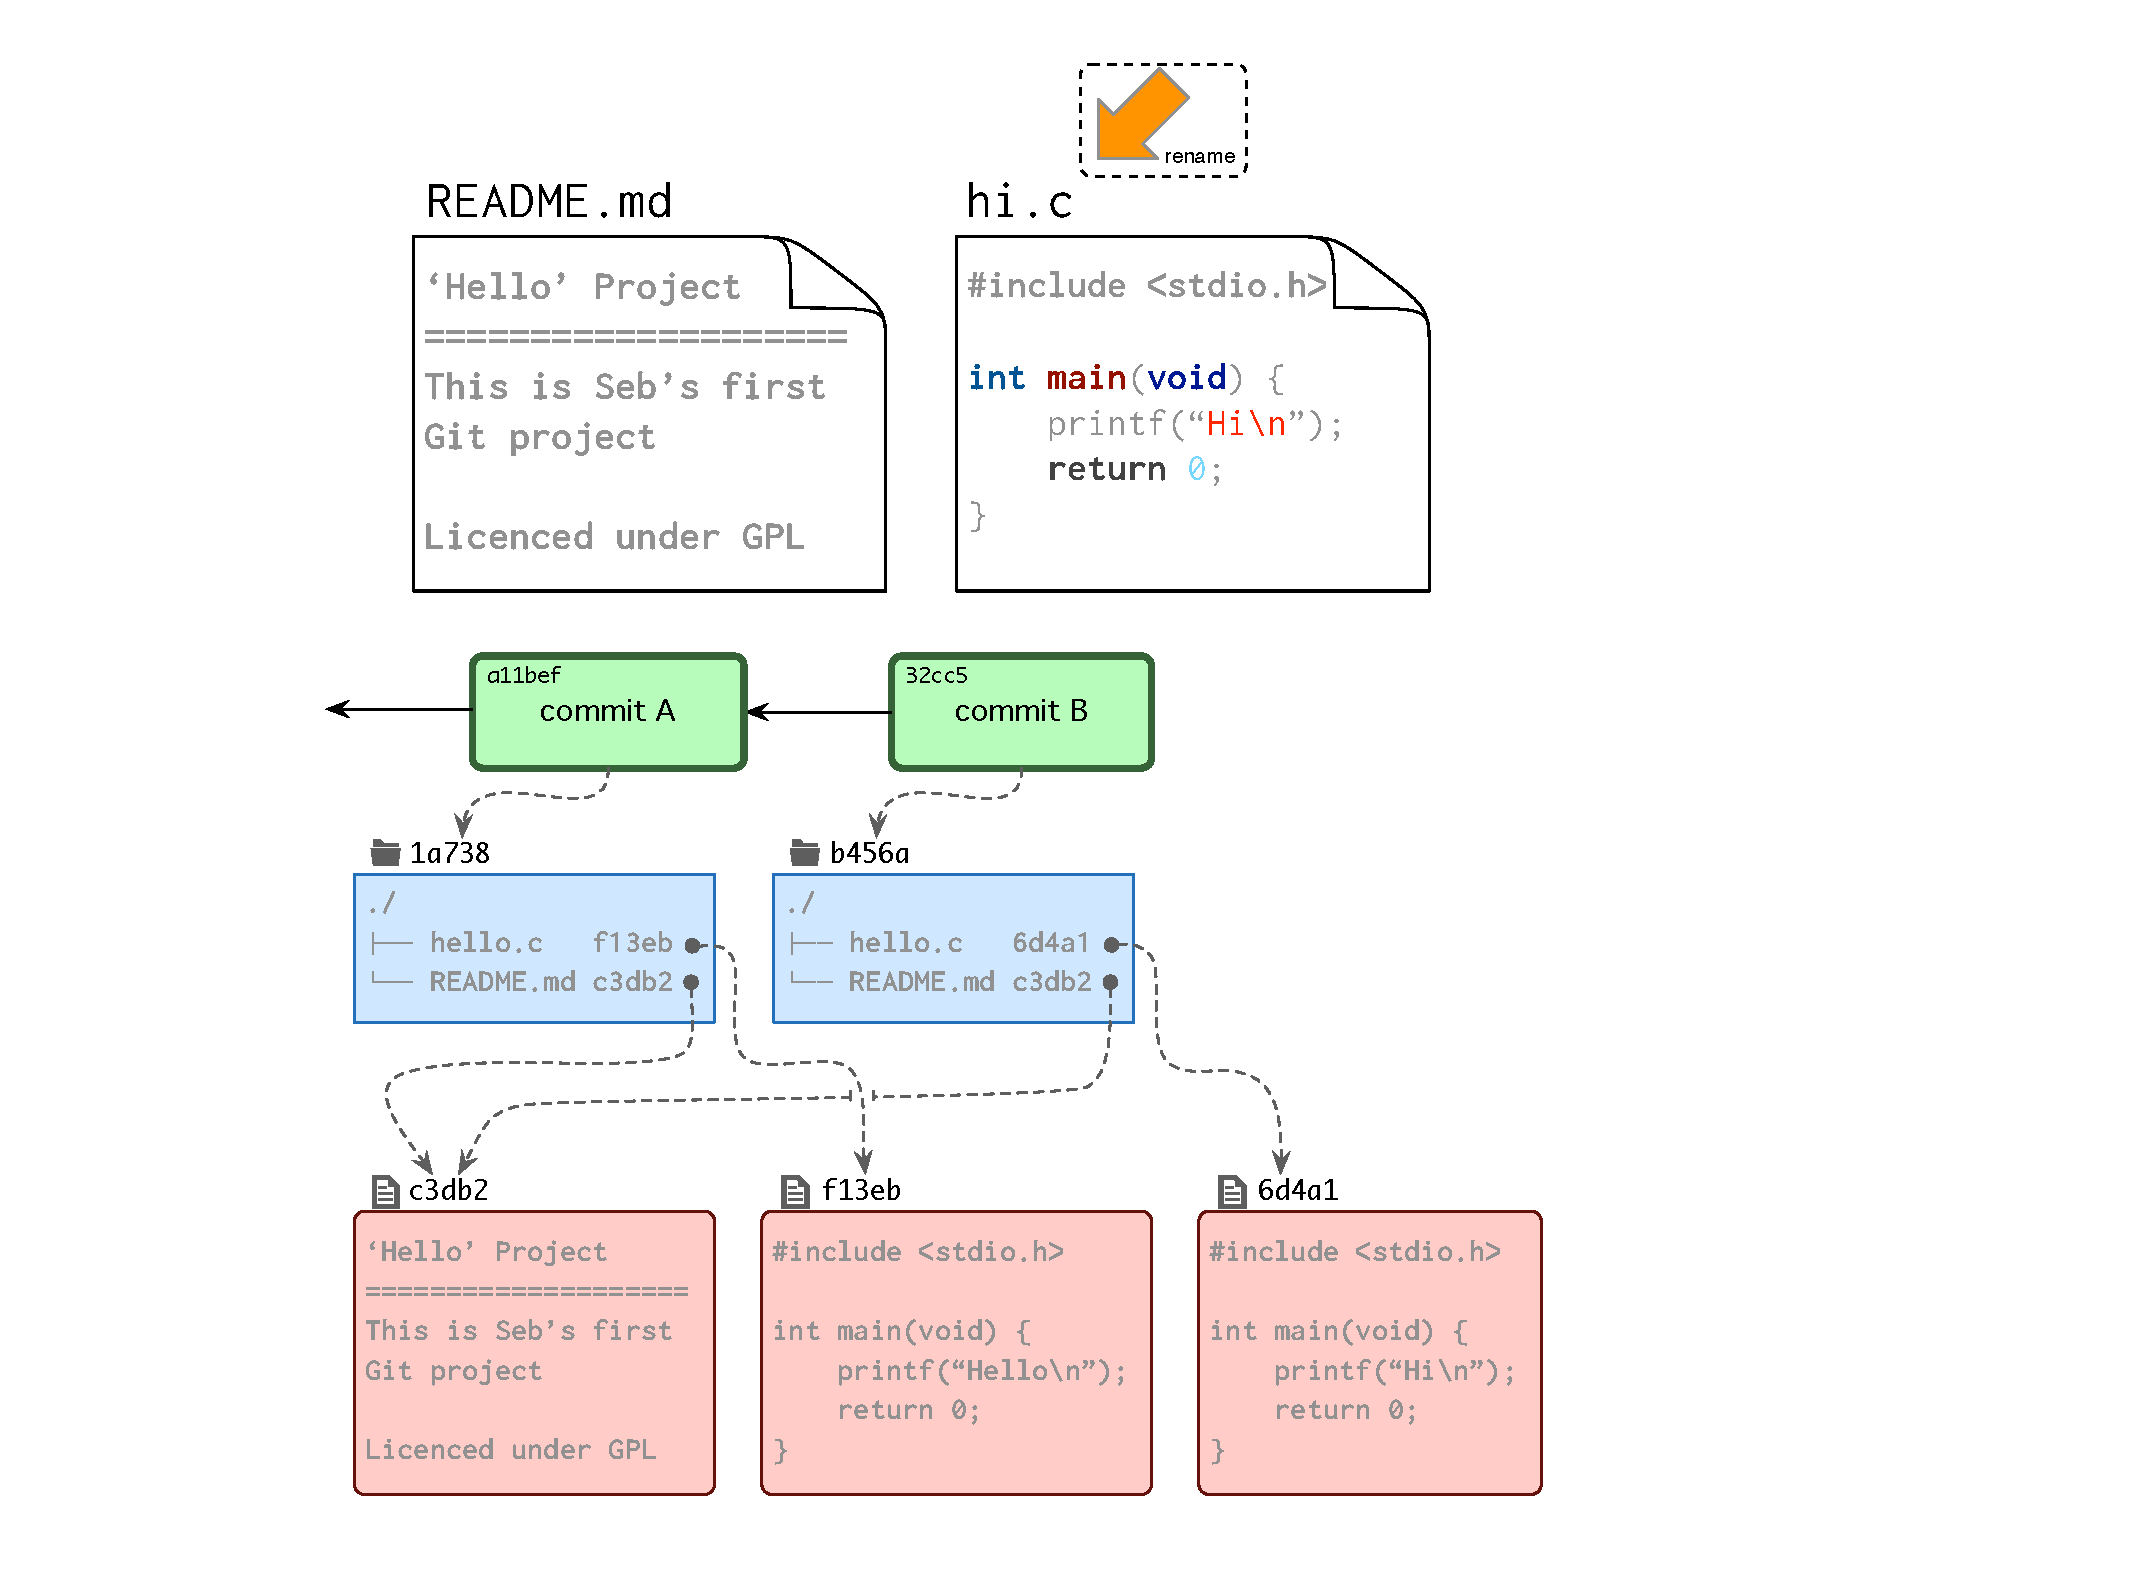
\includegraphics[height=0.95\textheight]{delta_vs_snapshot_example-121.pdf}}
  \only<22>{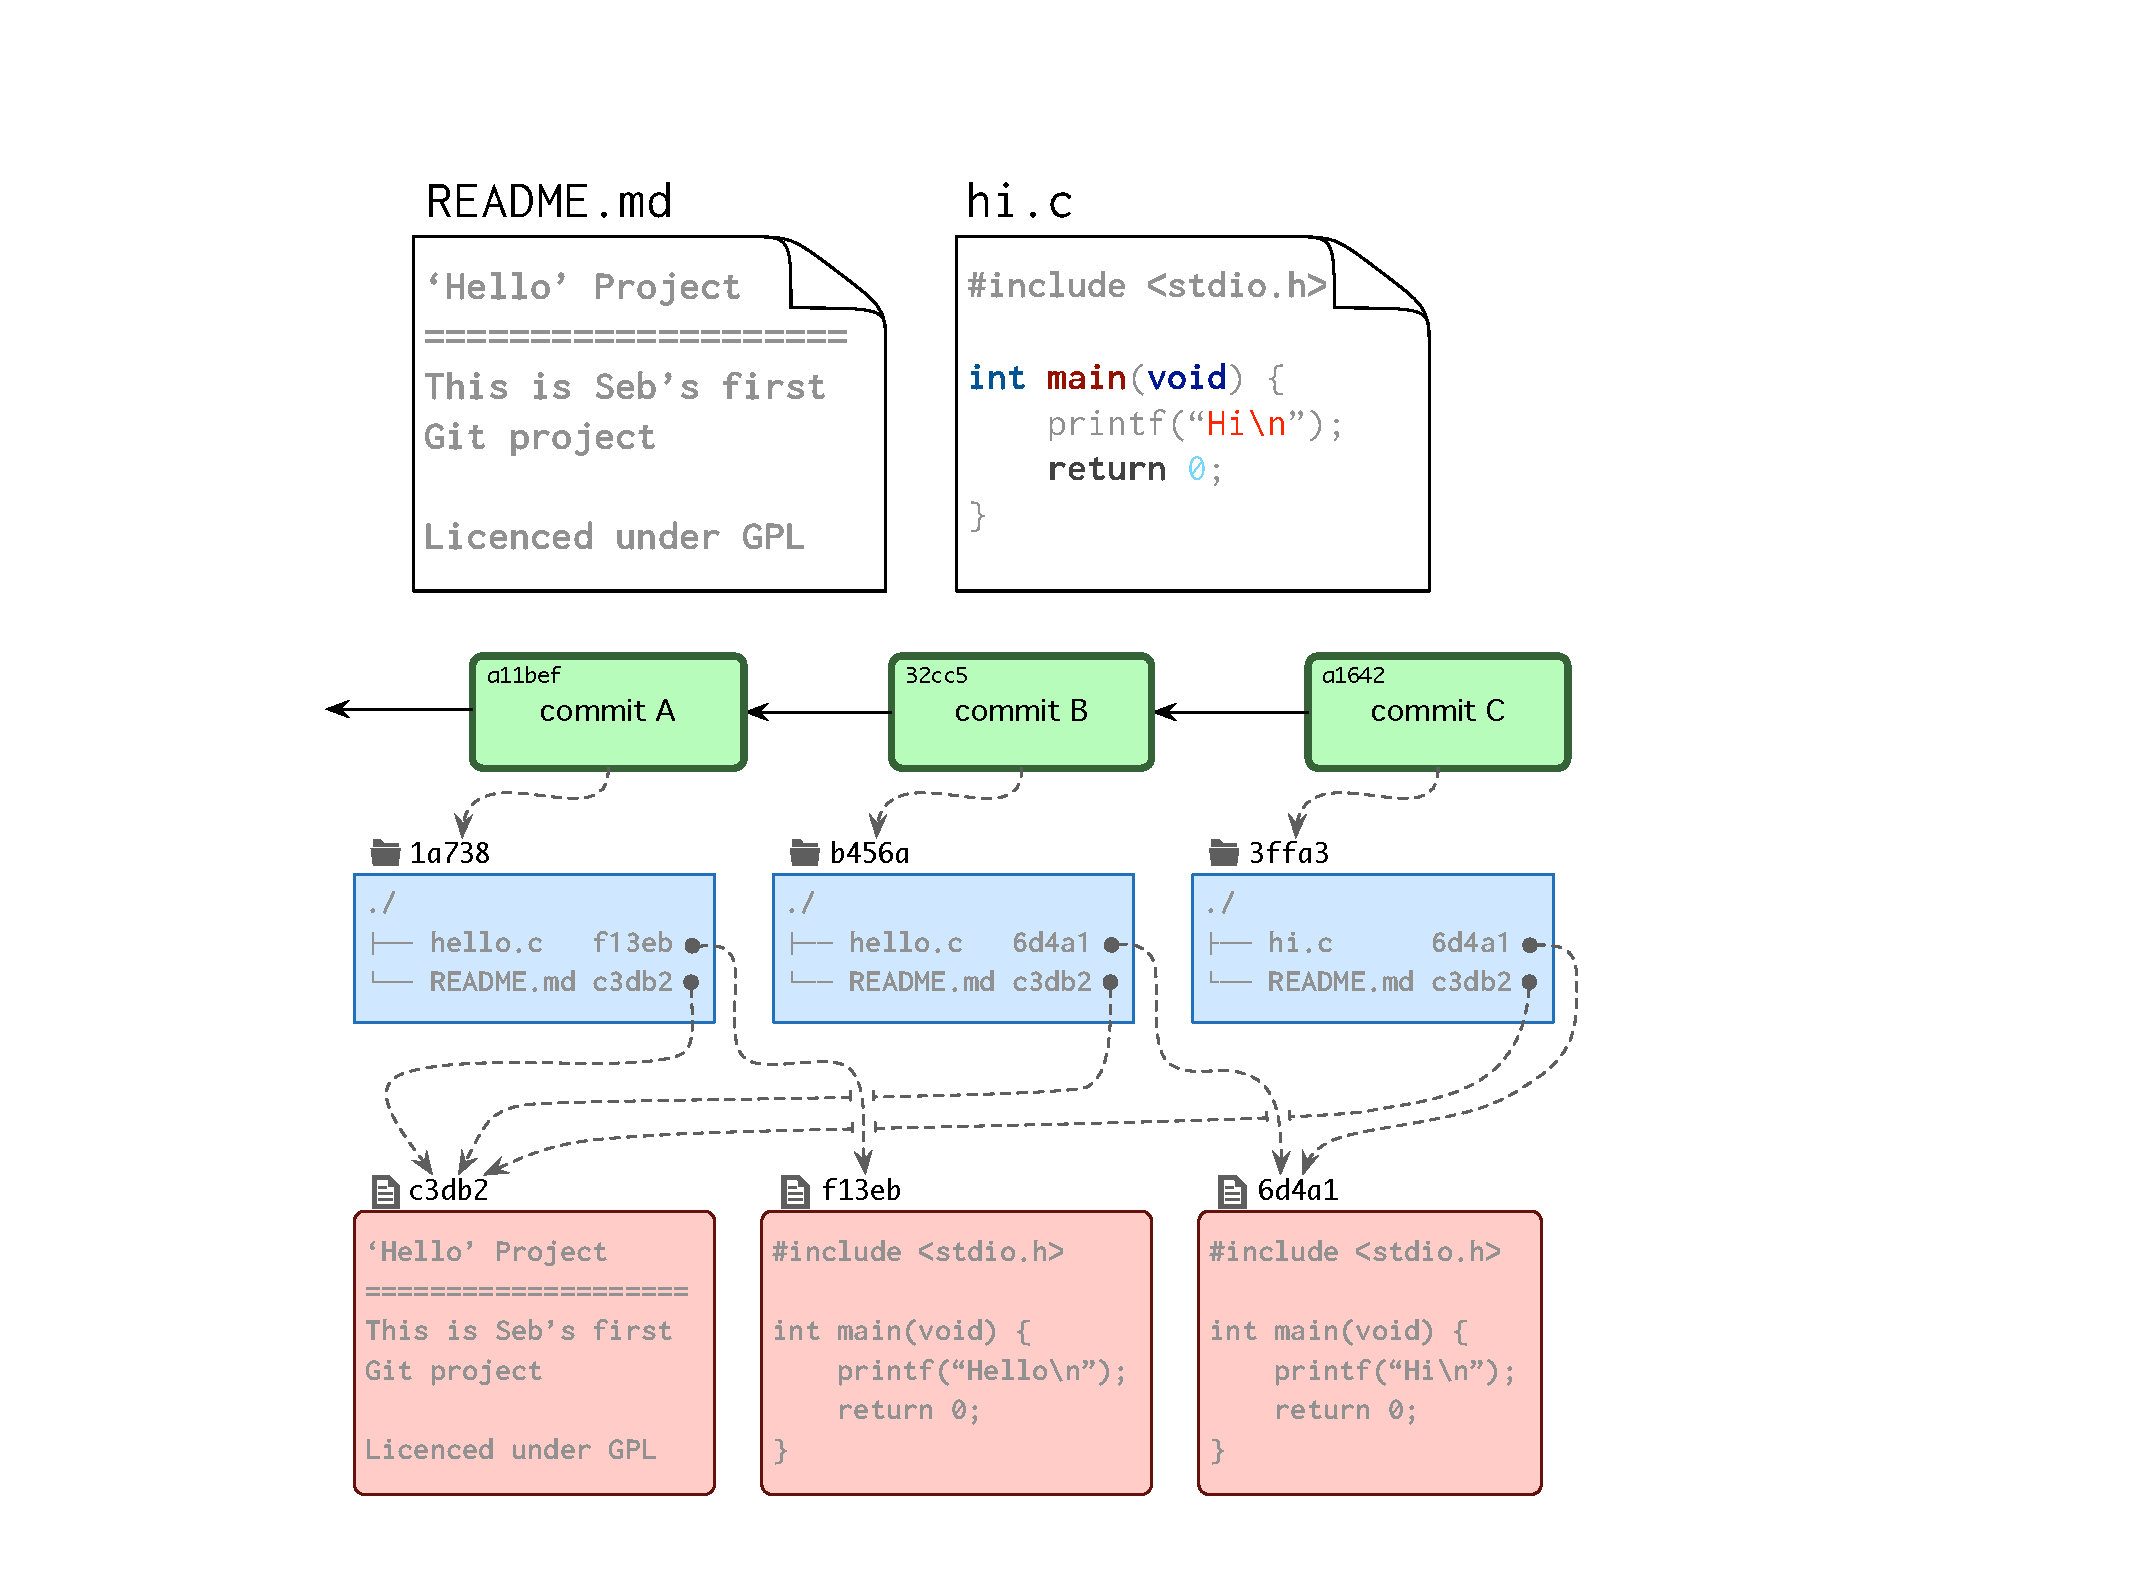
\includegraphics[height=0.95\textheight]{delta_vs_snapshot_example-122.pdf}}
  \only<23>{\includegraphics[height=0.95\textheight]{delta_vs_snapshot_example-123.pdf}}
  \only<24>{\includegraphics[height=0.95\textheight]{delta_vs_snapshot_example-124.pdf}}
  \only<25>{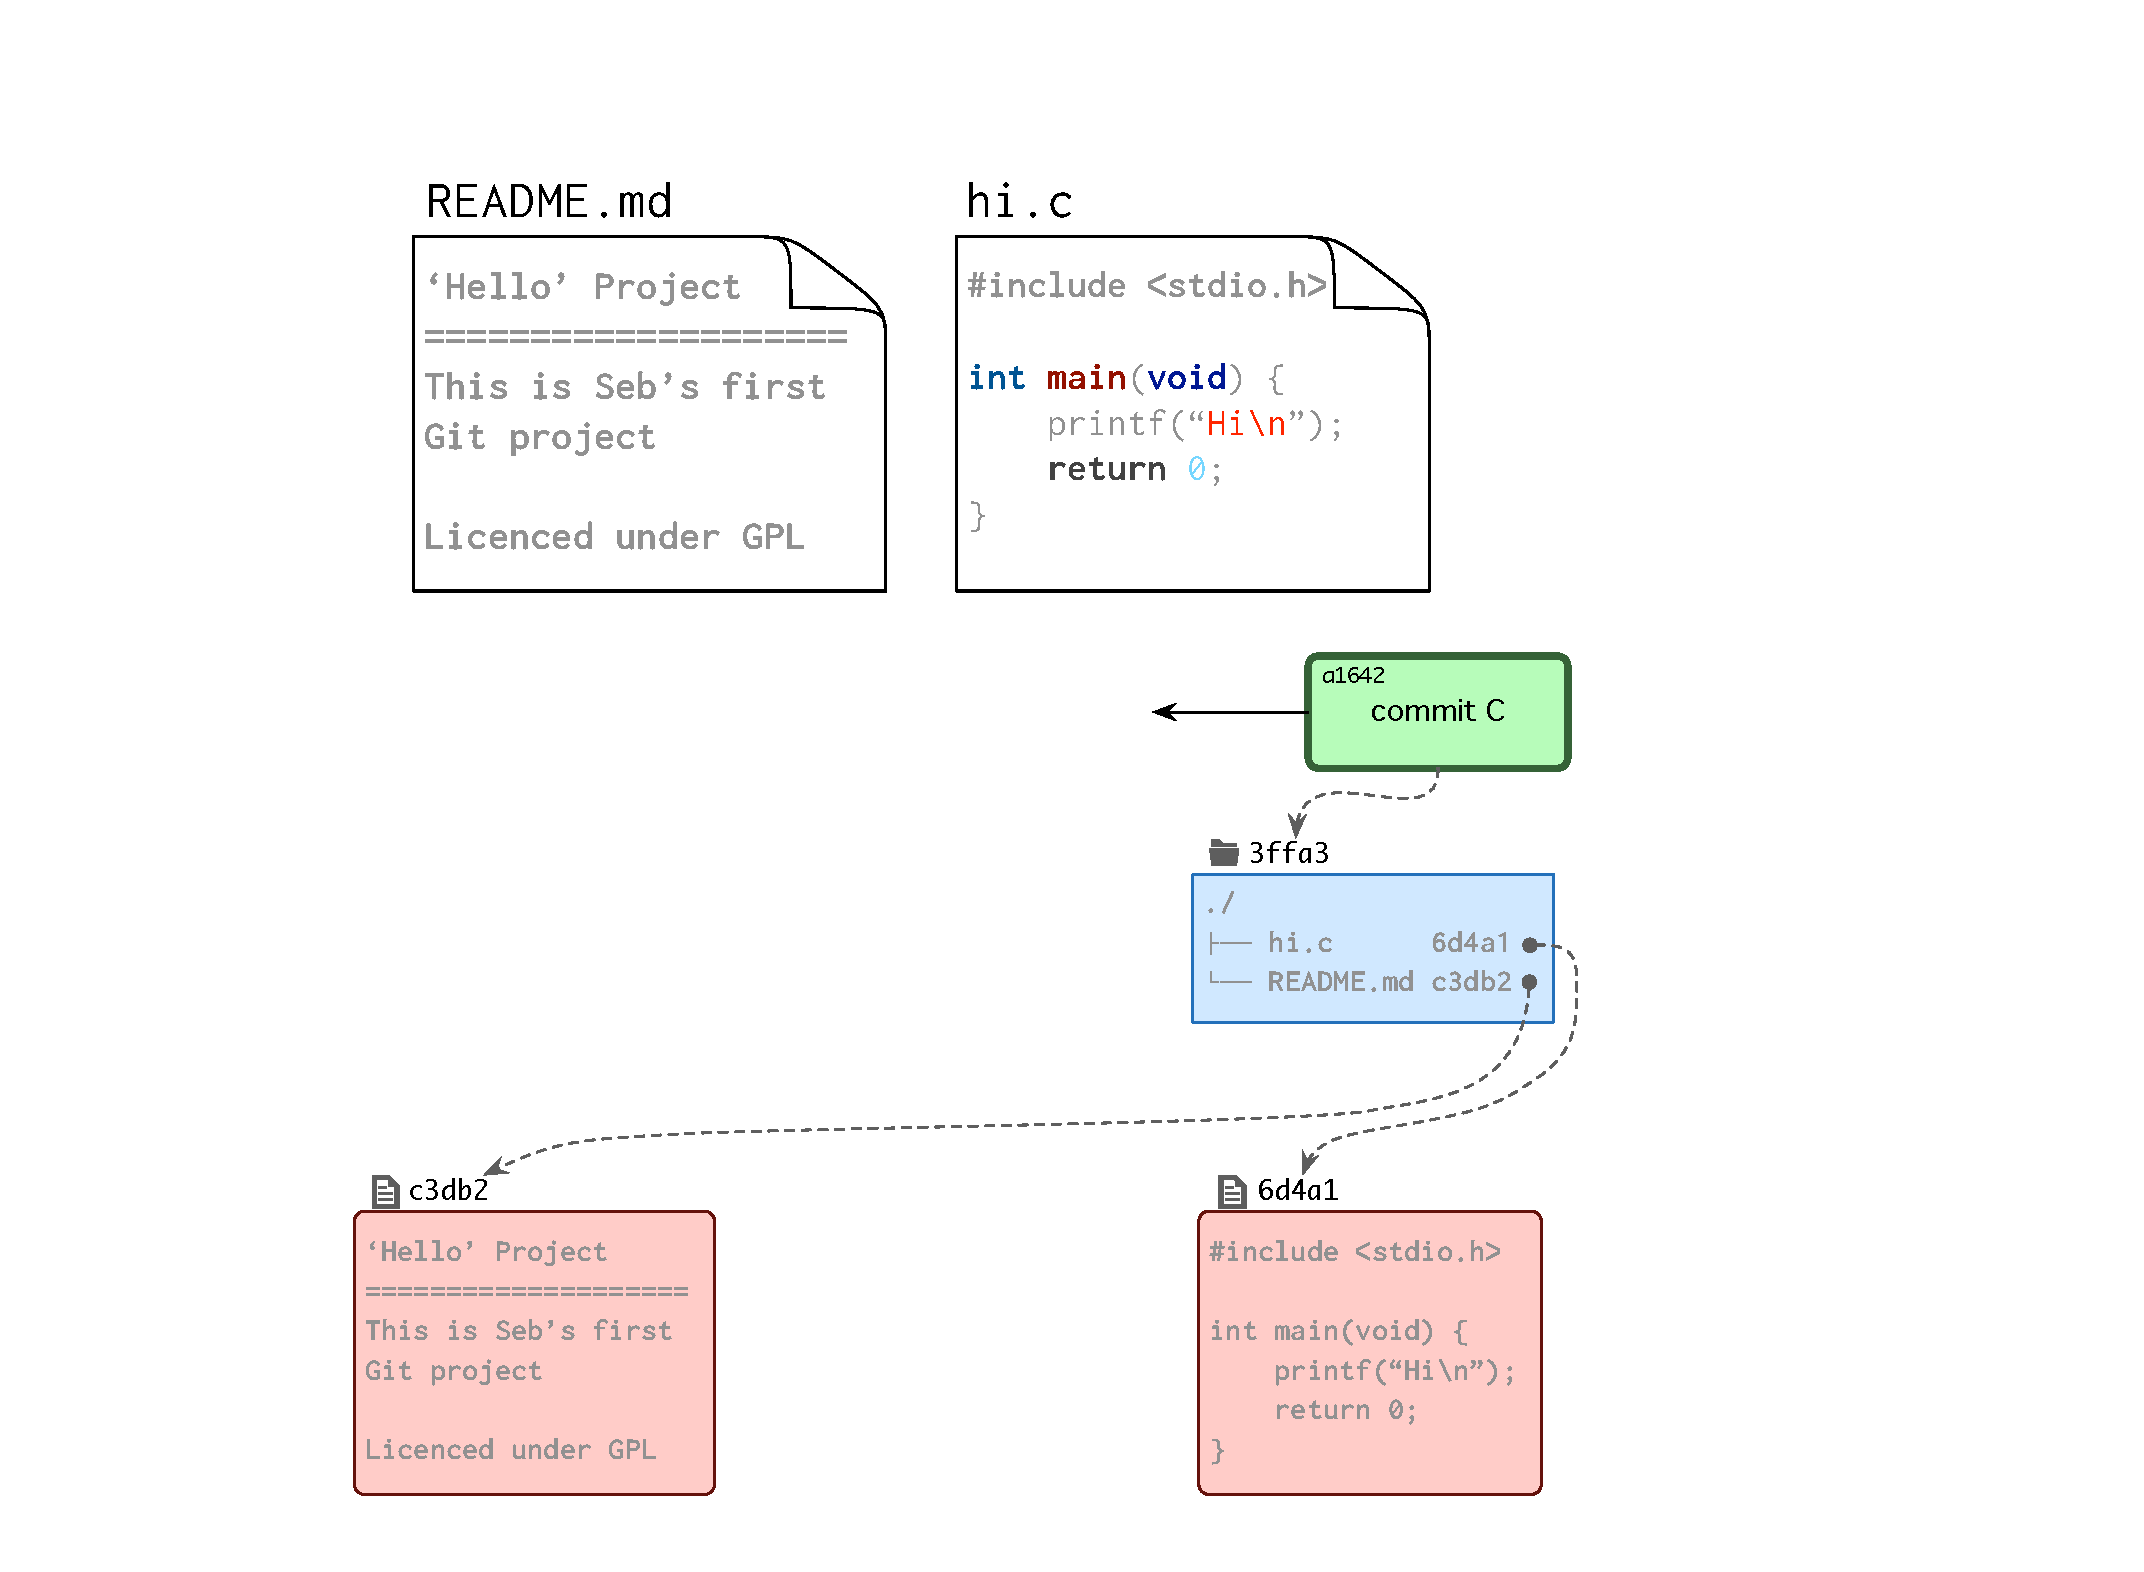
\includegraphics[height=0.95\textheight]{delta_vs_snapshot_example-125.pdf}}
  \only<26>{\includegraphics[height=0.95\textheight]{delta_vs_snapshot_example-126.pdf}}
  \only<27>{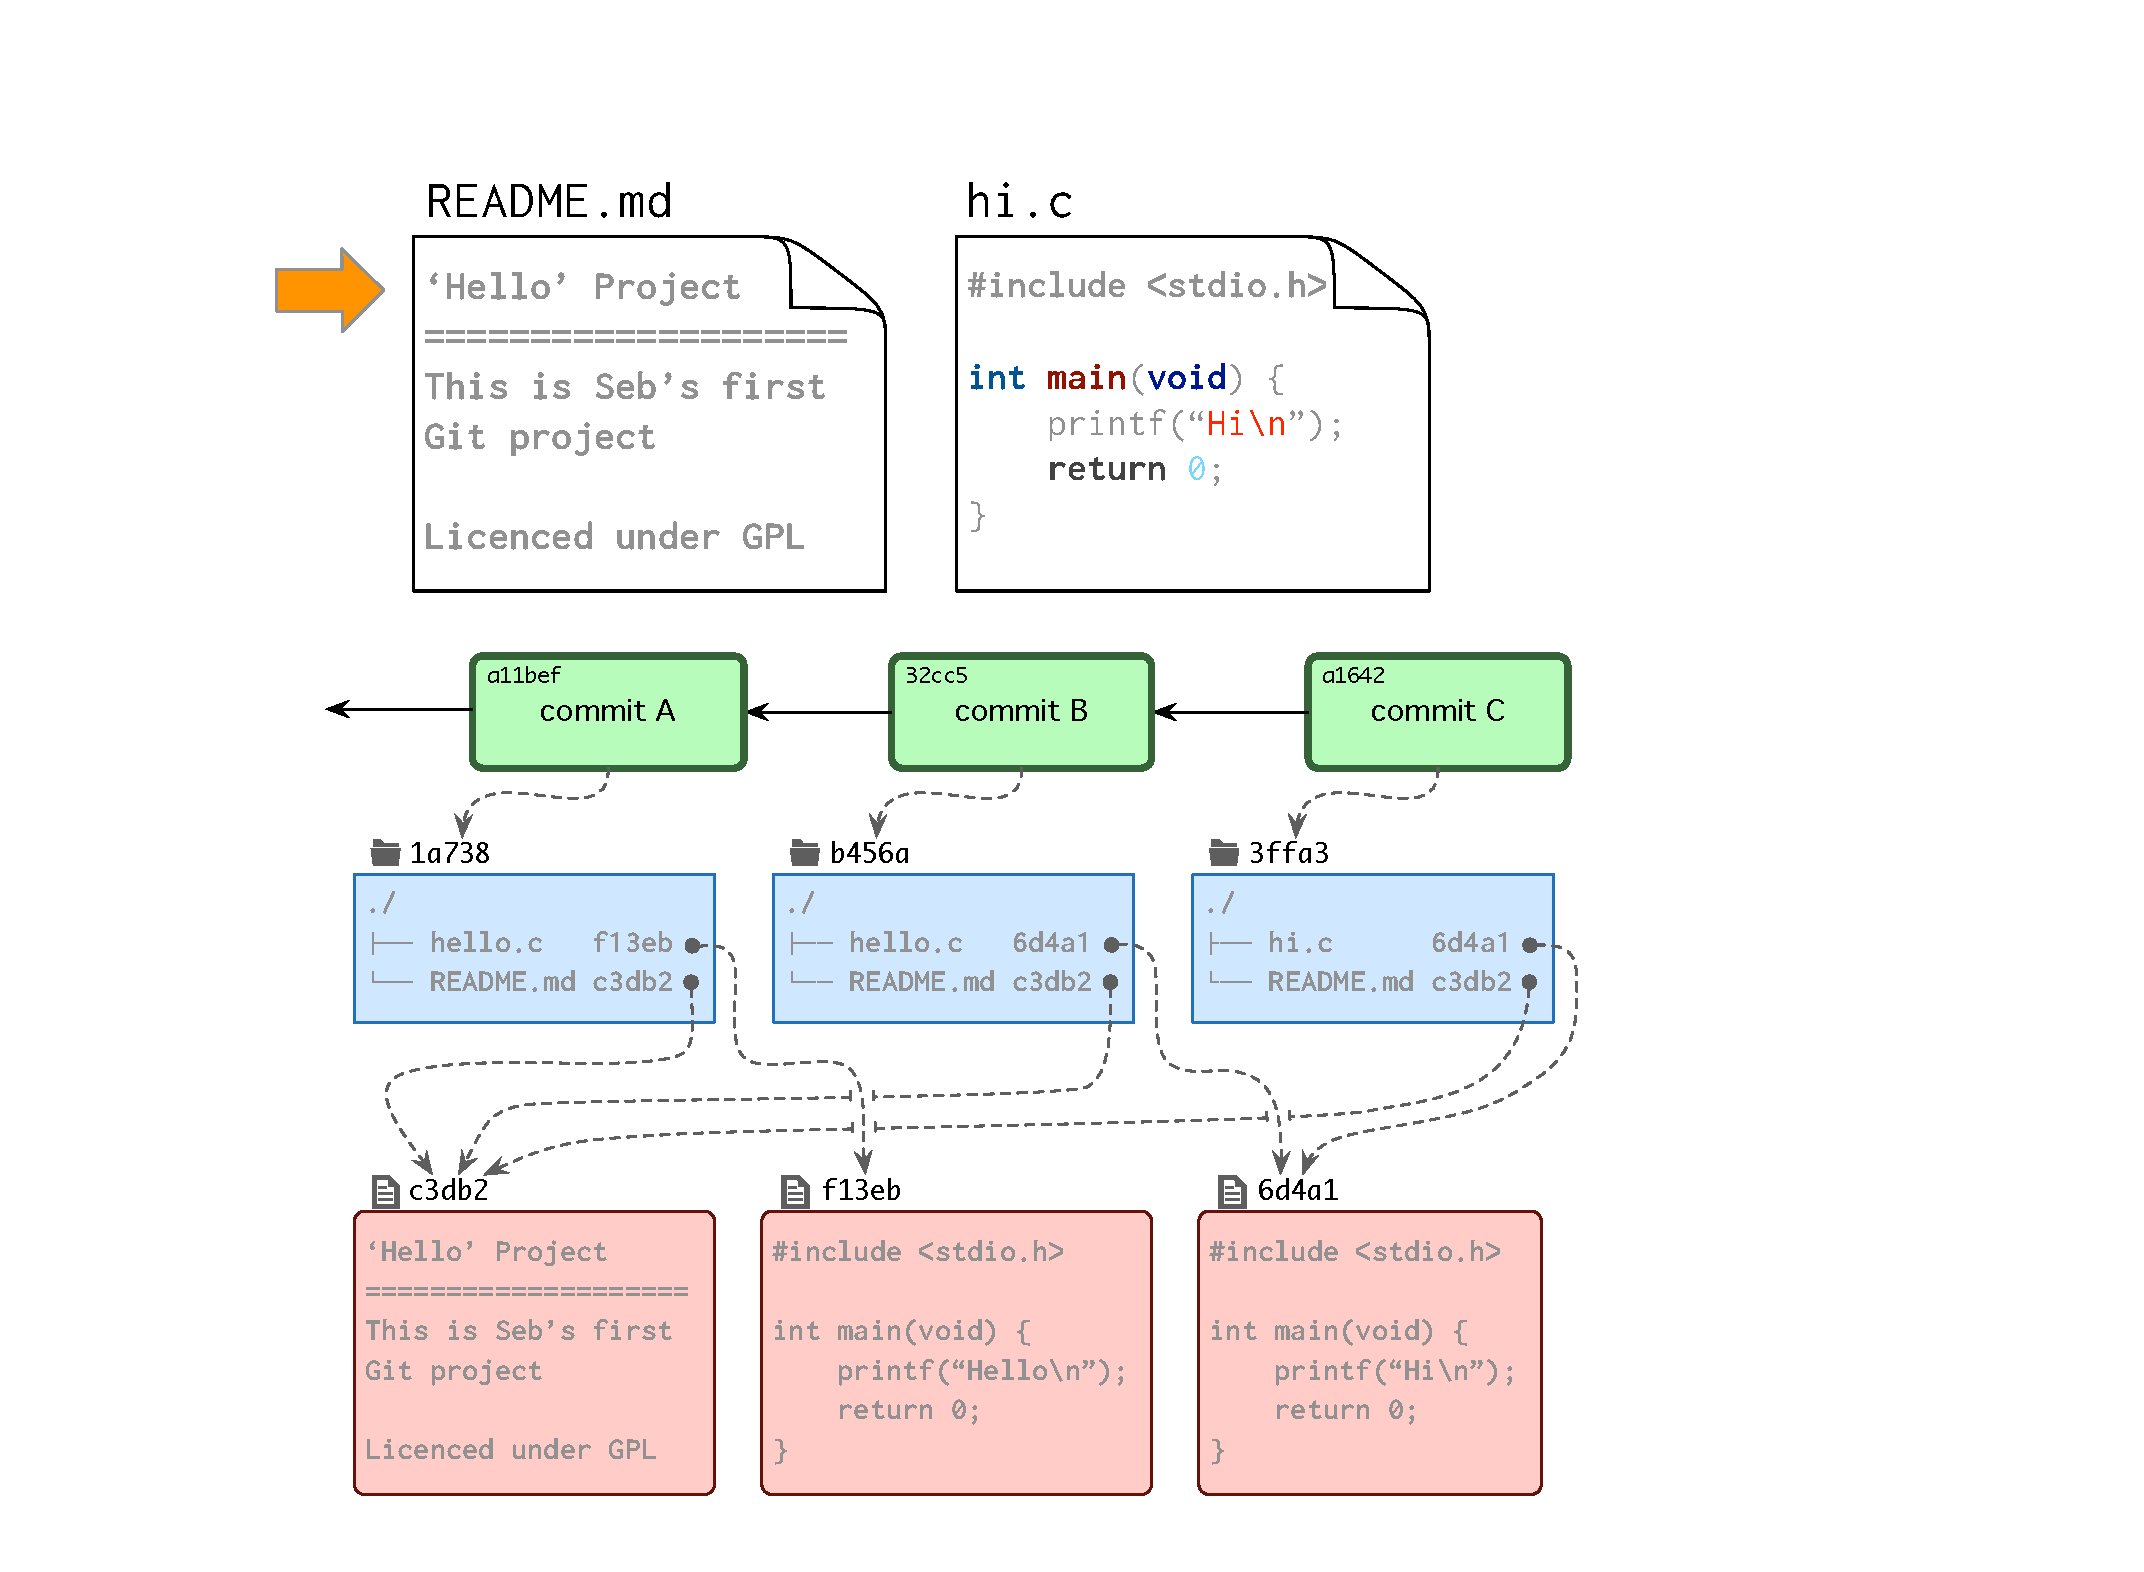
\includegraphics[height=0.95\textheight]{delta_vs_snapshot_example-127.pdf}}
  \only<28>{\includegraphics[height=0.95\textheight]{delta_vs_snapshot_example-128.pdf}}
  \only<29>{\includegraphics[height=0.95\textheight]{delta_vs_snapshot_example-129.pdf}}
  \only<30>{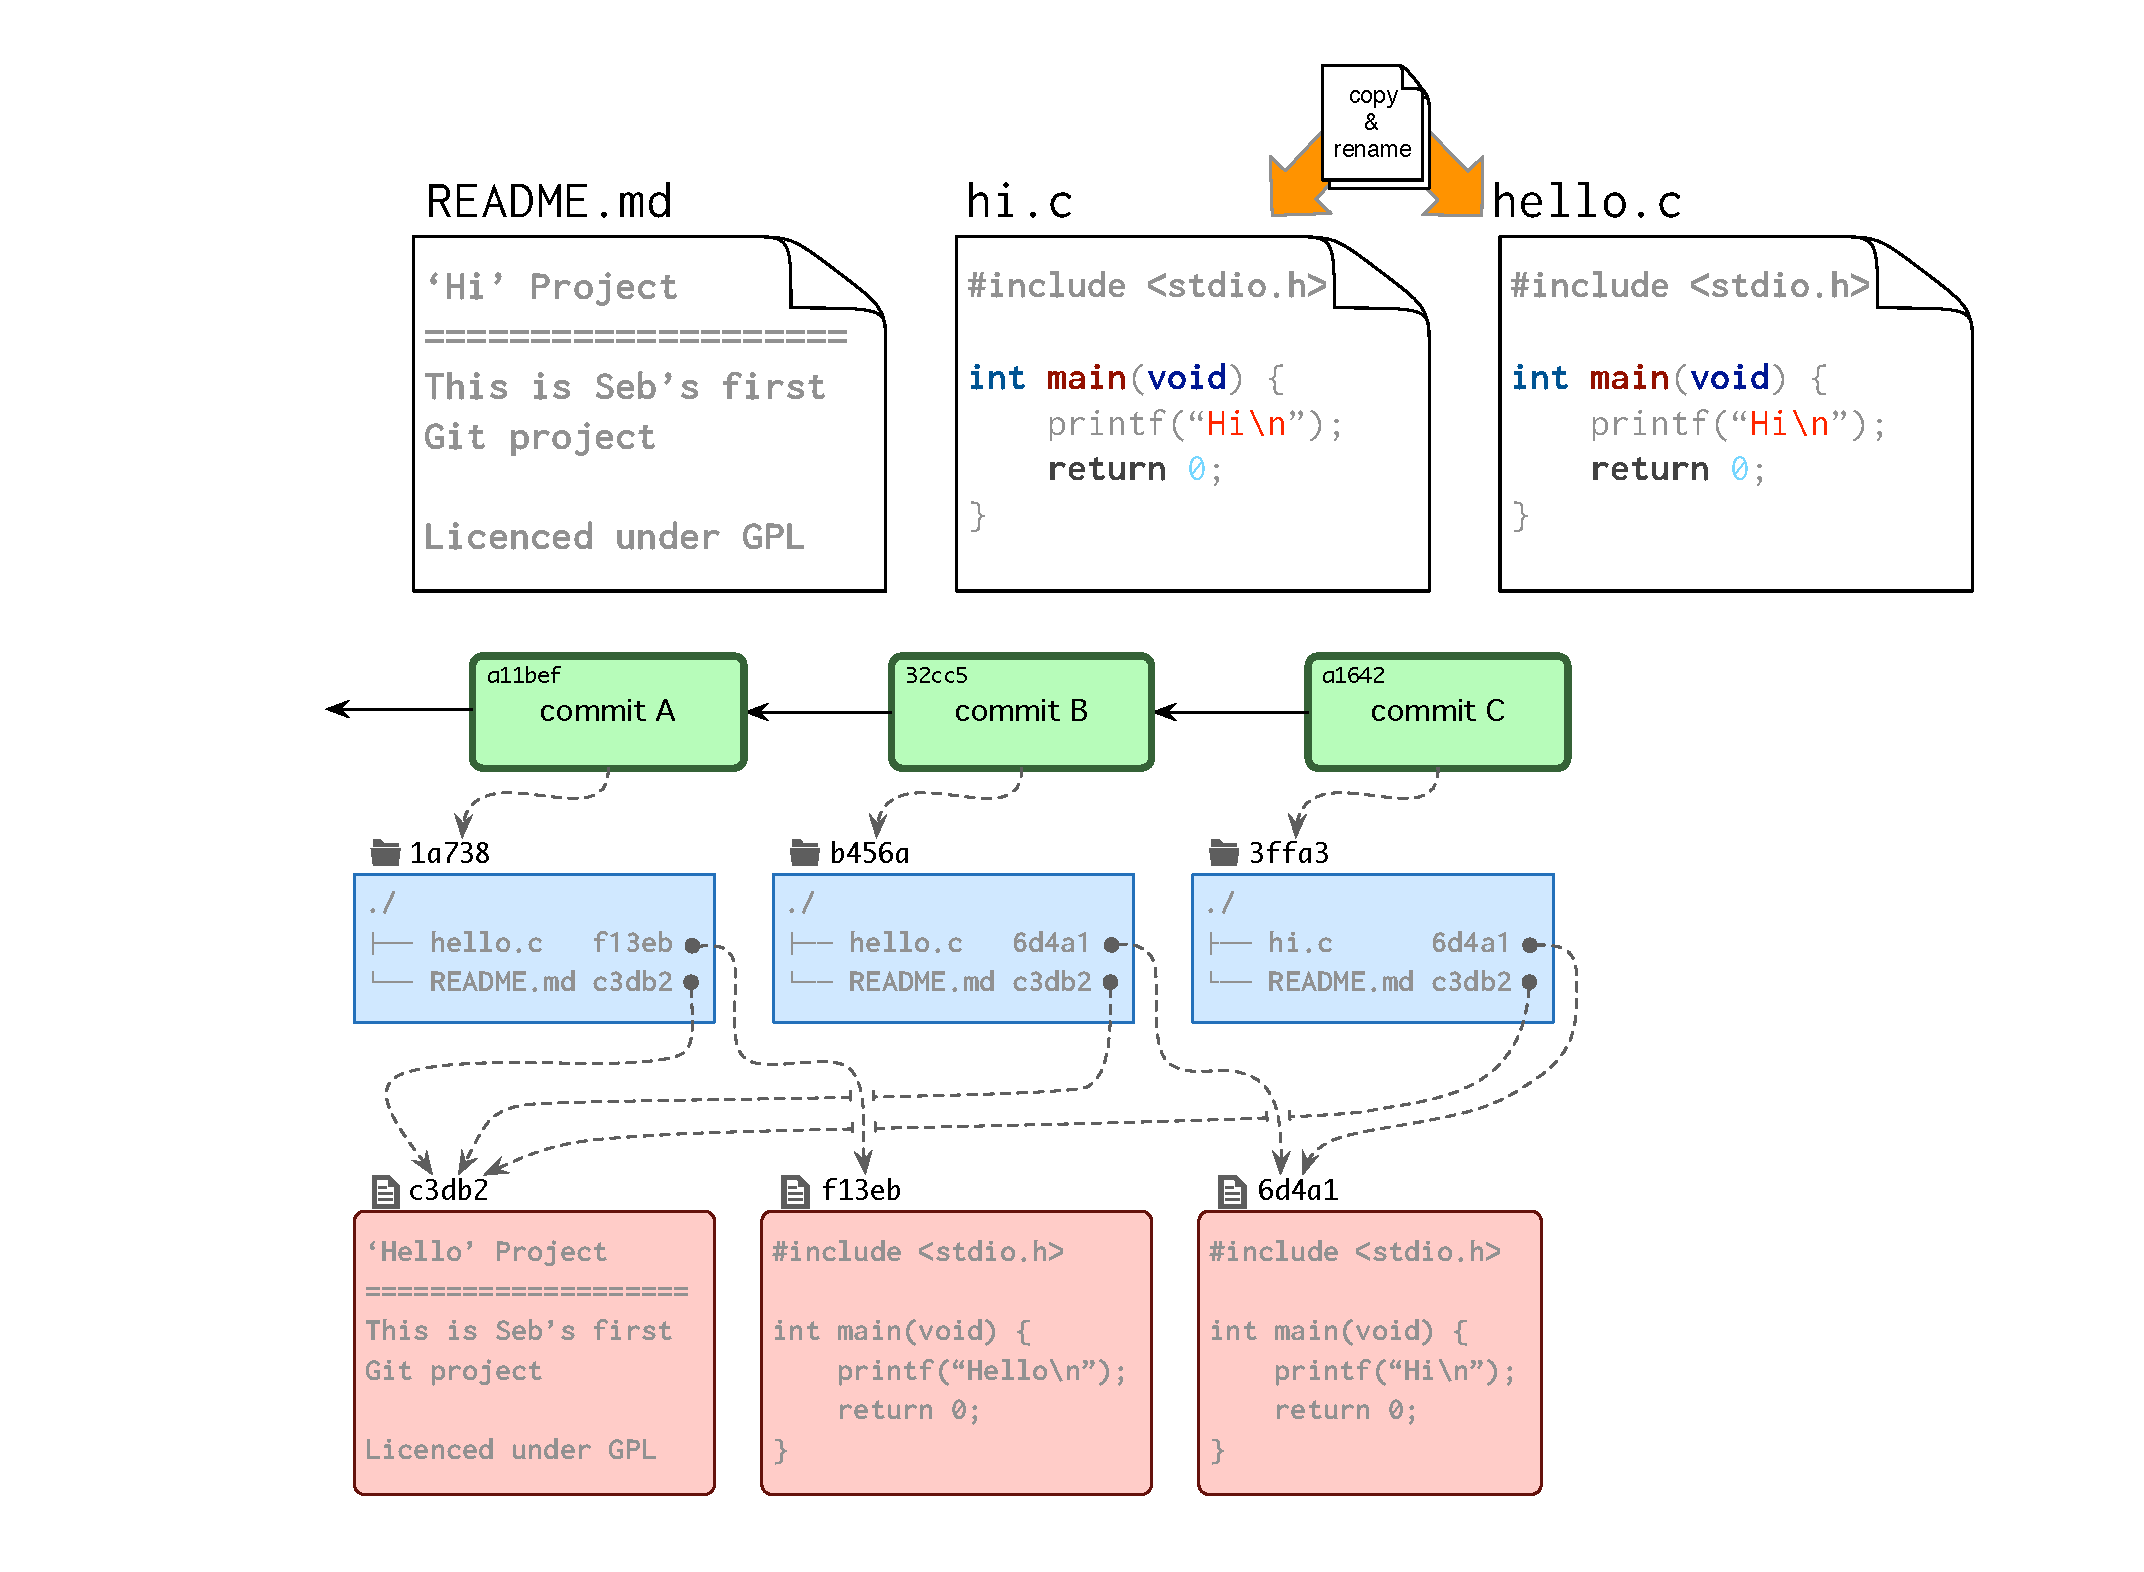
\includegraphics[height=0.95\textheight]{delta_vs_snapshot_example-130.pdf}}
  \only<31>{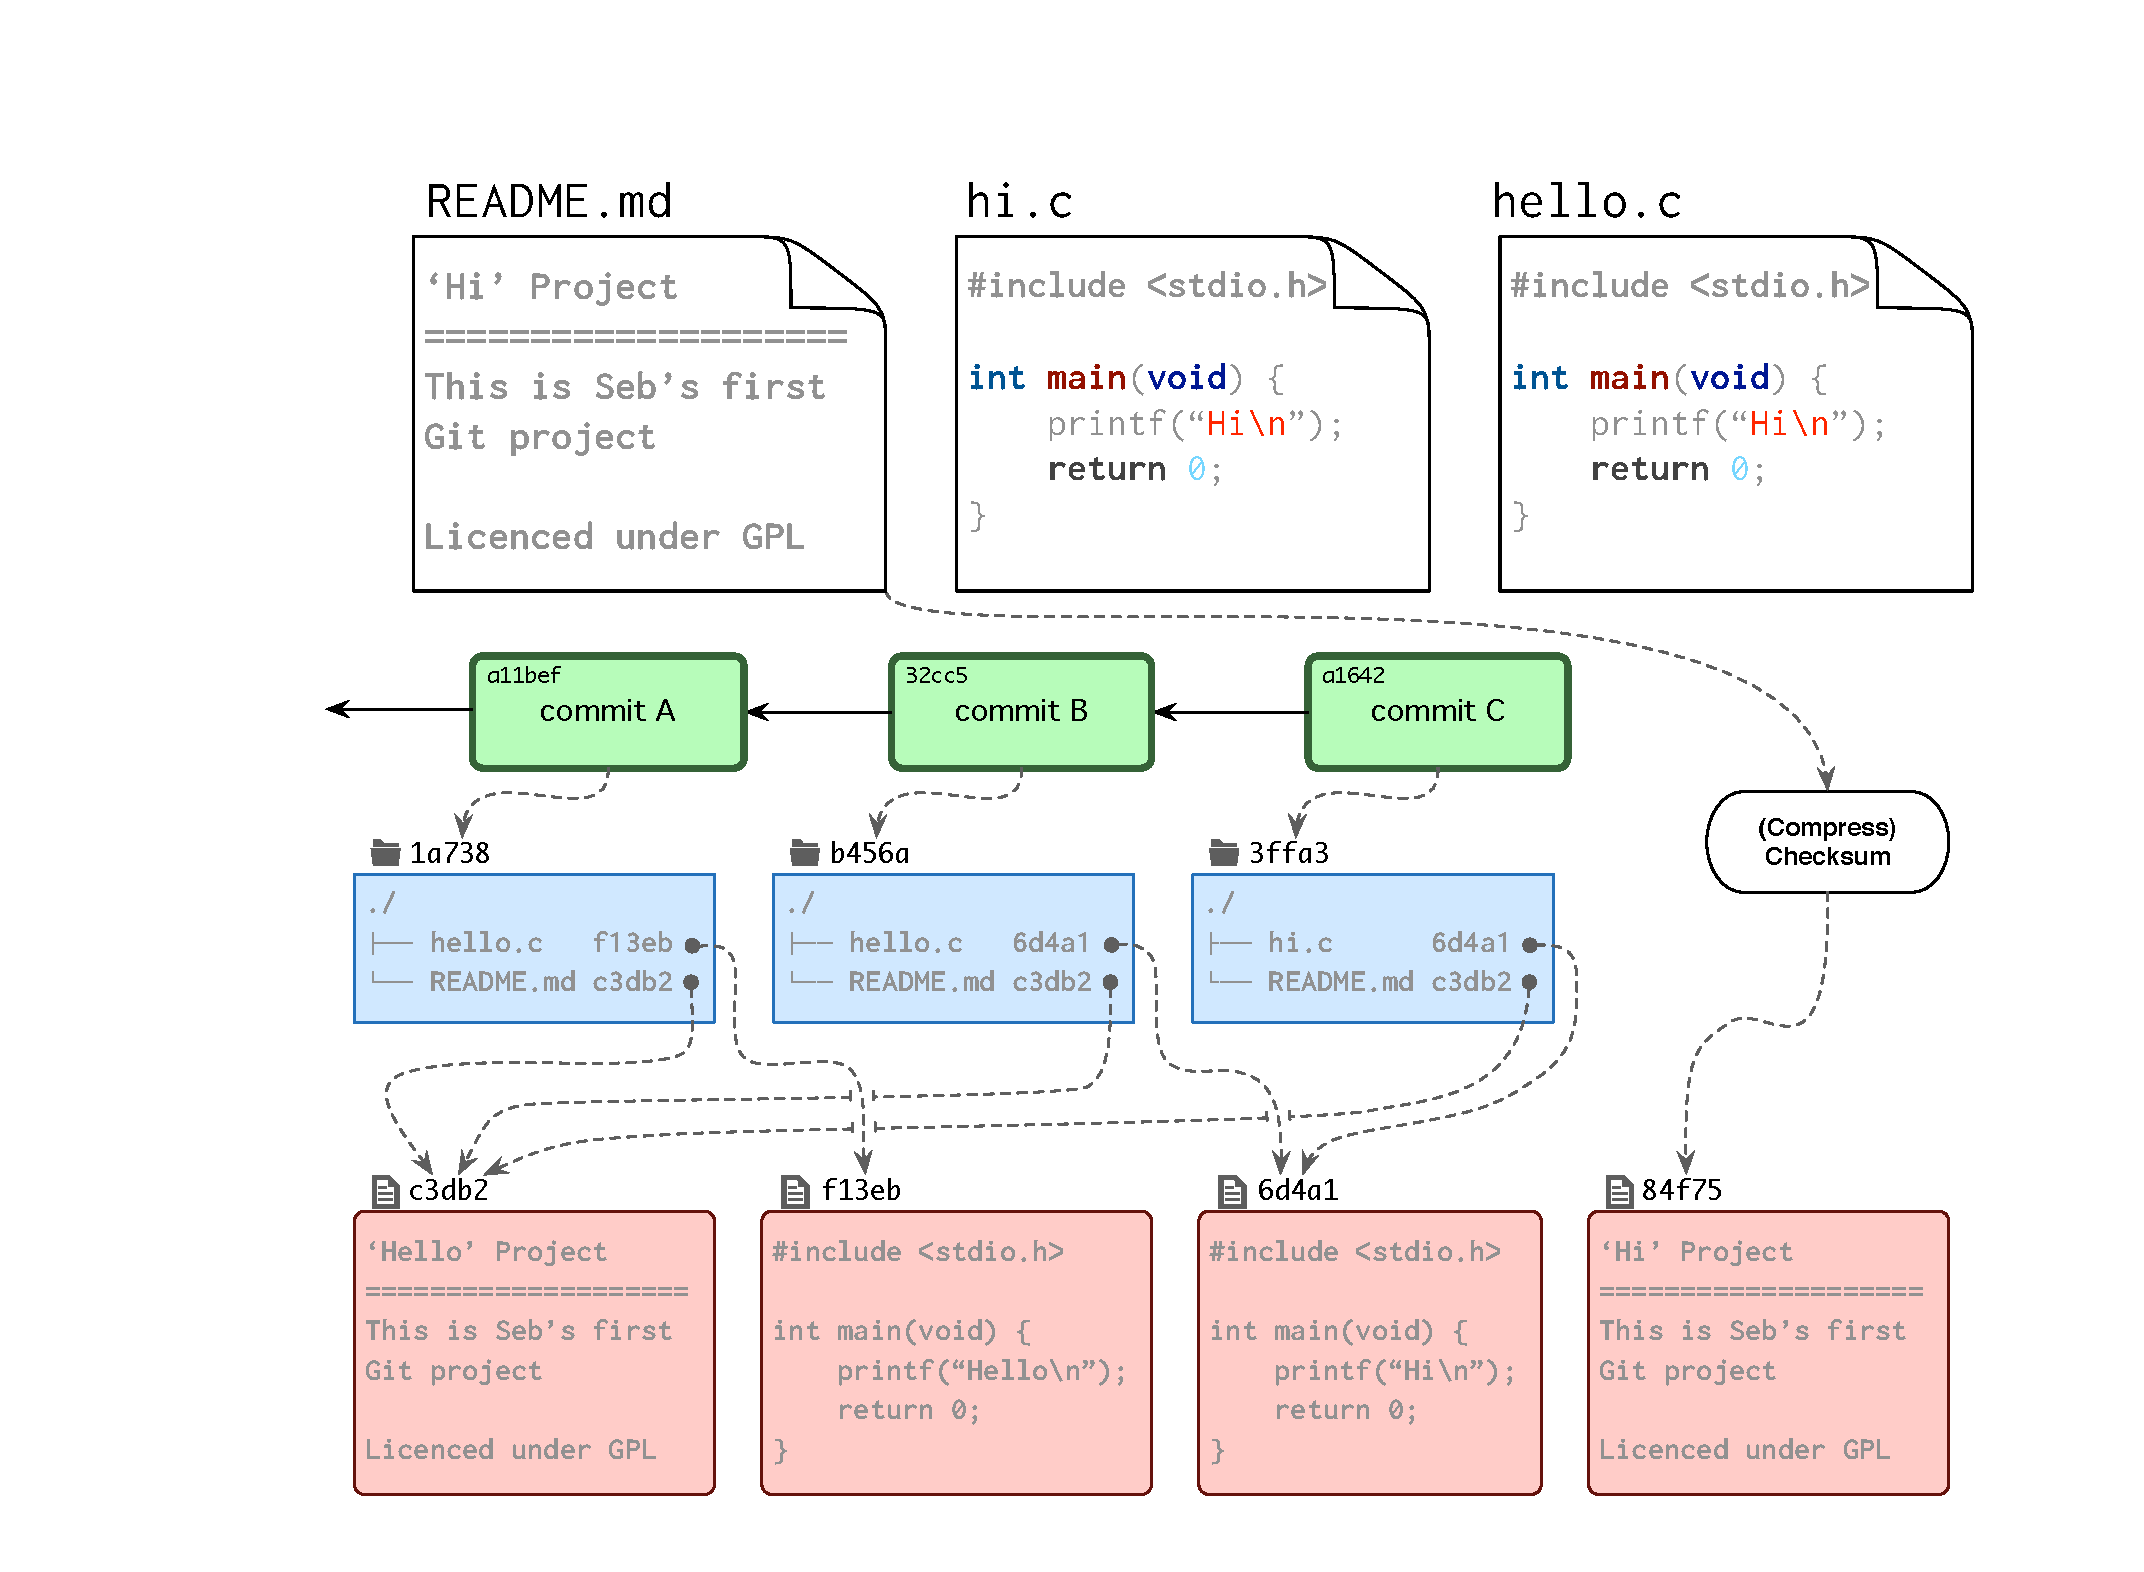
\includegraphics[height=0.95\textheight]{delta_vs_snapshot_example-131.pdf}}
  \only<32>{\includegraphics[height=0.95\textheight]{delta_vs_snapshot_example-132.pdf}}
  \only<33>{\includegraphics[height=0.95\textheight]{delta_vs_snapshot_example-133.pdf}}
  \only<34>{\includegraphics[height=0.95\textheight]{delta_vs_snapshot_example-134.pdf}}
  \only<35>{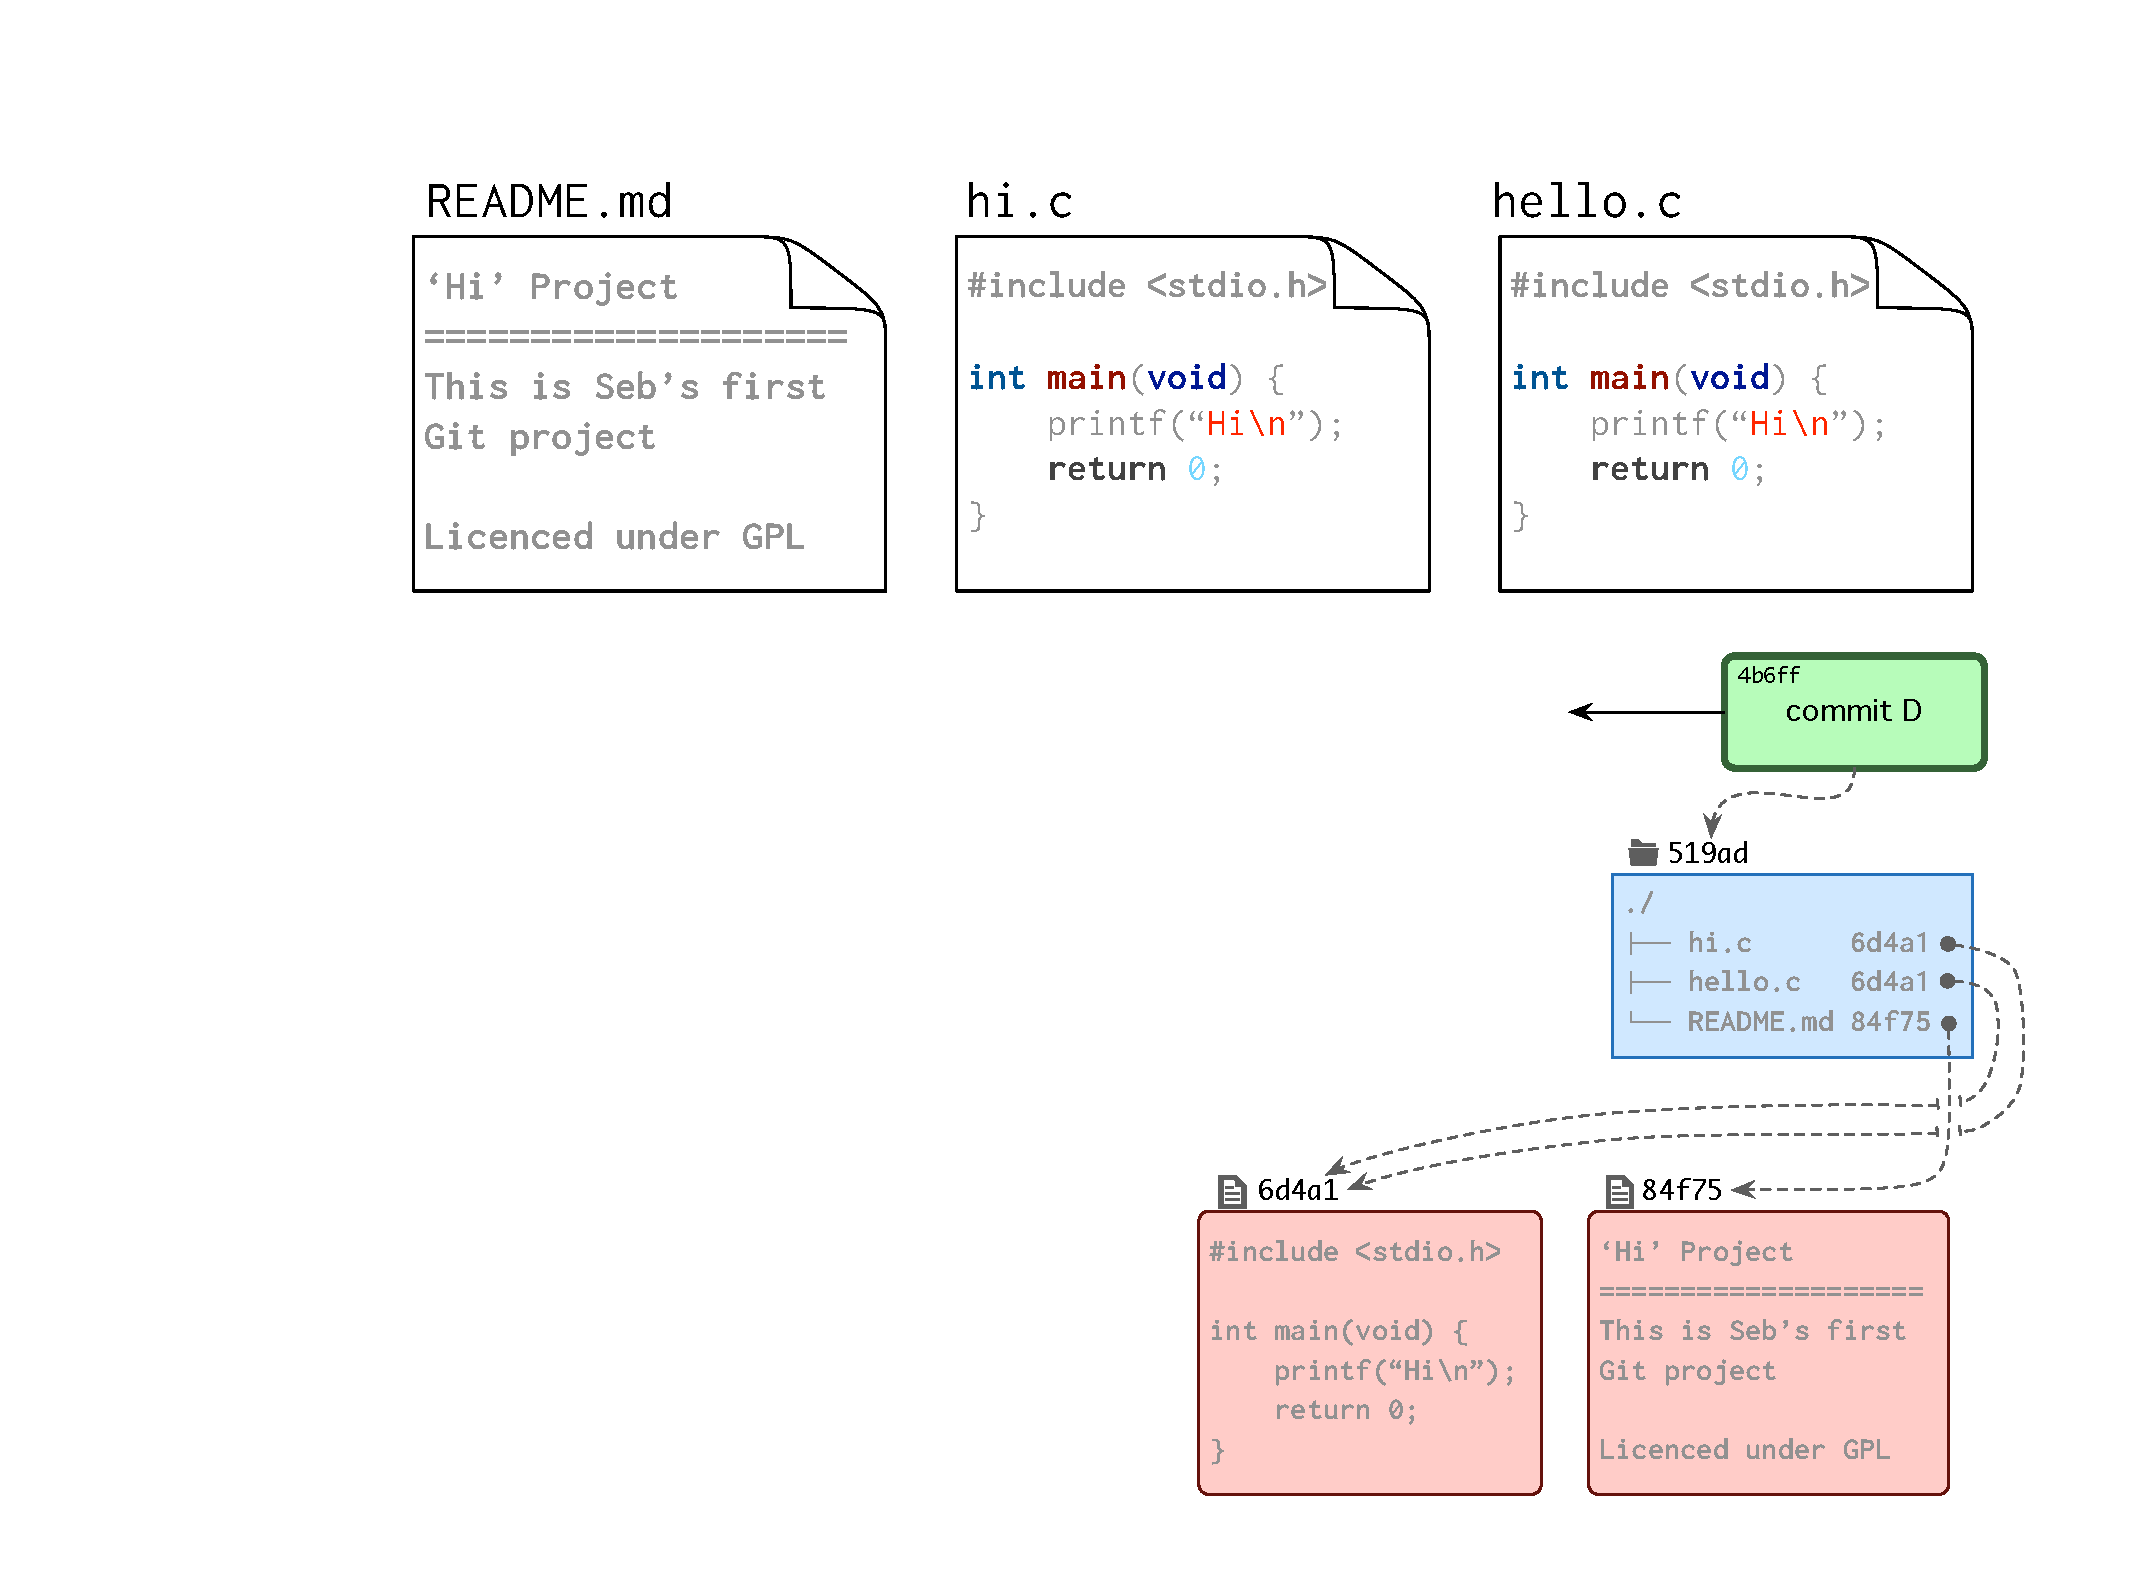
\includegraphics[height=0.95\textheight]{delta_vs_snapshot_example-135.pdf}}
  \only<36>{\includegraphics[height=0.95\textheight]{delta_vs_snapshot_example-136.pdf}}

}





% ~~~~~~~~~~~~~~~~~~~~~~~~~~~~~~~~~~~~~~~~~~~~~~~~~~~~~~~~~~~~~~~~
% eof
% 
% Local Variables:
% mode: latex
% mode: flyspell
% mode: visual-line
% TeX-master: "intro_git"
% End:



\setcounter{framenumber}{\value{finalframe}}

\end{document}

% ~~~~~~~~~~~~~~~~~~~~~~~~~~~~~~~~~~~~~~~~~~~~~~~~~~~~~~~~~~~~~~~~
% eof
% 
% Local Variables:
% mode: latex
% mode: flyspell
% mode: visual-line
% TeX-master: "git.tex"
% End:
